\documentclass[10pt,a4paper]{amsart}
\usepackage{amsmath,amssymb,amsthm,graphicx}
\usepackage{hyperref}
\numberwithin{equation}{section}

%\usepackage{amsfonts}
%\usepackage{amsmath, %full page, tikz-cd, %comment, %amsthm%amssymb, amscd, graphicx, %showkeys}
\usepackage{tikz-cd,enumitem}
%\usepackage{xcolor}


\newtheorem{thm}{Theorem}[section]
\newtheorem{defn}[thm]{Definition}
\newtheorem{prop}[thm]{Proposition}
\newtheorem{cor}[thm]{Corollary}
\newtheorem{lem}[thm]{Lemma}
\newtheorem{conj}[thm]{Conjecture}

\theoremstyle{definition}
\newtheorem{rema}[thm]{Remark}
\newtheorem{app}[thm]{Application}
\newtheorem{prob}[thm]{Problem}
\newtheorem{conv}[thm]{Convention}
\newtheorem{cond}[thm]{Condition}
\newtheorem{assum}[thm]{Assumption}
\newtheorem{exam}[thm]{Example}

\newcommand{\nn}{\nonumber \\}

 \newcommand{\sgn}{\operatorname{sgn}}
 \newcommand{\res}{\operatorname{Res}}
 \newcommand{\ord}{\operatorname{ord}}
\newcommand{\hol}{\operatorname{Hol}}
\renewcommand{\hom}{\operatorname{Hom}}
\newcommand{\edo}{\operatorname{End}}
% \newcommand{\pf}{{\it Proof.}\hspace{2ex}}
 \newcommand{\epf}{\hspace*{\fill}\mbox{$\halmos$}}
 \newcommand{\epfv}{\hspace*{\fill}\mbox{$\halmos$}\vspace{1em}}
 \newcommand{\epfe}{\hspace{2em}\halmos}
\newcommand{\nord}{\mbox{\scriptsize ${\circ\atop\circ}$}}
\newcommand{\wt}{\mbox{\rm wt}\,}
\newcommand{\swt}{\mbox{\rm {\scriptsize wt}}\,}
\newcommand{\lwt}{\mbox{\rm wt}^{L} }
\newcommand{\rwt}{\mbox{\rm wt}^{R} }
\newcommand{\slwt}{\mbox{\rm {\scriptsize wt}}^{L}\,}
\newcommand{\srwt}{\mbox{\rm {\scriptsize wt}}^{R}\,}
\newcommand{\clr}{\mbox{\rm clr}\ }
\newcommand{\mbar}{\big\vert}
\newcommand{\lbar}{\big\vert}
\newcommand{\tr}{\operatorname{Tr}}
\newcommand{\A}{\mathcal{A}}
\newcommand{\Y}{\mathcal{Y}}
\newcommand{\C}{\mathbb{C}}
\newcommand{\Z}{\mathbb{Z}}
\newcommand{\R}{\mathbb{R}}
\newcommand{\Q}{\mathbb{Q}}
\newcommand{\N}{\mathbb{N}}
\newcommand{\CN}{\mathcal{N}}
\newcommand{\F}{\mathcal{F}}
\newcommand{\I}{\mathbb{I}}
\newcommand{\V}{\mathcal{V}}
\newcommand{\one}{\mathbf{1}}
\newcommand{\BY}{\mathbb{Y}}
\newcommand{\ds}{\displaystyle}
\renewcommand{\mod}{\operatorname{mod}}
\newcommand{\g}{\mathfrak{g}}
\newcommand{\tio}{\text{twisted intertwining operator}}
\renewcommand{\i}{\mathrm{i}}
\newcommand{\PB}{{\rm PB}}


 \makeatletter
\newlength{\@pxlwd} \newlength{\@rulewd} \newlength{\@pxlht}
\catcode`.=\active \catcode`B=\active \catcode`:=\active \catcode`|=\active
\def\sprite#1(#2,#3)[#4,#5]{
 \edef\@sprbox{\expandafter\@cdr\string#1\@nil @box}
 \expandafter\newsavebox\csname\@sprbox\endcsname
 \edef#1{\expandafter\usebox\csname\@sprbox\endcsname}
 \expandafter\setbox\csname\@sprbox\endcsname =\hbox\bgroup
 \vbox\bgroup
 \catcode`.=\active\catcode`B=\active\catcode`:=\active\catcode`|=\active
 \@pxlwd=#4 \divide\@pxlwd by #3 \@rulewd=\@pxlwd
 \@pxlht=#5 \divide\@pxlht by #2
 \def .{\hskip \@pxlwd \ignorespaces}
 \def B{\@ifnextchar B{\advance\@rulewd by \@pxlwd}{\vrule
 height \@pxlht width \@rulewd depth 0 pt \@rulewd=\@pxlwd}}
 \def :{\hbox\bgroup\vrule height \@pxlht width 0pt depth
0pt\ignorespaces}
 \def |{\vrule height \@pxlht width 0pt depth 0pt\egroup
 \prevdepth= -1000 pt}
 }
\def\endsprite{\egroup\egroup}
\catcode`.=12 \catcode`B=11 \catcode`:=12 \catcode`|=12\relax
\makeatother

\makeatletter
\newcommand{\raisemath}[1]{\mathpalette{\raisem@th{#1}}}
\newcommand{\raisem@th}[3]{\raisebox{#1}{$#2#3$}}
\makeatother


\makeatletter% subalign left alignment
\newcommand{\subalign}[1]{%
	\vcenter{%
		\Let@ \restore@math@cr \default@tag
		\baselineskip\fontdimen10 \scriptfont\tw@
		\advance\baselineskip\fontdimen12 \scriptfont\tw@
		\lineskip\thr@@\fontdimen8 \scriptfont\thr@@
		\lineskiplimit\lineskip
		\ialign{\hfil$\m@th\scriptstyle##$&$\m@th\scriptstyle{}##$\hfil\crcr
			#1\crcr
		}%
	}%
}
\makeatother


\def\hboxtr{\FormOfHboxtr} % Only necessary if
%\kern... is wanted
\sprite{\FormOfHboxtr}(25,25)[0.5 em, 1.2 ex] % Resolution ca. 200x340 dpi.


:BBBBBBBBBBBBBBBBBBBBBBBBB |
:BB......................B |
:B.B.....................B |
:B..B....................B |
:B...B...................B |
:B....B..................B |
:B.....B.................B |
:B......B................B |
:B.......B...............B |
:B........B..............B |
:B.........B.............B |
:B..........B............B |
:B...........B...........B |
:B............B..........B |
:B.............B.........B |
:B..............B........B |
:B...............B.......B |
:B................B......B |
:B.................B.....B |
:B..................B....B |
:B...................B...B |
:B....................B..B |
:B.....................B.B |
:B......................BB |
:BBBBBBBBBBBBBBBBBBBBBBBBB |





\endsprite

\def\shboxtr{\FormOfShboxtr} % Only necessary if
%\kern... is wanted
\sprite{\FormOfShboxtr}(25,25)[0.3 em, 0.72 ex] % Resolution ca. 200x340 dpi.


:BBBBBBBBBBBBBBBBBBBBBBBBB |
:BB......................B |
:B.B.....................B |
:B..B....................B |
:B...B...................B |
:B....B..................B |
:B.....B.................B |
:B......B................B |
:B.......B...............B |
:B........B..............B |
:B.........B.............B |
:B..........B............B |
:B...........B...........B |
:B............B..........B |
:B.............B.........B |
:B..............B........B |
:B...............B.......B |
:B................B......B |
:B.................B.....B |
:B..................B....B |
:B...................B...B |
:B....................B..B |
:B.....................B.B |
:B......................BB |
:BBBBBBBBBBBBBBBBBBBBBBBBB |

\endsprite

\usepackage{cleveref}
\crefname{originalreference}{original reference}{original references}
\Crefname{originalreference}{Original reference}{Original references}
\makeatletter
\newlabel{sec4}{{4}{source}{}{sourcepointer-1}{}}
\newlabel{sec4@cref}{{[originalreference][0][]4}{[1][0][]source}{}{}{}}
\makeatother
\crefname{originalreference}{original reference}{original references}
\Crefname{originalreference}{Original reference}{Original references}
\makeatletter
\newlabel{sec5}{{5}{source}{}{sourcepointer-2}{}}
\newlabel{sec5@cref}{{[originalreference][0][]5}{[1][0][]source}{}{}{}}
\makeatother
\title{Skew-symmetry and contragredient transformations of general twisted intertwining operators}
\author{Jishen Du, Yi-Zhi Huang}
\date{doi:10.3842/SIGMA.2026.086; CC BY 4.0}
\begin{document}
\maketitle
\noindent\textit{Allowed standard prerequisites (editorial).}\begin{itemize}
\item Vertex operator algebras, twisted modules and ordinary complex analytic continuation. Complete original bibliography and source-local definitions retained.
\end{itemize}\medskip
\ifdefined\hypertarget\hypertarget{sourcepointer-1}{}\fi
\noindent\textit{Source reference.} Original reference 4: algebra-geometry/sources/sigma-2026-086/native/sigma26-086.tex, source lines 2738--2738. Pointer to another section or introductory illustration; complete target construction and source-local proof support are retained.\par\medskip
\ifdefined\hypertarget\hypertarget{sourcepointer-2}{}\fi
\noindent\textit{Source reference.} Original reference 5: algebra-geometry/sources/sigma-2026-086/native/sigma26-086.tex, source lines 3539--3539. Pointer to another section or introductory illustration; complete target construction and source-local proof support are retained.\par\medskip
\section{Twisted modules and twisted intertwining operators}\label{sec2}

We first recall in this section the notion of (generalized) twisted module
from~\cite{H-log-twisted-mod}. We then introduce a~notion
of twisted intertwining
operators more general than the one in
\cite{H-twisted-int}. We also give some basic results on such
twisted intertwining operators.

For $z\in \C^{\times}$ and $p\in \Z$, we shall use the notation
$l_{p}(z)=\log |z|+{\rm i}\arg z+2\pi p {\rm i}$, where $0\le \arg z<2\pi$.
We shall also use the notation $\log z=l_{0}(z)=\log |z|+{\rm i}\arg z$.
For a~vector space~$U$,~${p\in \Z}$ and a~formal series
\[f(x)=\sum_{k=0}^{K}\sum_{n\in \C}a_{n, k}x^{n}(\log x)^{k},\]
where $a_{n, k}\in U$,
the series
\[f^{p}(z)=\sum_{k=0}^{K}\sum_{n\in \C}
a_{n, k}{\rm e}^{nl_{p}(z)}(l_{p}(z))^{k}\]
is called the $p$-th analytic branch of $f(x)$. We also denote
$f^{0}(z)$ simply by $f(z)$.

Let $V$ be a~vertex operator algebra and $g$ an automorphism of $V$.
We recall the definition of generalized $g$-twisted
$V$-module first introduced in~\cite{H-log-twisted-mod}.
Note that as in~\cite{H-log-twisted-mod,H-twisted-int} in this paper, the vertex operator map for a~generalized $g$-twisted $V$-module
in general contains the logarithm of the variable and the operator
$L(0)$ in general does not have to act semisimply.

\begin{defn}\label{twisted-mod}
A~{\it generalized $g$-twisted
$V$-module without a~$g$-action} is a~$\C$-graded
vector space~${W = \coprod_{n \in \C} W_{[n]}}$ {\rm(}graded by {\it weights}$)$
equipped with a~linear map
\begin{gather*}
Y_{W}^g\colon \ V\otimes W \to W\{x\}[\log x],\\
v \otimes w \mapsto Y_{W}^g(v, x)w=\sum_{k=0}^{K}\sum_{n\in \C}(Y_{W}^g)_{n, k}(v)wx^{-n-1}(\log x)^{k}
\end{gather*}
satisfying the following conditions:
\begin{enumerate}[label=$(\arabic*)$]\itemsep=0pt
\item The {\it equivariance property}: For $p \in \mathbb{Z}$, $z
\in \mathbb{C}^{\times}$, $v \in V$ and $w \in W$,
$\bigl(Y^{g}_{W}\bigr)^{p + 1}(gv,
z)w = \bigl(Y^{g}_{W}\bigr)^{p}(v, z)w$,
where for $p \in \mathbb{Z}$, $\bigl(Y^{g}_{W}\bigr)^{ p}(v, z)$
is the $p$-th analytic branch of $Y_{W}^g(v, x)$.

\item The {\it identity property}: For $w \in W$, $Y^g_{W}({\bf 1}, x)w
= w$.

\item The {\it duality property}: For
any $u, v \in V$, $w \in W$ and $w' \in W'$, there exists a~maximally-extended
multivalued analytic function with preferred branch of the form
\[
f(z_1, z_2) = \sum_{i,
j, k, l = 0}^N a_{ijkl}z_1^{m_i}z_2^{n_j}(\operatorname{log}z_1)^k({\rm
log}z_2)^l(z_1 - z_2)^{-t}
\]
for $N \in \mathbb{N}$, $m_1, \dots,
m_N$, $n_1, \dots, n_N \in \mathbb{C}$ and $t \in \mathbb{Z}_{+}$,
such that the series
\begin{gather*}
\big\langle w', \bigl(Y^{g}_{W}\bigr)^{ p}(u, z_1)\bigl(Y^{g}_{W}\bigr)^{p}(v,
z_2)w\big\rangle = \sum_{n \in \mathbb{C}}\big\langle w', \bigl(Y^{g}_{W}\bigr)^{ p}(u,
z_1)\pi_n\bigl(Y^{g}_{W}\bigr)^{ p}(v, z_2)w\big\rangle,
\\
\big\langle w', \bigl(Y^{g}_{W}\bigr)^{ p}(v,
z_2)\bigl(Y^{g}_{W}\bigr)^{p}(u, z_1)w\big\rangle = \sum_{n \in \mathbb{C}}\big\langle w',
\bigl(Y^{g}_{W}\bigr)^{ p}(v, z_2)\pi_n\bigl(Y^{g}_{W}\bigr)^{ p}(u, z_1)w\big\rangle,
\\
\big\langle w', \bigl(Y^{g}_{W}\bigr)^{ p}(Y_{V}(u, z_1 - z_2)v,
z_2)w\big\rangle = \sum_{n \in \mathbb{C}}\big\langle w', \bigl(Y^{g}_{W}\bigr)^{
p}(\pi_nY_{V}(u, z_1 - z_2)v, z_2)w\big\rangle
\end{gather*}
are absolutely convergent on
the regions $|z_1| > |z_2| > 0$, $|z_2| > |z_1| > 0$, $|z_2| > |z_1
- z_2| > 0$, respectively, and their sums are equal to the branch
\[
f^{p,p}(z_{1}, z_{2})= \sum_{i, j, k, l = 0}^N
a_{ijkl}{\rm e}^{m_il_p(z_1)}{\rm e}^{n_jl_p(z_2)}l_p(z_1)^kl_p(z_2)^l(z_1 -
z_2)^{-t}
\]
of $f(z_1, z_2)$ on the region $|z_1| > |z_2| > 0$, the region $|z_2| > |z_1| > 0$,
the region given by $|z_2| > |z_1- z_2| > 0$ and $|{\arg z_{1}-\arg z_{2}}|<\frac{\pi}{2}$, respectively.


\item The {\it $L(0)$-grading condition}:
Let $L_{W}^{g}(0)=\res_{x}xY_{W}^g(\omega, x)$. Then for $n\in \C$,
$w \in W_{[n]}$,
there exists $K\in \Z_{+}$ such that \smash{$\bigl(L_{W}^g (0)-n\bigr)^{K} w
=0$}.

\item The $L(-1)$-{\it derivative property}: For $v \in V$,
\[
\frac{\rm d}{{\rm d}x}Y^g_{W}(v, x) = Y^g_{W}(L_{V}(-1)v, x).
\]

\end{enumerate} A~{\it lower-bounded generalized $g$-twisted $V$-module}
is a~generalized $g$-twisted
$V$-module $W$ such that
for each ${n\in \C}$, $W_{[n + l]} = 0$ for
sufficiently negative real numbers $l$. A~generalized $g$-twisted $V$-module $W$
is said to be {\it grading-restricted} if it is lower
bounded and for each ${n \in \mathbb{C}}$, \smash{$\dim W_{[n]}<\infty$}. A~{\it generalized $g$-twisted $V$-module with a~$g$-action} is a~${\C}\times \C/\Z$-graded
vector space \smash{$W = \coprod_{n \in \C, \alpha\in \C/\Z} W_{[n]}^{[\alpha]}$} {\rm(}graded by {\it weights} and {\it $g$-weights}{\rm)}
equipped with a~linear map \smash{$Y_{W}^g\colon V\otimes W \to W\{x\}[\log x]$} as above and an action of $g$
such that $W$ equipped with $Y_{W}^g$ is a~generalized $g$-twisted $V$-module
without a~$g$-action satisfying in addition the following {\it $g$-grading condition}:
There exists $\Lambda\in \Z_{+}$ such that for $\alpha\in \C/\Z$,
\smash{$w \in W^{[\alpha]}=\coprod_{n\in \N}W_{[n]}^{[\alpha]}$}, \smash{$\bigl(g-{\rm e}^{2\pi \alpha{\rm i}}\bigr)^{\Lambda}w=0$}. Moreover,
$gY_{W}^{g}(u,x)w=Y_{W}^{g}(gu,x)gw$ for $u\in V$ and $w\in W$.
\end{defn}

Module maps between $g$-twisted $V$-modules are defined in the obvious way.
For two different automorphisms $g_{1}$ and $g_{2}$ of $V$, there might exist
linear maps from a~$g_{1}$-twisted $V$-module to a~$g_{2}$-twisted $V$-module commuting with the twisted vertex operator maps when
$V$ is not simple. But we will not consider such maps in this paper. So in the
categories of twisted $V$-modules considered in this paper,
we always choose the space of
 module maps between a~$g_{1}$-twisted $V$-module and a~$g_{2}$-twisted $V$-module
to be $0$ if $g_{1}\ne g_{2}$.

In this paper, generalized $g$-twisted $V$-modules with or without $g$-actions
are all called {\it generalized $g$-twisted $V$-modules}. Only when the $g$-actions are specifically discussed,
we shall add the words ``with a~$g$-action'' or ``without a~$g$-action''. Later, we shall also need
generalized $g$-twisted $V$-modules with $g$-actions equipped with an $h$-action for another
automorphism $h$ of $V$.
Also, for simplicity, we shall sometimes omit the subscript
$W$ to denote the twisted vertex operator map~$Y_{W}^{g}$
by $Y^{g}$.

\begin{rema}
Note that a~lower-bounded generalized
$g$-twisted $V$-module defined above also satisfies
the lower-truncation property: For $v\in V$ and $w\in W$, $n\in \C$ and $k=0, \dots, K$,
\smash{$\bigl(Y_{W}^g\bigr)_{n+l, k}(w_{1})w_{2}=0$} for $l\in \N$ sufficiently large.
This in fact follows from the $L(0)$-commutator formula,
which is a~consequence of the duality property and the $L(0)$-grading condition.
\end{rema}

\begin{rema}
In this paper, we need to study generalized $g$-twisted $V$-modules with and without
$g$-actions in a~different way because the skew-symmetry and contragredient isomorphisms in Section \ref{sec3} are different in these two types
of twisted modules. In fact, there is also a~notion of generalized $g$-twisted module with a~$G$ action for a~group $G$ of automorphisms of $V$. See~\cite{H-cofinite-P(z)} for a~definition and
the construction $P(z)$-tensor product of such twisted modules.
\end{rema}

In this paper, we shall consider only lower-bounded generalized $g$-twisted $V$-modules and grading-restricted
generalized $V$-modules. For simplicity, we shall often call lower-bounded generalized
$g$-twisted $V$-modules simply $g$-twisted $V$-modules and
grading-restricted
generalized $V$-modules simply grading-restricted $g$-twisted $V$-modules.

Let $\bigl(W, Y^{g}_{W}\bigr)$ be a~$g$-twisted
$V$-module without a~$g$-action. Let $h$ be an automorphism of~$V$. We recall
the $hgh^{-1}$-twisted
$V$-module $\bigl(W, \phi_{h}\bigl(Y^{g}_{W}\bigr)\bigr)$ without a~$hgh^{-1}$-action (see, for example,~\cite{H-twisted-int}).
Let
\begin{gather*}
\phi_{h}\bigl(Y^{g}_{W}\bigr)\colon\ V\times W\to W\{x\}[\operatorname{log} x],\qquad
v \otimes w \mapsto \phi_{h}\bigl(Y^{g}_{W}\bigr)(v, x)w
\end{gather*}
be the linear map defined by{\samepage
\[\phi_{h}\bigl(Y^{g}_{W}\bigr)(v, x)w=Y^{g}_{W}\bigl(h^{-1}v, x\bigr)w.\]
Then the pair $\bigl(W, \phi_{h}\bigl(Y^{g}_{W}\bigr)\bigr)$ is an $hgh^{-1}$-twisted
$V$-module without a~$hgh^{-1}$-action.}

In the case that $W$ is a~$g$-twisted $V$-module
with a~$g$-action and also has an action
of $h$ in the sense that $W$ is a~module for the group generated by $g$ and $h$, we define
\begin{gather*}
\varphi_{h}\bigl(Y^{g}_{W}\bigr)\colon\ V\times W\to W\{x\}[\operatorname{log} x],\qquad
v \otimes w \mapsto \varphi_{h}\bigl(Y^{g}_{W}\bigr)(v, x)w
\end{gather*}
by
\[\varphi_{h}\bigl(Y^{g}_{W}\bigr)(v, x)w=hY^{g}_{W}\bigl(h^{-1}v, x\bigr)h^{-1}w.\]
Then $\bigl(W, \varphi_{h}\bigl(Y^{g}_{W}\bigr)\bigr)$ is also an $hgh^{-1}$-twisted
$V$-module without a~$hgh^{-1}$-action.
Since the conformal element $\omega$ is fixed under the action of
$g^{-1}$, the coefficients
\[L_{\varphi_{h}(W)}(n)=\res_{x}x^{n+1}\varphi_{h}\bigl(Y^{g}_{W}\bigr)(\omega, x)
=h\res_{x}x^{n+1}Y_{W}^{g}(\omega, x)h^{-1}=hL_{W}^{g}(n)h^{-1}\]
 of the vertex operator $\varphi_{h}\bigl(Y^{g}_{W}\bigr)(\omega, x)$ for $n\in \N$
also give Virasoro operators on $W$ with the same central charge.
Since $h$ is an isomorphism of the vector space $W$,
\[hW=\coprod_{n\in \C, \alpha\in \C/\Z}hW_{[n]}^{[\alpha]}.\]
We denote the graded space $hW$ by $\varphi_{h}(W)$ and
\smash{$hW_{[n]}^{[\alpha]}$} by \smash{$\varphi_{h}(W)_{[n]}^{[\alpha]}$}
$n\in \C, \alpha\in \C/\Z$. Then we have
\[\varphi_{h}(W)=\coprod_{n\in \C, \alpha\in \C/\Z}\varphi_{h}(W)_{[n]}^{[\alpha]}.\]
Note that as a~vector space $\varphi_{h}(W)=hW$ is the same as $W$, but as graded spaces,
they are different.
For \smash{$w\in \varphi_{h}(W)_{[n]}=\coprod_{\alpha\in \C/\Z}\varphi_{h}(W)_{[n]}^{[\alpha]}$},
\smash{$h^{-1}w\in W_{[n]}=\coprod_{\alpha\in \C/\Z}W_{[n]}^{[\alpha]}$}. So there exists ${K\in \Z_{+}}$ such that \smash{$\bigl(L_{W}^{g}-n\bigr)^{K}h^{-1}w=0$}. Then
\[
(L_{\varphi_{h}(W)}(0)-n)^{K}w=h\bigl(L_{W}^{g}-n\bigr)^{K}h^{-1}w=0.
\]
For \smash{$w\in \varphi_{h}(W)^{[\alpha]}=\coprod_{n\in \Z}\varphi_{h}(W)_{[n]}^{[\alpha]}$},
\smash{$h^{-1}w\in W^{[\alpha]}=\coprod_{n\in \Z}W_{[n]}^{[\alpha]}$}. So there exists
$\Lambda\in \Z_{+}$ such that \smash{$\bigl(g-{\rm e}^{2\pi {\rm i}\alpha}\bigr)^{\Lambda}h^{-1}w=0$}.
Then \smash{$\bigl(hgh^{-1}-{\rm e}^{2\pi {\rm i}\alpha}\bigr)^{\Lambda}w=h\bigl(g-{\rm e}^{2\pi {\rm i}\alpha}\bigr)^{\Lambda}h^{-1}w=0$}.
Also we have
\begin{align*}
hgh^{-1}\varphi_{h}\bigl(Y^{g}_{W}\bigr)(v, x)w&=hgY^{g}_{W}\bigl(h^{-1}v, x\bigr)h^{-1}w=hY^{g}_{W}\bigl(h^{-1}hgh^{-1}v, x\bigr)h^{-1}hgh^{-1}w\\
&=\varphi_{h}\bigl(Y^{g}_{W}\bigr)\bigl(hgh^{-1}v, x\bigr)hgh^{-1}w.
\end{align*}
So $(\varphi_{h}(W), \varphi_{h}\bigl(Y^{g}_{W}\bigr))$ is a~$hgh^{-1}$-twisted $V$-module with an
$hgh^{-1}$-action.
We shall denote this $hgh^{-1}$-twisted
$V$-module with an
$hgh^{-1}$-action by $\varphi_{h}(W)$.

Note that when $h=g$, $\varphi_{h}(W)=W$ and
$\phi_{g}(W)$ with the twisted vertex operator
given by
\[\phi_{g}\bigl(Y^{g}_{W}\bigr)(v, x)w=Y^{g}_{W}\bigl(g^{-1}v, x\bigr)w\]
is equivalent to the original
$g$-twisted module $W$ with the equivalence $g^{-1}\colon W\to W$. By the equivariance property,
we have \smash{$\bigl(Y^{g}_{W}\bigr)^{p}\bigl(g^{-1}v, x\bigr)=\bigl(Y^{g}_{W}\bigr)^{p+1}(v, x)$}
and, if
\[Y^{g}_{W}(v, x)w=\sum_{k=0}^{K}\sum_{n\in \C}
\bigl(Y^{g}_{W}\bigr)_{n, k}(v)x^{-n-1}(\log x)^{k}\]
for $v\in V$ and $w\in W$,
we have
\[Y^{g}_{W}\bigl(g^{-1}v, x\bigr)w=\sum_{k=0}^{K}\sum_{n\in \C}
\bigl(Y^{g}_{W}\bigr)_{n, k}(v){\rm e}^{-2\pi {\rm i} n}x^{-n-1}(\log x+2\pi {\rm i})^{k}.\]

\begin{rema}
 In the definitions of $\bigl(\varphi_{h}(W), \varphi_{h}\bigl(Y_{W}^{g}\bigr)\bigr)$,
we assume that there is an action of~$h$ on~$W$. One immediate question is whether
there exist such $g$-twisted $V$-modules with $h$-actions. In fact, the same construction
in Section \ref{sec5} of~\cite{H-const-twisted-mod} can be used to construct such a~$g$-twisted $V$-module with an $h$-action
or even a~$g$-twisted $V$-module with a~$G$-action for a~group~$G$ of automorphisms of $V$ satisfying
the additional condition $hY_{W}^{g}(v, x)w=Y_{W}^{g}(hv, x)hw$ for~${h\in G}$. In this case, though
$\varphi_{h}(W)=W$ as vector spaces and
$\varphi_{h}\bigl(Y_{W}^{g}\bigr)=Y_{W}^{g}$ as linear maps from~${V\otimes W}$ to $W\{x\}[\log x]$ when we view
$\varphi_{h}(W)$ as a~vector space equal to $W$, $\varphi_{h}(W)$ is graded by generalized eigenspaces of $hgh^{-1}$
but $W$is graded by the generalized eigenspaces of $g$.
In particular, $\bigl(\varphi_{h}(W), \varphi_{h}\bigl(Y_{W}^{g}\bigr)\bigr)$ and $\bigl(W, Y_{W}^{g}\bigr)$ are indeed different twisted $V$-modules.
\end{rema}

We also recall contragredient twisted $V$-modules (see, for example, \cite{H-twisted-int}).
Let $\bigl(W, Y^{g}_{W}\bigr)$ be a~$g$-twisted $V$-module relative to $G$.
Let $W'$ be the graded dual of $W$. Define a~linear map
\begin{gather*}
\bigl(Y_{W}^{g}\bigr)'\colon\ V\otimes W' \to W'\{x\}[\operatorname{log} x],\qquad
v \otimes w' \mapsto \bigl(Y^g_{W}\bigr)'(v, x)w'
\end{gather*}
by
\[\big\langle \bigl(Y^g_{W}\bigr)'(v, x)w', w\big\rangle=\big\langle w', Y^{g}_{W}\bigl({\rm e}^{xL(1)}\bigl(-x^{-2}\bigr)^{L(0)}v, x^{-1}\bigr)w\big\rangle\]
for $v\in V$, $w\in W$ and $w'\in W'$.
Then the pair $\bigl(W', \bigl(Y^{g}_{W}\bigr)'\bigr)$ is a~$g^{-1}$-twisted $V$-module.


Let $M^{2}=\big\{(z_{1}, z_{2})\in \C^{2}\mid z_{1}\ne 0,\, z_{2}\ne 0,\,
z_{1}\ne z_{2}\big\}$.
Let $f(z_{1}, z_{2})$ be a~maximally extended
multivalued analytic function
on $M^{2}$
with a~preferred single-valued branch $f^{e}(z_{1}, z_{2})$
on the simply-connected
region $M^{2}_{0}$ given by
cutting $M^{2}$ along the positive real lines in the $z_{1}$-, $z_{2}$- and
$(z_{1}-z_{2})$-planes, that is, the sets
\begin{gather*}
\big\{(z_{1}, z_{2})\in M^{2}\mid z_{1}\in \R_{+}\big\},\qquad
\big\{(z_{1}, z_{2})\in M^{2}\mid z_{2}\in \R_{+}\big\},\\
\big\{(z_{1}, z_{2})\in M^{2}\mid z_{1}-z_{2}\in \R_{+}\big\},
\end{gather*}
with these sets attached to the upper half $z_{1}$-, $z_{2}$- and
$(z_{1}-z_{2})$-planes, that is, the points in these sets are
viewed as limits in $M_{0}^{2}$ of sequences of points approaching them
from the upper $z_{1}$-, $z_{2}$- and
$(z_{1}-z_{2})$-planes. Note that given any point
$\bigl(z^{0}_{1}, z^{0}_{2}\bigr)\in M^{2}$
and any loop $\gamma$ in $M^{2}$ based at $\bigl(z^{0}_{1}, z^{0}_{2}\bigr)$, we obtain from
the preferred branch of $f(z_{1}, z_{2})$ another single-valued branch
by going around $\gamma$. The resulting single-valued branch
depends only on the homotopy class of the loop and is independent of
the choices of the base point. Thus we obtain a~right action of the
fundamental group of $M^{2}$ on the set of single-valued
branches of $f(z_{1}, z_{2})$. Note that $M^{2}$ is
homotopically equivalent to the configuration space
\[F_{3}(\C)=\big\{(z_{1}, z_{2}, z_{3})\in \C^{3}\mid
z_{i}\ne z_{j},\, i\ne j\big\}.\]
So the fundamental group of $M^{2}$
is in fact the pure braid group $\PB_{3}$ and has three generators~$b_{12}$,~$b_{13}$ and $b_{23}$, which are given as follows:
Choose the base point
to be $(-3, -2)$. Then the generator $b_{12}$
is the homotopy class of the loop given by letting $z_{1}$ go
counterclockwise around the circle of radius $1$
centered at $-2$ (see Figure~\ref{b12}).
\begin{figure}[!b]
\centering
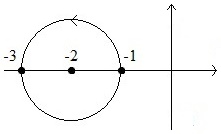
\includegraphics[scale=0.6]{b12}
\caption{The loop for $b_{12}$.}\label{b12}
\end{figure}
The generator $b_{23}$ is the homotopy class of
the loop given by letting $z_{2}$ go counterclockwise
around the circle of radius $2$ centered at $0$ (see Figure~\ref{b23}).
\begin{figure}[!t]
\centering
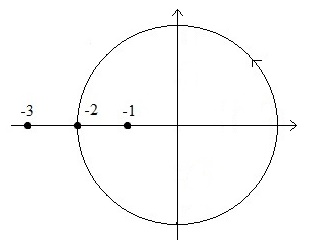
\includegraphics[scale=0.6]{b23}
\caption{The loop for $b_{23}$.}\label{b23}
\end{figure}
The generator $b_{13}$
is the homotopy class of the loop given by letting
$z_{1}$ go around first the lower half circle
of radius $3$ centered at $0$ counterclockwise, then the upper half circle
of radius $2$ centered at $1$ counterclockwise and finally the
lower half circle of radius $1$ centered at $-2$ clockwise (see Figure~\ref{b13}).
\begin{figure}[!t]
\centering
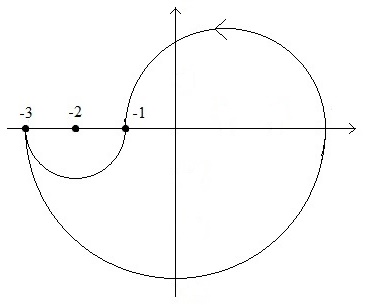
\includegraphics[scale=0.6]{b13}
\caption{The loop for $b_{13}$.}\label{b13}
\end{figure}
We know that the pure braid group $\PB_3$ is isomorphic to the
group generated by $b_{12}$, $b_{13}$, $b_{23}$ with the relations
$
b_{13}b_{12}b_{23}=b_{12}b_{23}b_{13}=b_{23}b_{13}b_{12}$.
See
\cite{D} for more detailed discussions on $M^{2}$, its fundamental group,
the pure braid groups and
multivalued functions on $M^{2}$.

For $a\in \PB_{3}$,
we denote the single-valued branch of $f(z_{1}, z_{2})$
obtained by applying
$a$ to $f^{e}(z_{1}, z_{2})$
by $f^{a}(z_{1}, z_{2})$.

Let $\delta=(\delta_1,\dots,\delta_n)$, where $\delta_i\in\{0,\infty\}$,
	$i=1,\dots,n$. Suppose $f(z_1,\dots,z_n)$ is a~multi-valued analytic
	function defined on an open region $\Omega$ of $\C^n$. We say
	$(z_1,\dots,z_n)=\delta$ is a~{\it component-isolated singularity
	of $f(z_1,\dots,z_n)$} if there exists $r=(r_{1}, \dots, r_{n})\in \R_{+}^n$ such that
	$\Delta^\times(\delta,r)\subset\Omega$, where
$\Delta^\times(\delta,r)=\{(z_{1}, \dots, z_{n})\in \C^{n}\mid |z_{i}|>r_{i} \text{ if } \delta_{i}=\infty,
0< |z_{i}|<r_{i} \text{ if } \delta_{i}=0\}$.
	Let~${A\in\operatorname{GL}(n,\C)}$
	and $\beta\in\C^n$ (written as a~row vector).
Then $\zeta_{1}, \dots, \zeta_{n}$ given by
\[(\zeta_1,\dots,\zeta_n)=(z_{1}, \dots, z_{n})A-\beta\]
are also independent variables. Define
	\begin{equation}\label{isolated}
	g(\zeta_1,\dots,\zeta_n)=f\left((\zeta_1,\dots,\zeta_n)
	A^{-1}+\beta A^{-1}\right).
	\end{equation}
For $\delta\in (\C\cup \{\infty\})^{n}$, we say that
$(\zeta_{1}, \dots, \zeta_{n})=\delta$ is a~{\it component-isolated singularity
of the function $f(z_1,\dots,z_n)$}
	if $(\zeta_{1}, \dots, \zeta_{n})=\delta$ is a~component-isolated singularity of
	$g(\zeta_1,\dots,\zeta_n)$.
	
\begin{rema}
{\rm Notice that $(\zeta_1,\dots,\zeta_n)(=(z_{1}, \dots, z_{n})A-\beta)
=\delta$ being a~component-isolated singularity
of a~function is not equivalent to
$(z_1,\dots,z_n)=\delta A^{-1}+\beta A^{-1}$ being a~component-isolated singularity of the same function.
This is because we have different sets of independent variables. For example, consider
$f(z_1,z_2)=\frac{1}{z_1-z_2}$. Since $(\zeta_1,\zeta_2)=(0,0)$ is a~component-isolated
singularity of the function $g(\zeta_1,\zeta_2)=1/\zeta_1$, we also say that
$(z_1-z_2,z_2)=(0,0)$ is a~component-isolated singularity of $f(z_1,z_2)$.
In this case, $z_{1}-z_{2}$ and $z_{2}$ are independent variables.
However, $(z_1,z_2)=(0,0)$ is clearly not a~component-isolated singularity of $f(z_1,z_2)$.
In this case, the independent variables are $z_{1}$ and $z_{2}$. }
\end{rema}

\begin{defn}
{\rm Let $f(z_1,\dots,z_n)$ be a~multi-valued analytic function defined on
an open region of $\C^n$. Let $\delta=(\delta_{1},\dots,\delta_n)
\in \{0,\infty\}^n$. Suppose $(z_1,\dots,z_n)=\delta$ is a~component-isolated
 singularity of $f(z_1,\dots,z_n)$. Let $\{f^b(z_1,\dots,z_n)\}_{b\in B}$
 be the set of all single valued branches of $f(z_1,\dots,z_n)$ near
 $\delta$ with cuts at $z_i\in\R_{+}$. Then for each $b\in B$,
 there exists $r_b\in \R_{+}^n$ such that $f^b(z_1,\dots,z_n)$
 is analytic on $\Delta^\times(\delta,r_b)$. We say that $(z_1,\dots,z_n)
 =\delta$ is a~\textit{regular singularity} of $f(z_1,\dots,z_n)$
 if there exists $K\in\N$,
 \smash{$D_i=\cup_{j=1}^{N_i}r_j^{(i)}+\N$}
 \big(or \smash{$D_i=\cup_{j=1}^{N_i}r_j^{(i)}-\N$}\big)
 where~\smash{$r_1^{(i)},\dots,r_{N_i}^{(i)}\in\C$} for $\delta_i=0$ (or
 $\delta_i=\infty$), and \smash{$\alpha^{(b)}_{a_1,j_1;\dots;a_n,j_n}\in\C$},
 such that on the region~$\Delta^\times(\delta,r_b)$, the right-hand-side
 of the following equation is absolutely convergent, and
\begin{align}\label{reg-sing-pt-expansion}
f^b(z_1,\dots,z_n)=\sum_{i=1}^{n}\sum_{a_i\in D_i}
\sum_{j_1,\dots,j_n=0}^{K}\alpha^{(b)}_{a_1,j_2;
\dots;a_n,j_n}z_1^{a_1}(\log z_1)^{j_1}\cdots z_n^{a_n}(\log z_n)^{j_n}.
\end{align}
If $K=0$ and $D_{i}=-n^{(i)}+\N$
in the case $\delta_{i}=0$
and $D_{i}=n^{(i)}-\N$ in the case $\delta_{i}=\infty$ for $i=1, \dots, n$
in (\eqref{reg-sing-pt-expansion}), where $n^{(i)}\in \Z_{+}$
for $i\in I\subset \{1, \dots, n\}$
and $n^{(i)}=0$ for $i\ne I$, we say that
$z_i=\delta_{i}$ for $i\in I$ are {\it poles of
$f(z_1,\dots,z_n)$}. If $n^{(i)}\in \Z_{+}$
for $i\in I\subset \{1, \dots, n\}$, $\delta_{i}=0$ are the smallest
and	such that~\eqref{reg-sing-pt-expansion} holds, we call
$n_{i}$ the orders of the poles $z_i=\delta_{i}$, respectively,
for $i\in \I$.
Let $A\in\operatorname{GL}(n,\C)$
and $\beta\in\C^n$ be the same as above. We say that
 $(\zeta_1,\dots,\zeta_n)=\delta$ is a~\textit{regular singularity}
 of $f(z_1,\dots,z_n)$ if $(\zeta_1,\dots,\zeta_n)=\delta$
 is a~regular
 singularity of $g(\zeta_1,\dots,\zeta_n)$, where $g(\zeta_1,
 \dots,\zeta_n)$ is given by~\eqref{isolated}. We say that
 $\zeta_{i}=\delta_{i}$ for $i\in I$ are
poles of $f(z_1,\dots,z_n)$ with orders $n_{i}$, respectively, if
$\zeta_{i}=\delta_{i}$ for $i\in I$ are poles of $g(\zeta_1,\dots,\zeta_n)$ with
orders $n_{i}$, respectively.}
\end{defn}



\begin{rema}
{\rm Let $f(z_1,\dots,z_n)$ and $g(z_1,\dots,z_n)$ be multivalued analytic functions
with preferred branches defined on an open region.
Then $\lambda f(z_1,\dots,z_n)+\mu g(z_1,\dots,z_n)$ for
$\lambda, \mu\in \C$ and
$f(z_1,\dots,z_n) g(z_1,\dots,z_n)$ are well defined using the preferred
branches and are also multivalued analytic functions on the same region
with preferred branches.
If $(\zeta_1,\dots,\zeta_n)
=((z_1,\dots,z_n)A-\beta=)\delta$ is a~regular singular point of both $f(z_1,\dots,z_n)$ and $g(z_1,\dots,z_n)$,
then it is also a~regular singular point for $\lambda f(z_1,\dots,z_n)+
\mu g(z_1,\dots,z_n)$
and $f(z_1,\dots,z_n) g(z_1,\dots,z_n)$.
Therefore, the set of multivalued analytic functions
on the same region with a~preferred branch
such that $(\zeta_1,\dots,\zeta_n)=\delta$ is a~regular
singular point form a~commutative associative algebra over $\C$.}
\end{rema}

We also need the region
$M^{n}=\{(z_{1}, \dots, z_{n})\in \C^{n}\mid
z_{i}\ne 0, z_{i}\ne z_{j}, i\ne j \}$
for $n\in \Z_{+}$.

\begin{defn}\label{def-tw-int-op}
 Let $g_{1}$, $g_{2}$, $g_{3}$ be automorphisms of $V$ and let $W_{1}$, $W_{2}$ and $W_{3}$ be $g_{1}$-, $g_{2}$-
and $g_{3}$-twisted
$V$-modules $($with or without actions of the corresponding automorphisms of $V${\rm)}, respectively. A~{\it twisted intertwining operator of type $\binom{W_{3}}{W_{1}W_{2}}$} is a~linear map
\begin{gather*}
\mathcal{Y}\colon\ W_{1}\otimes W_{2}\to W_{3}\{x\}[\log x],\\
w_{1}\otimes w_{2}\mapsto \mathcal{Y}(w_{1}, x)w_{2}=\sum_{k=0}^{K}\sum_{n\in \C}
\mathcal{Y}_{n, k}(w_{1})w_{2}x^{-n-1}(\log x)^{k}
\end{gather*}
satisfying the following conditions:
\begin{enumerate}[label=$(\arabic*)$]\itemsep=0pt
\item {\it The lower truncation property}: For $w_{1}\in W_{1}$ and $w_{2}\in W_{2}$, $n\in \C$ and $k=0, \dots, K$,
$\mathcal{Y}_{n+l, k}(w_{1})w_{2}=0$ for $l\in \N$ sufficiently large.

\item The {\it duality property}:
For $u\in V$, $w_{1}\in W_{1}$, $w_{2}\in W_{2}$
and $w_{3}'\in W_{3}'$, there exists a~maximally extended
multivalued analytic function
$f(z_1, z_2; u, w_{1}, w_{2}, w_{3}')$
on $M^{2}$
with a~preferred single-valued branch
$f^e(z_1, z_2; u, w_{1}, w_{2}, w_{3}')$ on $M_{0}^{2}$
such that the series
\begin{gather}
\big\langle w'_{3}, Y_{W_{3}}
^{g_{3}}(u, z_{1})\mathcal{Y}(w_{1}, z_{2})w_{2}\big\rangle
=\sum_{n\in \C}\big\langle w'_{3}, Y_{W_{3}}^{g_{3}}(u, z_{1})\pi_{n}
\mathcal{Y}(w_{1}, z_{2})w_{2}\big\rangle,
\label{int-prod}\\
\big\langle w'_{3}, \mathcal{Y}(w_{1}, z_{2})
Y_{W_{2}}^{g_{2}}(u, z_{1})w_{2}\big\rangle
=\sum_{n\in \C}\big\langle w'_{3}, \mathcal{Y}(w_{1}, z_{2})
\pi_{n}Y_{W_{2}}^{g_{2}}(u, z_{1})w_{2}\big\rangle,
\label{int-rev-prod}\\
\big\langle w'_{3}, \mathcal{Y}\bigl(
Y_{W_{1}}^{g_{1}}(u, z_{1}-z_{2})w_{1}, z_{2}\bigr)w_{2}\big\rangle
=\sum_{n\in \C}\big\langle w'_{3}, \mathcal{Y}(\pi_{n}
Y_{W_{1}}^{g_{1}}(u, z_{1}-z_{2})w_{1}, z_{2})w_{2}\big\rangle
\label{int-iter}
\end{gather}
are absolutely convergent on the regions
$|z_{1}|>|z_{2}|>0$,
$|z_{2}|>|z_{1}|>0$, $|z_{2}|>{|z_{1}-z_{2}|>0}$, respectively. Moreover, their sums are equal
to $f^e(z_1, z_2; u, w_{1}, w_{2}, w_{3}')$ on the region given by
$|z_{1}|>|z_{2}|>0$ and $|{\arg (z_{1}-z_{2})-\arg z_{1}}|<\frac{\pi}{2}$,
the region given by ${|z_{2}|>|z_{1}|>0}$ and~$-\frac{3\pi}{2}< \arg (z_{1}-z_{2})-\arg z_{2}<-\frac{\pi}{2}$,
the region given by ${|z_{2}|>|z_{1}-z_{2}|>0}$ and $|{\arg z_{1}- \arg z_{2}}|<\frac{\pi}{2}$, respectively.

\item The {\it convergence and analytic extension
for products with more than one twisted vertex
operators}:
For $k\in \N+3$, $u_{1}, \dots, u_{k-1} \in V$,
$w_{1}\in W_{1}$, $w_{2}\in W_{2}$ and $w_{3}'\in W_{3}'$,
the series
\begin{gather*}
\big\langle w'_{3}, Y_{W_{3}}^{g_{3}}(u_{1}, z_{1})
\cdots Y_{W_{3}}^{g_{3}}(u_{k-1}, z_{k-1})
\mathcal{Y}(w_{1}, z_{k})w_{2}\big\rangle\\
\qquad=\sum_{n_{1}, \dots, n_{k-1}\in \C}\big\langle w'_{3}, Y_{W_{3}}
^{g_{3}}(u_{1}, z_{1})\pi_{n_{1}}
\cdots \pi_{n_{k-2}}Y_{W_{3}}^{g_{3}}(u_{k-1}, z_{k-1})
\pi_{k-1}\mathcal{Y}(w_{1}, z_{k})w_{2}\big\rangle
\end{gather*}
is absolutely convergent on the region
$|z_{1}|>\cdots >|z_{k}|>0$ and can be maximally extended to a~multivalued analytic function $f(z_{1}, \dots, z_{k})$ on the region
$M^{k}$. Moreover, for any fixed $z_{k}\in \C^{\times}$ and $M_{ij}\in \Z_{+}$ such that $x^{M_{ij}}Y_{V}(u_{i}, x)u_{j}\in V[[x]]$
for $i, j=1, \dots, {k-1}$, any component-isolated singularity of the form
$(z_1,\dots, z_{k-1})-\beta=\delta$ for $\beta\in \C^{k-1}$
and~${\delta\in\{0,\infty\}^{k-1}}$ of the multivalued analytic function of $z_{1}, \dots, z_{k-1}$
obtained as a~value at $\zeta=z_{k}$ of
$\prod_{1\le i<j\le k-1}(z_{i}-z_{j})^{M_{ij}}f(z_{1}, \dots, \zeta)$
 is regular.



\item The {\it $L(-1)$-derivative property}
$\frac{\rm d}{{\rm d}x}\mathcal{Y}(w_{1}, x)=\mathcal{Y}(L(-1)w_{1}, x)$.
\end{enumerate}
\end{defn}


\begin{rema} Note that the series in the definition of twisted intertwining operator
$\Y$ above are all summed over unique expansion sets (see \cite[Definition 7.5]{HLZ5}). In fact, by the duality
property and the fact that $\omega$ is fixed under $g_{1}$, $g_{2}$ and $g_{3}$,
the $L(0)$-commutator formula for $\Y$ holds. Then for
homogeneous $v\in V$, $w_{1}\in W_{1}$,
$w_{2}\in W_{2}$ and $w_{3}'\in W'_{3}$, the series above are in fact summed
over sets of the form $(\{r_{1}, \dots, r_{m}\}+\N)\times \{0, \dots, K\}$, which is a~unique expansion set (see~\cite{H-tensor-applicability}).
\end{rema}

\begin{rema}\label{general-branch}
 For simplicity, in the duality property in
Definition~\ref{def-tw-int-op}, we
use only the preferred branches of the twisted intertwining operator and
the twisted vertex operators. One can derive what the products and iterates
of other branches of a~twisted intertwining operator
converge to using the actions of the elements of $\PB_{3}$
on the single-valued branch
$f^e(z_1, z_2; u, w_{1}, w_{2}, w_{3}')$ of the multivalued function
$f(z_1, z_2; u, w_{1}, w_{2}, w_{3}')$ in the definition.
Let $\mathcal{Y}$ be a~twisted intertwining operator of type $\binom{W_{3}}{W_{1}W_{2}}$.
For any $p_1,p_2,p_{12}\in\Z$, the series
\begin{gather*}%\label{int-prod-1}\label{int-rev-prod-1}\label{int-iter-1}
\big\langle w'_{3}, \bigl(Y_{W_{3}}^{g_{3}}\bigr)^{p_{1}}(u, z_{1})
\mathcal{Y}^{p_{2}}(w_{1}, z_{2})w_{2}\big\rangle
=\sum_{n\in \C}\big\langle w'_{3},
\bigl(Y_{W_{3}}^{g_{3}}\bigr)^{p_{1}}(u, z_{1})\pi_{n}
\mathcal{Y}^{p_{2}}(w_{1}, z_{2})w_{2}\big\rangle,
\\
\big\langle w'_{3}, \mathcal{Y}^{p_{2}}(w_{1}, z_{2})
\bigl(Y_{W_{2}}^{g_{2}}\bigr)^{p_{1}}(u, z_{1})w_{2}\big\rangle
=\sum_{n\in \C}\big\langle w'_{3},
\mathcal{Y}^{p_{2}}(w_{1}, z_{2})
\pi_{n}\bigl(Y_{W_{2}}^{g_{2}}\bigr)^{p_{1}}(u, z_{1})w_{2}\big\rangle,
\\
\big\langle w'_{3}, \mathcal{Y}^{p_{2}}(
\bigl(Y_{W_{1}}^{g_{1}}\bigr)^{p_{12}}(u, z_{1}-z_{2})w_{1}, z_{2})
w_{2}\rangle
=\sum_{n\in \C}\big\langle w'_{3}, \mathcal{Y}^{ p_{2}}(\pi_{n}
\bigl(Y_{W_{1}}^{g_{1}}\bigr)^{p_{12}}(u, z_{1}-z_{2})w_{1}, z_{2})
w_{2}\big\rangle
\end{gather*}
are absolutely convergent on the regions
$|z_{1}|>|z_{2}|>0$,
$|z_{2}|>|z_{1}|>0$, $|z_{2}|>|z_{1}-z_{2}|>0$, respectively.
Moreover, their sums are equal to the branches
\begin{gather*}
f^{(b_{13}b_{12})^{p_{1}}b_{23}^{p_{2}}}
(z_{1}, z_{2}; u, w_{1}, w_{2}, w_{3}'),\qquad
f^{(b_{12}b_{23})^{p_{2}}b_{13}^{p_{1}}}
(z_{1}, z_{2}; u, w_{1}, w_{2}, w_{3}'),\\
f^{(b_{23}b_{13})^{p_{2}}b_{12}^{p_{12}}}
(z_{1}, z_{2}; u, w_{1}, w_{2}, w_{3}'),
\end{gather*}
respectively, of $f(z_1, z_2; u, w_{1}, w_{2}, w_{3}')$
on the region given by
$|z_{1}|>|z_{2}|>0$ and $|{\arg (z_{1}-z_{2})}-\arg z_{1} |
<\frac{\pi}{2}$,
the region given by $|z_{2}|>|z_{1}|>0$ and $-\frac{3\pi}{2}
< \arg (z_{1}-z_{2})-\arg z_{2}<-\frac{\pi}{2}$,
the region given by $|z_{2}|>|z_{1}-z_{2}|>0$ and
$|{\arg z_{1}- \arg z_{2}}|<\frac{\pi}{2}$, respectively.
See~\cite{D} for more details.
\end{rema}

\begin{rema}\label{fixed-pt-subalg-int}
 From Definition~\ref{def-tw-int-op}, we see that a~twisted intertwining operator
of type $\binom{W_{3}}{W_{1}W_{2}}$ is in fact
an intertwining operator of type \smash{$\binom{W_{3}}{W_{1}W_{2}}$} when $W_{1}$, $W_{2}$, and $W_{3}$ are
viewed as (untwisted) modules for the fixed-point subalgebra of $V$ under
$g_{1}$ and $g_{2}$. In particular, all the usual properties for intertwining operators
holds for the vertex operators
associated to elements of the fixed-point subalgebra and the twisted intertwining operator.
For example, the Jacobi identity and the commutator formula for these operators are
satisfied.
\end{rema}


\begin{prop}
Let $g_{1}$, $g_{2}$, $g_{3}$ be automorphisms of $V$,
$W_{1}$, $W_{2}$, $W_{3}$ $g_{1}$-, $g_{2}$-, $g_{3}$-twisted
generalized $V$-modules and
 $\Y$ a~twisted intertwining operator of type
 $\binom{W_{3}}{W_{1}W_{2}}$.
 Assume that the map $u\mapsto Y_{W_{3}}^{g_{3}}(u,x)$ is injective
and $\Y$ is surjective in the sense that the coefficients of
the series~${\mathcal{Y}(w_1,x)w_2}$ for $w_1\in W_{1}$, $w_2\in
W_{2}$ span $W_3$.
Then $g_{3}=g_{1}g_{2}$.
\end{prop}
\begin{proof}
By the definition of twisted intertwining
operator, for $u\in V$, $w_{1}\in W_{1}$, $w_{2}\in W_{2}$
and $w_{3}'\in W_{3}'$, there exists a~multivalued analytic function
$f(z_1,z_2; u,w_1,w_2,w_3')$ on $M^{2}$ with a~preferred
single-valued branch $f^{e}(z_1,z_2; u,w_1,w_2,w_3')$
on $M^{2}_{0}$ such that
\eqref{int-prod}, \eqref{int-rev-prod} and~\eqref{int-iter}
are absolutely convergent to $f^{e}(z_1,z_2; u,w_1,w_2,w_3')$
on the corresponding regions in given in Definition~\ref{def-tw-int-op}.
In particular, on the region
$|z_{1}|>|z_{2}|>0$, $|{\arg (z_{1}-z_{2})-\arg z_{1}}|<\frac{\pi}{2}$
the sum of the series
$\big\langle w'_{3}, Y_{W_{3}}^{g_{3}}(g_3u, z_{1})
\mathcal{Y}(w_{1}, z_{2})w_{2}\big\rangle$ is equal to
$f^{e}(z_1,z_2;g_3u,w_1,w_2,w_3')$.
By the equivariance property for $W_{3}$,
\begin{equation}\label{prod-g_3}
\big\langle w'_{3}, Y_{W_{3}}^{g_{3}}(g_3u, z_{1})
\mathcal{Y}(w_{1}, z_{2})w_{2}\big\rangle
=\big\langle w'_{3}, \bigl(Y_{W_{3}}^{g_{3}}\bigr)^{-1}(u, z_{1})
\mathcal{Y}(w_{1}, z_{2})w_{2}\big\rangle,
\end{equation}
where as above $\bigl(Y_{W_{3}}^{g_{3}}\bigr)^{-1}$ is the $(-1)$-th branch of
the twisted vertex operator map $Y_{W_{3}}^{g_{3}}$.
But the right-hand side of~\eqref{prod-g_3} can be obtained
from $\langle w'_{3}, Y_{W_{3}}^{g_{3}}(u, z_{1})
\mathcal{Y}(w_{1}, z_{2})w_{2}\rangle$
on the region $|z_{1}|>|z_{2}|>0$, $|{\arg (z_{1}-z_{2})-\arg z_{1}}|<\frac{\pi}{2}$
by letting $z_{1}$ go around clockwise a~circle of radius larger than $|z_{2}|$. The homotopy
class of such a~circle is equal to $(b_{13}b_{12})^{-1}$.
So~\eqref{prod-g_3} gives
\[f^{e}(z_1,z_2;g_3u,w_1,w_2,w_3')
=f^{(b_{13}b_{12})^{-1}}(z_1,z_2;u,w_1,w_2,w_3')\]
or equivalently
\begin{equation}\label{prod-g_3-1}
f^{b_{13}b_{12}}(z_1,z_2;g_3u,w_1,w_2,w_3')=f^e(z_1,z_2;u,w_1,w_2,w_3').
\end{equation}

Similarly, on the region
$|z_{2}|>|z_{1}|>0$, $-\frac{3\pi}{2}<\arg (z_{1}-z_{2})
-\arg z_{2}<-\frac{\pi}{2}$,
the sum of the series
$\langle w'_{3}, \mathcal{Y}(w_{1}, z_{2})
Y_{W_{3}}^{g_{2}}(g_2u, z_{1})w_{2}\rangle$ is equal to
$f^{e}(z_1,z_2;g_2u,w_1,w_2,w_3')$.
By the equivariance property for $W_{2}$,
\begin{equation}\label{prod-g_2}
\big\langle w'_{3}, \mathcal{Y}(w_{1}, z_{2})
Y_{W_{3}}^{g_{2}}(g_2u, z_{1})w_{2}\big\rangle
=\big\langle w'_{3}, \mathcal{Y}(w_{1}, z_{2})
\bigl(Y_{W_{2}}^{g_{2}}\bigr)^{-1}(u, z_{1})w_{2}\big\rangle,
\end{equation}
where \smash{$\bigl(Y_{W_{2}}^{g_{2}}\bigr)^{-1}$} is the $(-1)$-th branch of
the twisted vertex operator map \smash{$Y_{W_{2}}^{g_{2}}$}.
The right-hand side of~\eqref{prod-g_2} can be obtained
from \smash{$\big\langle w'_{3}, \mathcal{Y}(w_{1}, z_{2})
Y_{W_{3}}^{g_{2}}(u, z_{1})w_{2}\big\rangle$}
on the region
$|z_{2}|>|z_{1}|>0$, $-\frac{3\pi}{2}<\arg (z_{1}-z_{2})
-\arg z_{2}<-\frac{\pi}{2}$
by letting $z_{1}$ go around clockwise a~circle of radius less than $|z_{2}|$. Such a~circle as a~loop must have a~base point in the region
$|z_{2}|>|z_{1}|>0$, $-\frac{3\pi}{2}<\arg (z_{1}-z_{2})
-\arg z_{2}<-\frac{\pi}{2}$. But there is a~canonical isomorphism
between the fundamental group of $M^{2}$ with such a~base point
and $\PB_{3}$ which has a~base point $(-3, -2)$.
To see how the loop given by the circle above
acts on the single-valued branches of
$f(z_1,z_2;u,w_1,w_2,w_3')$, we need to find the element
of $\PB_{3}$ corresponding to this loop.
We choose the following loop $\gamma$ based at
$(-3, -2)$:
The first part $\gamma_{1}$
of $\gamma$ is the lower half circle centered at $-2$
with radius $1$ from $-3$ to $-1$ for $z_{1}$ and trivial for $z_{2}$
(meaning $z_{2}$ is always equal to $-2$).
The second part $\gamma_{2}$
is the counterclockwise circle centered at $0$ with
radius $1$ based at $-1$ for $z_{1}$ and trivial for $z_{2}$.
The third part $\gamma_{3}
=\gamma_{1}^{-1}$ is also
the lower half circle centered at $-1$
with radius $1$ but from $-1$ to $-3$ for $z_{1}$
and trivial for $z_{2}$. It is clear that $\gamma$ is
homotopically equivalent to the loop given in Figure~\ref{b13}.
Then we have $b_{13}=[\gamma]=
[\gamma_{1}][\gamma_{2}]
[\gamma_{1}]^{-1}$, where $[\gamma]$ for a~path $\gamma$
means its homotopy class. Equivalently, we have
$[\gamma_{2}]=[\gamma_{1}]^{-1} b_{13}
[\gamma_{1}]$.
When we let $z_{1}$ go from $-1$ to $-3$ along~$\gamma_{1}^{-1}$,
since $\gamma_{1}^{-1}$ passes the cut along the positive real line
in the $z_{1}-z_{2}$-plane, the single-valued branch
$f^{e}(z_1,z_2;u,w_1,w_2,w_3')$ is changed to the single-valued
branch \smash{$f^{b_{12}^{-1}}(z_1,z_2;u,w_1,w_2,w_3')$}.
Similarly,
when we let $z_{1}$ go from $-1$ to $-3$ along $\gamma_{1}$,
$f^{b}(z_1,z_2;u,w_1,w_2,w_3')$ is changed to the single-valued
branch $f^{bb_{12}}(z_1,z_2;u,w_1,w_2,w_3')$ for any $b\in \PB_{3}$.
Thus when we
let $z_{1}$ go around the loop $\gamma_{2}$,
$f^{e}(z_1,z_2;u,w_1,w_2,w_3')$ is changed to
\smash{$f^{b_{12}^{-1}b_{13}b_{12}}(z_1,z_2;u,w_1,w_2,w_3')$}, that is,
\[f^{[\gamma_{2}]}(z_1,z_2;u,w_1,w_2,w_3')
=f^{b_{12}^{-1}b_{13}b_{12}}(z_1,z_2;u,w_1,w_2,w_3').\]


Note that the circle $\gamma_{2}^{-1}$ is exactly the
circle we use to obtain
the right-hand side of~\eqref{prod-g_2} from~${\big\langle w'_{3}, \mathcal{Y}(w_{1}, z_{2})
Y_{W_{3}}^{g_{2}}(u, z_{1})w_{2}\big\rangle}$
on the region
$|z_{2}|>|z_{1}|>0$, $-\frac{3\pi}{2}<\arg (z_{1}-z_{2})
-\arg z_{2}<-\frac{\pi}{2}$. So the right-hand side of
\eqref{prod-g_2} is equal to
\[f^{[\gamma_{2}^{-1}]}(z_1,z_2;u,w_1,w_2,w_3')
=f^{b_{12}^{-1}b_{13}^{-1}b_{12}}(z_1,z_2;u,w_1,w_2,w_3').\]
But the sum of the left-hand side of~\eqref{prod-g_2}
is equal to $f^{e}(z_1,z_2;g_{2}u,w_1,w_2,w_3')$.
So we obtain
\[f^{e}(z_1,z_2;g_2u,w_1,w_2,w_3')
=f^{b_{12}^{-1}b_{13}^{-1}b_{12}}(z_1,z_2;u,w_1,w_2,w_3')\]
or equivalently
\begin{equation}\label{prod-g_2-1}
f^{b_{12}^{-1}b_{13}b_{12}}(z_1,z_2;g_2u,w_1,w_2,w_3')=f^e(z_1,z_2;u,w_1,w_2,w_3').
\end{equation}

Similarly we also have
\begin{equation}\label{prod-g_1-1}
f^{b_{12}}(z_1,z_2;g_1u,w_1,w_2,w_3')=f^e(z_1,z_2;u,w_1,w_2,w_3').
\end{equation}
Using the right
action of $\PB_{3}$ on the set of single-valued branches of
the multivalued analytic function
$f(z_1,z_2;u,w_1,w_2,w_3')$, for
$b\in \PB_{3}$, we obtain from~\eqref{prod-g_1-1}
\begin{equation}\label{prod-g_1-2}
f^{b_{12}b}(z_1,z_2;g_2u,w_1,w_2,w_3')
=f^b(z_1,z_2;u,w_1,w_2,w_3').
\end{equation}

From~\eqref{prod-g_3-1}, \eqref{prod-g_2-1} and
\eqref{prod-g_1-2}, we have
\begin{align}
f^{b_{13}b_{12}}(z_1,z_2;g_3u,w_1,w_2,w_3')&=f^e(z_1,z_2;u,w_1,w_2,w_3')=f^{b_{12}^{-1}b_{13}b_{12}}(z_1,z_2;g_2u,w_1,w_2,w_3')\notag\\
&=f^{b_{12}(b_{12}^{-1}b_{13}b_{12})}
(z_1,z_2;g_1g_2u,w_1,w_2,w_3')\nonumber\\
&=f^{b_{13}b_{12}}
(z_1,z_2;g_1g_2u,w_1,w_2,w_3')\label{2.27}
\end{align}
When $|z_1|>|z_2|>0$ and $|{\arg(z_1-z_2)-\arg z_1}|<\frac{\pi}{2}$,
the left- and right-hand sides of~\eqref{2.27} are equal to
the sum of \smash{$\big\langle w'_{3}, \bigl(Y_{W_{3}}^{g_{3}}\bigr)^{1}(g_3u, z_{1})
\mathcal{Y}(w_{1}, z_{2})w_{2}\big\rangle$} and
\smash{$\big\langle w'_{3}, \bigl(Y_{W_{3}}^{g_{3}}\bigr)^{1}(g_1g_2u, z_{1})
\mathcal{Y}(w_{1}, z_{2})w_{2}\big\rangle$}, respectively.
Therefore, we obtain
\begin{equation}\label{4.18-in-H}
\big\langle w'_{3}, \bigl(Y_{W_{3}}
^{g_{3}}\bigr)^{1}(g_1g_2u-g_3u, z_{1})
\mathcal{Y}(w_{1}, z_{2})w_{2}\big\rangle=0
\end{equation}
for $w_1\in W_1$, $w_2\in W_2$, $w_3\in W_3'$.
Since $\Y$ is surjective in the sense above and $w'_{3}$
is arbitrary, \eqref{4.18-in-H}
implies \smash{$\bigl(Y_{W_{3}}
^{g_{3}}\bigr)^{1}(g_1g_2u-g_3u, z_{1})=0$}.
But the map given by
$v\to Y_{W_{3}}
^{g_{3}}(v, x)$ is injective, we obtain $g_1g_2u-g_3u=0$
for $u\in V$. So we have
$g_{3}=g_{1}g_{2}$.
\end{proof}




\section{Skew-symmetry and contragredient isomorphisms}\label{sec3}

Let $g_{1}$, $g_{2}$ be automorphisms of $V$, $W_{1}$, $W_{2}$ and $W_{3}$ $g_{1}$-, $g_{2}$-
and $g_{1}g_{2}$-twisted
$V$-modules without $g_{1}$-, $g_{2}$- and $g_{1}g_{2}$-actions, respectively
and $\mathcal{Y}$ a~twisted intertwining operator
of type $\binom{W_{3}}{W_{1}W_{2}}$.
We define linear maps
$
\Omega_{\pm}(\Y)\colon W_{2}\otimes W_{1}\to W_{3}\{x\}[\log x]$, $
w_{2}\otimes w_{1}\mapsto \Omega_{\pm}(\Y)(w_{2}, x)w_{1}
$
by
\begin{equation}\label{omega1}
\Omega_{\pm}(\Y)(w_{2}, x)w_{1}={\rm e}^{xL(-1)}\Y(w_{1}, y)w_{2}\lbar_{y^{n}={\rm e}^{\pm n\pi \i}x^{n},
\log y=\log x\pm \pi \i}
\end{equation}
for $w_{1}\in W_{1}$ and $w_{2}\in W_{2}$.
Note that we can also define $\Omega_{p}$ for $p\in \Z$ by
changing $\pm $ in the right-hand side of
 \eqref{omega1} to $+(2p+1)$. But we will not discuss
$\Omega_{p}$ in this paper.

From the definition~\eqref{omega1}, for $p\in \Z$, $w_{1}\in W_{1}$, $w_{2}\in W_{2}$ and $z\in \C^{\times}$,
\begin{align*}
\Omega_{\pm}(\Y)^{p}(w_{2}, z)w_{1}&=\Omega_{\pm}(\Y)(w_{2}, x)w_{1}\lbar_{x^{n}={\rm e}^{nl_{p}(z)}, \log x=l_{p}(z)}\\
&=\big({\rm e}^{xL(-1)}\Y(w_{1}, y)w_{2}\lbar_{y^{n}={\rm e}^{\pm n\pi \i}x^{n},
\log y=\log x\pm \pi \i}\big)\lbar_{x^{n}={\rm e}^{nl_{p}(z)}, \log x=l_{p}(z)}\\
&={\rm e}^{zL(-1)}\Y(w_{1}, y)w_{2}\lbar_{y^{n}={\rm e}^{n(l_{p}(z)\pm \pi \i)}, \log y=l_{p}(z)\pm \pi \i}.
\end{align*}
When $\arg z<\pi$ and $\arg z\ge \pi$, $\arg (-z)=\arg z+\pi$ and $\arg (-z)=\arg z-\pi$, respectively.
Hence
\[{\rm e}^{zL(-1)}\Y(w_{1}, y)w_{2}\lbar_{y^{n}={\rm e}^{n(l_{p}(z)+ \pi \i)}, \log y=l_{p}(z)+ \pi \i}=
{\rm e}^{zL(-1)}\Y^{p}(w_{1}, -z)w_{2}
\]
when $\arg z<\pi$ and
\[{\rm e}^{zL(-1)}\Y(w_{1}, y)w_{2}\lbar_{y^{n}={\rm e}^{n(l_{p}(z)- \pi \i)}, \log y=l_{p}(z)- \pi \i}=
{\rm e}^{zL(-1)}\Y^{p}(w_{1}, -z)w_{2}\]
when $\arg z\ge \pi$. In particular, for $w_{1}\in W_{1}$, $w_{2}\in W_{2}$ and $z\in \C^{\times}$ satisfying
$\arg z<\pi$ and $\arg z \ge \pi$, we have
\begin{equation}\label{omega2}
\Omega_{+}(\Y)^{p}(w_{2}, z)w_{1}={\rm e}^{zL(-1)}\Y^{p}(w_{1}, -z)w_{2}
\end{equation}
and
\begin{equation}\label{omega3}
\Omega_{-}(\Y)^{p}(w_{2}, z)w_{1}={\rm e}^{zL(-1)}\Y^{p}(w_{1}, -z)w_{2},
\end{equation}
respectively.


Now assume that $W_{1}$, $W_{2}$, and $W_{3}$ are $g_{1}$-, $g_{2}$-, and $g_{1}g_{2}$-twisted $V$-modules with
$g_{1}$-, $g_{2}$- and $g_{1}g_{2}$-actions, respectively.
In the case that $W_{1}$ also has an action of $g_{2}^{-1}$,
we have the $g_{2}^{-1}g_{1}g_{2}$-twisted $V$-module $\varphi_{g_{2}^{-1}}(W_{1})$.
In this case, we define
\begin{gather*}
\Omega_{+}^{g_{2}^{-1}}(\Y)\colon\ W_{2}\otimes W_{1}\to W_{3}\{x\}[\log x],\qquad
w_{2}\otimes w_{1}\mapsto \Omega_{+}^{g_{2}^{-1}}(\Y)(w_{2}, x)w_{1}
\end{gather*}
by
\smash{$%\label{omega1-1}
\Omega_{+}^{g_{2}^{-1}}(\Y)(w_{2}, x)w_{1}={\rm e}^{xL(-1)}\Y(g_{2}w_{1}, y)w_{2}
\big|_{y^{n}={\rm e}^{n\pi \i}x^{n},
\log y=\log x+ \pi \i}
$}
for $w_{1}\in W_{1}$ and $w_{2}\in W_{2}$.
In the case that $W_{2}$ has an action of $g_{1}$,
we have the $g_{1}g_{2}g_{1}^{-1}$-twisted $V$-module $\varphi_{g_{1}}(W_{2})$.
In this case, we define
\begin{gather*}
\Omega_{-}^{g_{1}}(\Y)\colon\ W_{2}\otimes W_{1}\to W_{3}\{x\}[\log x],\qquad
w_{2}\otimes w_{1}\mapsto \Omega_{-}^{g_{1}}(\Y)(w_{2}, x)w_{1}
\end{gather*}
by
\smash{$%\label{omega1-2}
\Omega_{-}^{g_{1}}(\Y)(w_{2}, x)w_{1}={\rm e}^{xL(-1)}\Y(w_{1}, y)g_{1}^{-1}w_{2}\big|_{y^{n}={\rm e}^{- n\pi \i}x^{n},
\log y=\log x- \pi \i}
$}
for $w_{1}\in W_{1}$ and $w_{2}\in W_{2}$.

For $w_{1}\in W_{1}$, $w_{2}\in W_{2}$ and $z\in \C^{\times}$ satisfying
$\arg z<\pi$ and $\arg z \ge \pi$, we have
\begin{equation}\label{omega4}
\Omega_{+}^{g_{2}^{-1}}(\Y)^{p}(w_{2}, z)w_{1}={\rm e}^{zL(-1)}g_{2}\Y^{p}(g_{2}w_{1}, -z)g_{2}^{-1}w_{2}
\end{equation}
and
\begin{equation}\label{omega5}
\Omega_{-}^{g_{1}}(\Y)^{p}(w_{2}, z)w_{1}={\rm e}^{zL(-1)}\Y^{p}(w_{1}, -z)g_{1}^{-1}w_{2},
\end{equation}
respectively.


\begin{thm}\label{skew-sym}
The linear maps $\Omega_{+}(\Y)$, $\Omega_{-}(\Y)$, \smash{$\Omega_{+}^{g_{2}^{-1}}(\Y)$} and
$\Omega_{-}^{g_{1}}(\Y)$ are twisted intertwining operators
of types
\[
\binom{W_{3}}{W_{2} \phi_{g_{2}^{-1}}(W_{1})} , \quad \binom{W_{3}}{\phi_{g_{1}}(W_{2}) W_{1}},\quad
 \binom{W_{3}}{W_{2} \varphi_{g_{2}^{-1}}(W_{1})}, \quad \binom{W_{3}}{\varphi_{g_{1}}(W_{2}) W_{1}},
 \]
respectively $($recall the~definition of $\phi_{g}$ and $\varphi_{g}$ for an automorphism $g$ of $V$ in Section~{\rm\ref{sec2})}.
\end{thm}

\begin{proof}
We need only prove the results for $\Omega_{+}(\Y)$ and $\Omega_{-}(\Y)$. Using
the definitions of $\varphi_{g_{1}}$ and~$\varphi_{g_{2}^{-1}}$ and
\eqref{omega4} and~\eqref{omega5}, we see that the proofs for
\smash{$\Omega_{+}^{g_{2}^{-1}}(\Y)$} and $\Omega_{-}^{g_{1}}(\Y)$ are reduced to
 the proofs for $\Omega_{+}(\Y)$ and $\Omega_{-}(\Y)$.

The proofs of the lower-truncation property and the $L(-1)$-derivative property of
$\Omega_{+}(\Y)$ and~$\Omega_{-}(\Y)$ are easy to verify. As in the proof of
\cite[Theorem 5.1]{H-twisted-int}, we omit their proofs here.
The main difference between the proof here and the proof of~\cite[Theorem 5.1]{H-twisted-int} is that here we cannot use the explicit
form of the correlation functions in~\cite{H-twisted-int}
obtained from the products and iterates
of twisted intertwining operators and twisted vertex operators.
So our proof here is much more complicated and involves
some technical convergence and analytic extension results, even though the
idea is the same as in the proof of \cite[Theorem 5.1]{H-twisted-int}.

Let $u\in V$, $w_{1}\in W_{1}$, $w_{2}\in W_{2}$
and $w_{3}'\in W_{3}'$. As in the proof of \cite[Theorem 5.1]{H-twisted-int},
we use~${f(z_1, z_2; u, w_{1}, w_{2}, w_{3}')}$ to denote
the multivalued analytic function
in the duality property for the twisted intertwining operator $\Y$ with
the preferred branch $f^{e}(z_1, z_2; u, w_{1}, w_{2}, w_{3}')$.
Note that~${f(z_1, z_2; u, w_{1}, w_{2}, w_{3}')}$
in~\cite{H-twisted-int} is of the particular
form in the definition of twisted intertwining operator there.
But in this proof, it is a~maximally-extended multivalued
analytic function on~$M^{2}$ with regular singular points
at $z_{1}, z_{2}=0$ and $z_{1}-z_{2}=0$ and in general
might not have the
special form in~\cite{H-twisted-int}.

Define
\[%\label{skew-sym-1}
g_{\pm}(z_{1}, z_{2}; u, w_{2}, w_{1}, w_{3}')
 = f\bigl(z_1-z_{2}, -z_2; u, w_{1}, w_{2}, {\rm e}^{z_{2}L'(1)}w_{3}'\bigr)
\]
and choose the preferred branch
$g_{\pm}^{e}(z_{1}, z_{2}; u, w_{2}, w_{1}, w_{3}')$ of
$g_{\pm}(z_{1}, z_{2}; u, w_{2}, w_{1}, w_{3}')$ as follows:
On the subregion $|z_{1}|>|z_{2}|>0$, %$|z_{1}-z_{2}|>|z_{2}|>0$,
$|{\arg (z_{1}-z_{2})-\arg z_{1}}|<\frac{\pi}{2}$ and
$\arg z_{2}< \pi$ (for $\Omega_{+}$) or $\arg z_{2}\ge \pi$
(for $\Omega_{-}$) of $M^{2}_{0}$, let
\[%\label{skew-sym-2}
g_{\pm}^{e}(z_{1}, z_{2}; u, w_{2}, w_{1}, w_{3}')
 = f^{e}\bigl(z_1-z_{2}, -z_2; u, w_{1}, w_{2}, {\rm e}^{z_{2}L'(1)}w_{3}'\bigr).
\]
For general $(z_{1}, z_{2})\in M^{2}_{0}$, we define
$g_{\pm}^{e}(z_{1}, z_{2}; u, w_{2}, w_{1}, w_{3}')$
to be the unique analytic extension on $M^{2}_{0}$.

When $|z_{1}|>|z_{2}|>0$, $|{\arg (z_{1}-z_{2})-\arg z_{1}}|<\frac{\pi}{2}$
and $\arg z_{2}< \pi$ (for $\Omega_{+}$) or $\arg z_{2}\ge \pi$
(for~$\Omega_{-}$),
from~\eqref{omega2} and~\eqref{omega3} and the $L(-1)$-derivative
property for $Y_{W_{3}}
^{g_{3}}$, we have
\begin{gather}
\big\langle w'_{3}, Y_{W_{3}}
^{g_{3}}(u, z_{1})\Omega_{\pm}(\mathcal{Y})(w_{2}, z_{2})w_{1}\big\rangle\nonumber\\
\qquad=\big\langle w'_{3}, Y_{W_{3}}
^{g_{3}}(u, x_{1})\Omega_{\pm}(\mathcal{Y})(w_{2}, x_{2})w_{1}\big\rangle\mbar_{x_{1}^{n}={\rm e}^{n\log z_{1}}, \log x_{1}
=\log z_{1},
x_{2}^{n}={\rm e}^{n\log z_{2}}, \log x_{2}=\log z_{2}}\nonumber\\
\qquad=\big\langle w'_{3}, Y_{W_{3}}
^{g_{3}}(u, x_{1}){\rm e}^{-yL(-1)}\mathcal{Y}(w_{1},
y)w_{2}\big\rangle\mbar_{x_{1}^{n}={\rm e}^{n\log z_{1}}, \log x_{1}=\log z_{1},
y^{n}={\rm e}^{n\log (-z_{2})}, \log y=\log (-z_{2})}\nonumber\\
\qquad=\big\langle {\rm e}^{z_{2}L'(1)}w'_{3}, (Y_{W_{3}}
^{g_{3}})(u, x_{1}+y)\nonumber\\
\phantom{\qquad=}{}\times\mathcal{Y}(w_{1}, y)w_{2}\big\rangle\mbar_{x_{1}^{n}={\rm e}^{n\log z_{1}}, \log x_{1}=\log z_{1},
y^{n}={\rm e}^{n\log (-z_{2})}, \log y=\log (-z_{2})}.\label{skew-sym-0}
\end{gather}
We first prove that the right-hand side of formula~\eqref{skew-sym-0}
is absolutely convergent on the region $|z_{1}|>|z_{2}|>0$ and is
convergent to $g_{\pm}^{e}(z_1, z_2; u, w_{1}, w_{2}, w_{3}')$ on the region
$|z_{1}|>|z_{2}|>0$, $|{\arg (z_{1}-z_{2})-\arg z_{1}}|<\frac{\pi}{2}$.
The proof is in fact the same as the proof that the right-hand side of~\cite[equation~(9.170)]{HLZ6} is absolutely convergent in the region
$|z_{2}|>|z_{0}|>0$. Here we give a~slightly different proof.

We can always take $u\in V$, $w_{1}\in W_{1}$, $w_{2}\in W_{2}$
and ${\rm e}^{z_{2}L'(1)}w'_{3}\in W_{3}'$
to be homogeneous.
Let~${\Delta=-\wt {\rm e}^{z_{2}L'(1)}w_3'+\wt u+\wt w_1+\wt w_2}$.
Let
\begin{align*}
 D=\big\{n\in\C\mid \text{there exist } i, j\in \N, \,
\big\langle
\bigl(Y_{W_3}^{g_3}\bigr)_{\Delta-n-2, j}(u)
\mathcal{Y}_{n, i}(w_{1})w_{2}
\big\rangle \neq0\big\}
\end{align*}
and $M, N\in \N$ such that
\smash{$\bigl(Y_{W_3}^{g_3}\bigr)_{m, j}(u)=0$} for $m\in \C$, $j> M$
and $\Y_{n, i}(w_{1})=0$ for $i>N$.
Then by the lower truncation property of $\Y$, the fact that
$u$ is a~finite sum of generalized eigenvectors of $g_{3}$
and the equivariance property of the $g_{3}$-twisted module $W_{3}$,
we know that there exist a~finite subset $A$ of $\C/\Z$
and $R_\mu\in\mu$ for each $\mu\in A$ such that
\[%\label{D-de}
D\subset \bigcup_{\mu\in A}=(R_\mu-\N).
\]
Let
\[a_{n, j, i}=\big\langle {\rm e}^{z_{2}L'(1)}w_{3}^{\prime},
\bigl(Y_{W_3}^{g_3}\bigr)_{\Delta-n-2, j}(u)
(\mathcal{Y})_{n, i}(w_{1})w_{2}\big\rangle
\in \mathbb{C}\]
for $n\in D$, $0\le j\le M$ and $0\le n\le N$.
Then, by the convergence of
\eqref{int-prod}, the $L(-1)$-derivative properties for $Y_{W_3}^{g_3}$
and $\Y$, and \cite[Proposition 7.9]{HLZ5}, we know that the triple series
\begin{align}
&\sum_{n\in D}\sum_{j=0}^{M}\sum_{i=0}^{N}a_{n,j,i}
{\rm e}^{(-\Delta+n+1)\log z_1}(\log z_1)^j{\rm e}^{(-n-1)
\log z_2}(\log z_2)^i\label{kkl-1}
\end{align}
is absolutely convergent on the region given by
$|z_{1}|>|z_{2}|>0$ and is convergent on the region
$|z_{1}|>|z_{2}|>0$, $|{\arg (z_{1}-z_{2})-\arg z_{1}}|<\frac{\pi}{2}$ to
\[%\label{1231}
f^{e}\bigl(z_{1}, z_{2}; u, w_{1}, w_{2}, {\rm e}^{z_{2}L'(1)}w_3'\bigr)
=\big\langle {\rm e}^{z_{2}L'(1)}w_3',Y_{W_3}^{g_3}(u, z_1)
\mathcal{Y}(w_1, z_2) w_2\big\rangle.
\]

For $n\in D$, $j=0,\dots,M$,
$k\in\Z_{\geq0}$, $s=0,\dots,j$, let
$b_{n,j,k,s}\in\C$ be the numbers defined
in~\eqref{b-defi}. Then
\begin{gather*}
\sum_{m\in D-\N}\sum_{s=0}^M
\sum_{i=0}^{N}
 \Bigg(\sum_{j=s}^{M}\sum_{\substack{n-k=m\\n\in D,\, k\in\N}}
a_{n,j,i}b_{n,j,k,s}\Bigg){\rm e}^{(-\Delta+m+1)
\log z_1}
(\log z_1)^s\\
\qquad\times
{\rm e}^{(-m-1)\log (-z_2)}(\log (-z_2))^i
\end{gather*}
 is equal to the right-hand side of~\eqref{skew-sym-0}
 and, by Lemma~\ref{convergence}, is absolutely convergent
on the region $|z_{1}|>|z_{2}|>0$ and is convergent to
\smash{$f^{e}\bigl(z_{1}-z_{2}, -z_{2};
u, w_{1}, w_{2}, {\rm e}^{z_{2}L'(1)}w_3'\bigr)$} on the region~${|z_1|>|z_2|>0}$,
$|{\arg z_1-\arg (z_1-z_{2})}|<\frac{\pi}{2}$.

Now it is easy to see that the left-hand side of~\eqref{skew-sym-0}
is absolutely convergent on the region~${|z_{1}|>|z_{2}|>0}$ and its sum is equal to
$g^{e}_{\pm}(z_{1}, z_{2};
u, w_{1}, w_{2}, w_3')$ on the region
$|z_1|>|z_2|>0$,
$|{\arg z_1-\arg (z_1-z_{2})}|<\frac{\pi}{2}$. In fact,
we know that the left-hand side of~\eqref{skew-sym-0}
as a~series is equal to the right-hand side of~\eqref{skew-sym-0}
on the region $|z_{1}|>|z_{2}|>0$,
$|{\arg (z_{1}-z_{2})-\arg z_{1}}|<\frac{\pi}{2}$
and $\arg z_{2}< \pi$ (for $\Omega_{+}$) or $\arg z_{2}\ge \pi$
(for $\Omega_{-}$). But we have just proved that
the right-hand side of~\eqref{skew-sym-0} is absolutely convergent
on the larger region $|z_{1}|>|z_{2}|>0$. The left-hand side of
\eqref{skew-sym-0} is also a~series of the same form
as~\eqref{kkl-1}. In particular, its absolute
convergence on the
smaller region $|z_{1}|>|z_{2}|>0$,
$|{\arg (z_{1}-z_{2})-\arg z_{1}}|<\frac{\pi}{2}$
and $\arg z_{2}< \pi$ (for $\Omega_{+}$) or $\arg z_{2}\ge \pi$
(for $\Omega_{-}$) implies its absolute
convergence on the
larger region $|z_{1}|>|z_{2}|>0$.

On the region $|z_{1}|>|z_{2}|>0$,
$|{\arg (z_{1}-z_{2})-\arg z_{1}}|<\frac{\pi}{2}$
and $\arg z_{2}< \pi$ (for $\Omega_{+}$) or $\arg z_{2}\ge \pi$
(for $\Omega_{-}$), by~\eqref{skew-sym-0} and the discussion
above, the left-hand side of~\eqref{skew-sym-0} is convergent to
\smash{$f^{e}\bigl(z_{1}-z_{2}, -z_{2};
u, w_{1}, w_{2}, {\rm e}^{z_{2}L'(1)}w_3'\bigr)$}, which in turn is
by definition equal to $g^{e}_{\pm}(z_{1}, z_{2};
u, w_{1}, w_{2},\allowbreak w_3')$ on the same region. We know that
the left-hand side of
\eqref{skew-sym-0} on the region given by
$|z_{1}|>|z_{2}|>0$ and $|{\arg (z_{1}-z_{2})-\arg z_{1}}|<\frac{\pi}{2}$
with cuts along the positive real lines
on the $z_{1}$- and $z_{2}$-planes is convergent to the analytic extension of
the sum of the left-hand side of~\eqref{skew-sym-0} on the smaller region
$|z_{1}|>|z_{2}|>0$,
$|{\arg (z_{1}-z_{2})-\arg z_{1}}|<\frac{\pi}{2}$
and $\arg z_{2}< \pi$ (for~$\Omega_{+}$) or $\arg z_{2}\ge \pi$
(for~$\Omega_{-}$). Also, by definition, $g^{e}_{\pm}(z_{1}, z_{2};
u, w_{1}, w_{2}, w_3')$ on $M_{0}^{2}$ is obtained by analytically
extending $g^{e}_{\pm}(z_{1}, z_{2};
u, w_{1}, w_{2}, w_3')$ on the smaller region
$|z_{1}|>|z_{2}|>0$,
$|{\arg (z_{1}-z_{2})-\arg z_{1}}|<\frac{\pi}{2}$
and $\arg z_{2}< \pi$ (for $\Omega_{+}$) or $\arg z_{2}\ge \pi$
(for $\Omega_{-}$). Thus the left-hand side of
\eqref{skew-sym-0} on the region given by~${|z_{1}|>|z_{2}|>0}$ and $|{\arg (z_{1}-z_{2})-\arg z_{1}}|<\frac{\pi}{2}$
is absolutely convergent to~${g^{e}_{\pm}(z_{1}, z_{2};
u, w_{1}, w_{2}, w_3')}$ on $M_{0}^{2}$.


Generalizing the proof of the convergence of~\eqref{skew-sym-0}
above, we can prove that
\begin{equation}\label{skew-sym-k-prod-1}
\big\langle w'_{3}, Y_{W_{3}}^{g_{3}}(u_{1}, z_{1})
\cdots Y_{W_{3}}^{g_{3}}(u_{k-1}, z_{k-1})
\Omega_{\pm}(\mathcal{Y})(w_{2}, z_{k})w_{1}\big\rangle
\end{equation}
is absolutely convergent on the region
$|z_{1}|>\cdots >|z_{k}|>0$ and can be maximally extended to a~multivalued analytic function on the region
$M^{k}$ for $k\in \N+3$, $u_{1}, \dots, u_{k-1} \in V$,
$w_{1}\in W_{1}$, $w_{2}\in W_{2}$ and $w_{3}'\in W_{3}'$.
In fact, generalizing~\eqref{skew-sym-0}, we see that
\eqref{skew-sym-k-prod-1} is equal to
\begin{gather}
\big\langle {\rm e}^{z_{k}L'(1)}w'_{3}, \bigl(Y_{W_{3}}
^{g_{3}}\bigr)(u_{1}, x_{1}+y)\cdots \bigl(Y_{W_{3}}
^{g_{3}}\bigr)(u_{k-1}, x_{k-1}+y)\nonumber\\
\qquad
\times \mathcal{Y}(w_{1}, y)w_{2}\big\rangle
\mbar_{x_{i}^{n}={\rm e}^{n\log z_{i}}, \log x_{i}=\log z_{i}, i=1, \dots, k-1,
y^{n}={\rm e}^{n\log (-z_{k})}, \log y=\log (-z_{k})}.\label{skew-sym-k-prod-2}
\end{gather}
From Definition~\ref{twisted-mod}, we see that the convergence
and analytic extension of~\eqref{skew-sym-k-prod-2} on the region~${|z_{1}|>\cdots>|z_{k}|>0}$ is equivalent to the convergence
and analytic extension of
\begin{gather}
\prod_{1\le i<j\le k-1}(z_{i}-z_{j})^{M_{ij}}
 \big\langle {\rm e}^{z_{k}L'(1)}w'_{3}, \bigl(Y_{W_{3}}
^{g_{3}}\bigr)(u_{1}, x_{1}+y)\cdots \bigl(Y_{W_{3}}
^{g_{3}}\bigr)(u_{k-1}, x_{k-1}+y)\nonumber\\
\qquad
\times \mathcal{Y}(w_{1}, y)w_{2}\big\rangle
\mbar_{x_{i}^{n}={\rm e}^{n\log z_{i}}, \log x_{i}=\log z_{i}, i=1, \dots, k-1,
y^{n}={\rm e}^{n\log (-z_{k})}, \log y=\log (-z_{k})}\label{skew-sym-k-prod-3}
\end{gather}
on the region $|z_{i}|>|z_{k}|>0$ for $i=1, \dots, k-1$, $z_{i}\ne z_{j}$
for $i\ne j$, where $M_{ij}\in \Z_{+}$ for~${i\ne j}$ satisfy~${x^{M_{ij}}Y_{V}(u_{i}, x)u_{j}\in V[[x]]}$.
From Remark~\ref{convergence-multi}, we know that Lemma~\ref{convergence} can be generalized to
the case of more than two variables for a~series of the form
\eqref{skew-sym-k-prod-3}. It is important to note that
the polynomial $\prod_{1\le i<j\le k-1}(z_{i}-z_{j})^{M_{ij}}$ in
\eqref{skew-sym-k-prod-3} is multiplied to cancel the poles at $z_{i}=z_{j}$ for~${1\le i<j\le k-1}$
so that
the series~\eqref{skew-sym-k-prod-3} is a~different iterated sum of a~convergent iterated series of the form~\eqref{gen-88}.
Using the convergence of products with more than one twisted vertex
operator
for the
twisted intertwining operator $\Y$ and this generalization of
Lemma~\ref{convergence}, we see that~\eqref{skew-sym-k-prod-3}
is absolutely convergent
on the region $|z_{i}|>|z_{k}|>0$ for $i=1, \dots, k-1$, $z_{i}\ne z_{j}$
for~${i\ne j}$ and its sum has analytic extension on the region
$M^{k}$. Thus~\eqref{skew-sym-k-prod-1}
is absolutely convergent
on the region $|z_{1}|>\cdots >|z_{k}|>0$ and its sum has
maximal analytic extension on the region~$M^{k}$. Moreover, from the discussion
above, we have
\[g(z_{1}, \dots, z_{k})=\sum_{j=0}^{J}\frac{z_{k}^{j}}{j!}f_{j}(z_{1}-z_{k}, \dots, z_{k-1}- z_{k}, -z_{k}),\]
where $g(z_{1}, \dots, z_{k})$ is the maximal analytic extension
of the sum of~\eqref{skew-sym-k-prod-1} on the region $M^{k}$, $J\in \Z_{+}$ such that
$L'(1)^{J+1} w_{3}'=0$, and
$f_{j}(z_{1}, \dots, z_{k})$ for $j=0, \dots, J$
are the maximal analytic extensions
of the sum of
\[\big\langle L'(1)^{j}w'_{3}, Y_{W_{3}}
^{g_{3}}(u_{1}, z_{1})\cdots Y_{W_{3}}
^{g_{3}}(u_{k-1}, z_{k-1}) \mathcal{Y}(w_{1}, z_{k})w_{2}\big\rangle.\]
For fixed $z_{k}\in \C^{\times}$, let $(z_1,\dots, z_{k-1})-\beta=\delta$ for
$\beta=\C^{k-1}$
and $\delta\in\{0,\infty\}^{k-1}$ be a~component-isolated singularity of the multivalued analytic function of
of $z_{1}, \dots, z_{k-1}$ obtained as a~value $\prod_{1\le i<j\le k-1}(z_{i}-z_{j})^{M_{ij}}g(z_{1}, \dots, -z_{k})$
at $\zeta=-z_{k}$ of
$\prod_{1\le i<j\le k-1}(z_{i}-z_{j})^{M_{ij}}g(z_{1}, \dots, \zeta)$. Then this singularity, which can also be
written as $(z_1-z_{k},\dots, z_{k-1}-z_{k})-(\beta+(z_{k},
\dots,z_{k}))=\delta$,
 is also a~component-isolated singularity
of the corresponding values
\[
\prod_{1\le i<j\le k-1}(z_{i}-z_{j})^{M_{ij}}f_{j}(z_{1}-z_{k}, \dots, z_{k-1}-z_{k}, -z_{k})
\]
 at $\zeta=-z_{k}$
of
\[\prod_{1\le i<j\le k-1}(z_{i}-z_{j})^{M_{ij}}f_{j}(z_{1}-z_{k}, \dots, z_{k-1}-z_{k}, \zeta)
\]
 for $j=0, \dots, J$.
Thus this singularity of
\[
\prod_{1\le i<j\le k-1}(z_{i}-z_{j})^{M_{ij}}f_{j}(z_{1}-z_{k}, \dots, z_{k-1}-z_{k}, -z_{k})
\]
corresponds to the component-isolated singularity $(z_1,\dots, z_{k-1})-(\beta+(z_{k}, \dots, z_{k}))=\delta$ of ${\prod_{1\le i<j\le k-1}(z_{i}-z_{j})^{M_{ij}}f_{j}(z_{1}, \dots, z_{k})}$.
But we know that a~component-isolated singularity
of \smash{$\prod_{1\le i<j\le k-1}(z_{i}-z_{j})^{M_{ij}}f_{j}(z_{1}, \dots, z_{k-1}, -z_{k})$} of such a~form is regular.
So this component-isolated singularity $(z_1,\dots, z_{k-1})-(\beta+(z_{k}, \dots, z_{k}))=\delta$ is regular.
Equivalently, the component-isolated singularity $(z_1,\dots, z_{k-1})-\beta=\delta$ of
\[
\prod_{1\le i<j\le k-1}(z_{i}-z_{j})^{M_{ij}}f_{j}(z_{1}-z_{k}, \dots, z_{k-1}-z_{k}, -z_{k})
\]
 for $j=0, \dots, J$
is regular and thus the component-isolated singularity of $\smash{\prod_{1\le i<j\le k-1}}(z_{i}-z_{j})^{M_{ij}}g(z_{1}, \dots, z_{k-1},
-z_{k})$
is regular. But $z_{k}$ is arbitrary, $-z_{k}$ is also arbitrary. We see that
for any fixed $z_{k}\in \C^{\times}$, $(z_1,\dots, z_{k-1})-\beta=\delta$ is a~regular singularity of any value
at $\zeta=z_{k}$ of~\smash{$\prod_{1\le i<j\le k-1}(z_{i}-z_{j})^{M_{ij}}g(z_{1}, \dots, \zeta)$}.

When $|z_{2}|>|z_{1}|>0$ and
$\arg z_{2}\ge \pi$,
\begin{gather}
\big\langle w'_{3}, \Omega_{-}(\mathcal{Y})(w_{2}, z_{2})Y_{W_{1}}
^{g_{1}}(u, z_{1})w_{1}\big\rangle\nn
\qquad=\big\langle w'_{3}, {\rm e}^{z_{2}L(-1)}\mathcal{Y}\bigl(Y_{W_{1}}
^{g_{1}}(u, z_{1})w_{1}, -z_{2}\bigr)w_{2}\big\rangle\nn
\qquad=\big\langle {\rm e}^{z_{2}L'(1)}w'_{3}, \mathcal{Y}\bigl(Y_{W_{1}}
^{g_{1}}(u, (z_{1}-z_{2})-(-z_{2}))w_{1}, -z_{2}\bigr)w_{2}\big\rangle\label{skew-sym-4}
\end{gather}
converges absolutely and if in addition, $|{\arg (z_{1}-z_{2})-\arg (-z_{2})}|<\frac{\pi }{2}$, its sum is equal to
\begin{equation}\label{f-ch-var}
f^{e}\bigl(z_1-z_{2}, -z_2; u, w_{1}, w_{2}, {\rm e}^{z_{2}L'(1)}w_{3}'\bigr).
\end{equation}
Note that by definition, \eqref{f-ch-var} is a~single-valued
analytic function on the set $\widetilde{M}_{0}^{2}$
given by cutting~$M^{2}$ along the
positive real line in the $z_{1}$- and $(z_{1}-z_{2})$-planes
and along the negative real line in the $z_2$-plane, with these
positive real lines in the $z_{1}$- and $(z_{1}-z_{2})$-planes
attached to the upper half $z_{1}$- and $(z_{1}-z_{2})$-planes
and the negative real line in the $z_2$-plane attached to the lower
half $z_{2}$-plane. Then the subset
\begin{equation}\label{subset-M-2-0}
\left\{(z_{1}, z_{2})\in M^{2}_{0} \mid |z_{2}|>|z_{1}|>0,\,
\arg z_{2}\ge \pi,\,
|{\arg (z_{1}-z_{2})-\arg (-z_{2})}|<\frac{\pi }{2}\right\}
\end{equation}
of $\widetilde{M}_{0}^{2}$ is also a~subset of $M_{0}^{2}$.
But on the subset of $M^{2}_{0}$ given by
$|z_{1}|>|z_{2}|>0$, $\arg z_{2}\ge \pi$, by definition,
\eqref{f-ch-var} is equal to $g^{e}_{-}(z_{1}, z_{2}; u, w_{2}, w_{1}, w_{3}')$.
Since $g^{e}_{-}(z_{1}, z_{2}; u, w_{2}, w_{1}, w_{3}')$ on
$M^{2}_{0}$ is obtained by analytic extension,
we see that~\eqref{f-ch-var} is equal to
$g^{e}_{-}(z_{1}, z_{2}; u, w_{2}, w_{1}, w_{3}')$ also
on the subset~\eqref{subset-M-2-0}. Thus the left-hand side
of~\eqref{skew-sym-4} is absolutely convergent to
$g^{e}_{-}(z_{1}, z_{2}; u, w_{2}, w_{1}, w_{3}')$ when
$|z_{2}|>|z_{1}|>0$,
 $|{\arg (z_{1}-z_{2})-\arg (-z_{2})}|<\frac{\pi }{2}$ and
 $\arg z_{2}\ge \pi$. Since
 $g^{e}_{-}(z_{1}, z_{2}; u, w_{2}, w_{1}, w_{3}')$
 and the sum of~\eqref{skew-sym-4} are both analytic extensions of
 their restrictions on the subset given by~${|z_{2}|>|z_{1}|>0}$,
 $|{\arg (z_{1}-z_{2})-\arg (-z_{2})}|<\frac{\pi }{2}$ and
 $\arg z_{2}\ge \pi$, we see that the left-hand side
of~\eqref{skew-sym-4} is absolutely convergent to
$g^{e}_{-}(z_{1}, z_{2}; u, w_{2}, w_{1}, w_{3}')$ when
$|z_{2}|>|z_{1}|>0$ and $|{\arg (z_{1}-z_{2})-\arg (-z_{2})}|<\frac{\pi }{2}$.
 But when
$\arg z_{2}\ge \pi$, $\arg (-z_{2})=\arg z_{2}-\pi$.
Hence in this case, the
inequality~$|{\arg (z_{1}-z_{2})-\arg (-z_{2})}|<\frac{\pi }{2}$ becomes
$-\frac{3\pi}{2}<\arg (z_{1}-z_{2})-\arg z_{2}<-\frac{\pi}{2}$.
Also both the left-hand side of
\eqref{skew-sym-4} and $g_{-}^{e}(z_{1}, z_{2}; u, w_{2}, w_{1}, w_{3}')$
 are single
valued analytic functions in $z_{1}$ and $z_{2}$ with cuts at $z_{1}\in \R_{+}$ and $z_{2}\in \R_{+}$. Thus
when $|z_{2}|>|z_{1}|>0$ and
$-\frac{3\pi}{2}<\arg (z_{1}-z_{2})-\arg z_{2}<-\frac{\pi}{2}$, the
left-hand side of~\eqref{skew-sym-4} is absolutely convergent to
$g_{-}^{e}(z_{1}, z_{2}; u, w_{2}, w_{1}, w_{3}')$.

Next we discuss the iterate of $\Omega_{-}(\Y)$ and the twisted vertex operator
map $\phi_{g_{1}}\bigl(Y^{g_{2}}_{W_{2}}\bigr)$. When $|z_{2}|>|z_{1}-z_{2}|>0$ and $\arg z_{2}\ge \pi$,
\begin{gather}
\lefteqn{\bigl\langle w'_{3}, \Omega_{-}(\mathcal{Y})\bigl(\phi_{g_{1}}\bigl(Y^{g_{2}}_{W_{2}}\bigr)(u, z_{1}-z_{2})w_{2}, z_{2}\bigr)w_{1}\bigr\rangle}\nn
\qquad=\big\langle w'_{3}, \Omega_{-}(\mathcal{Y})\bigl(\bigl(Y_{W_{2}}
^{g_{2}}\bigr)\bigl(g_{1}^{-1}u, z_{1}-z_{2}\bigr)w_{2}, z_{2}\bigr)w_{1}\big\rangle\nn
\qquad=\big\langle w'_{3}, {\rm e}^{z_{2}L(-1)}\mathcal{Y}(w_{1}, -z_{2})
\bigl(Y_{W_{2}}
^{g_{2}}\bigr)\bigl(g_{1}^{-1}u, z_{1}-z_{2}\bigr)w_{2}\big\rangle\nn
\qquad=\big\langle {\rm e}^{z_{2}L'(1)}w'_{3}, \mathcal{Y}(w_{1}, -z_{2})
\bigl(Y_{W_{2}}^{g_{2}}\bigr)\bigl(g_{1}^{-1}u, z_{1}-z_{2}\bigr)w_{2}\big\rangle\label{skew-sym-7}
\end{gather}
converges absolutely and if in addition,
$-\frac{3\pi}{2}<\arg z_{1}-\arg (-z_{2})<-\frac{\pi}{2}$, its sum
is equal to $f^{e}(z_1-z_{2}, -z_2;\smash{ g_{1}^{-1}u, w_{1}, w_{2},
{\rm e}^{z_{2}L'(1)}w_{3}}')$.
Note that the proofs of \cite[Lemmas 4.5 and 4.6]{H-twisted-int} do not use the explicit form of the
 multivalued analytic functions in the duality property of the
 twisted intertwining operators introduced in~\cite{H-twisted-int}.
Then the same proof of \cite[Lemma 4.5]{H-twisted-int} shows that
the sum of the right-hand side of~\eqref{skew-sym-7} is equal to
\smash{$f^{b_{12}^{-1}}\bigl(z_1-z_{2}, -z_2; g_{1}^{-1}u, w_{1},
w_{2}, {\rm e}^{z_{2}L'(1)}w_{3}'\bigr)$} when $|z_{2}|>|z_{1}-z_{2}|>0$,
$\arg z_{2}\ge \pi$ and
$\frac{\pi}{2}<\arg z_{1}-\arg (-z_{2})<\frac{3\pi}{2}$.
The same proof of (4.4) in~\cite[Lemma 4.6]{H-twisted-int} shows that
\[f^{b_{12}^{-1}}\bigl(z_1-z_{2}, -z_2; g_{1}^{-1}u, w_{1},
w_{2}, {\rm e}^{z_{2}L'(1)}w_{3}'\bigr)
=f^{e}\bigl(z_1-z_{2}, -z_2; u, w_{1},
w_{2}, {\rm e}^{z_{2}L'(1)}w_{3}'\bigr).\]
Since when $\arg z_{2}\ge \pi$, $\arg (-z_{2})=\arg z_{2}-\pi$
and $\frac{\pi}{2}<\arg z_{1}-\arg (-z_{2})<\frac{3\pi}{2}$ becomes
$|{\arg z_{1}-\arg z_{2}}|<\frac{\pi}{2}$,
we see that the sum of the right-hand side of~\eqref{skew-sym-7}
is equal to~\eqref{f-ch-var} when~${|z_{2}|>|z_{1}-z_{2}|>0}$,
$\arg z_{2}\ge \pi$ and
$|{\arg z_{1}-\arg z_{2}}|<\frac{\pi}{2}$.

We now use the same argument as above to finish the proof in this case.
The subset
\begin{equation}\label{another-subset-M-2-0}
\left\{(z_{1}, z_{2})\in M^{2}_{0} \mid |z_{2}|>|z_{1}-z_{2}|>0,\,
\arg z_{2}\ge \pi,\,
|{\arg (z_{1})-\arg z_{2}}|<\frac{\pi }{2}\right\}
\end{equation}
of $\widetilde{M}_{0}^{2}$ is also a~subset of $M_{0}^{2}$.
By definition, on the subset of $M^{2}_{0}$ given by
$|z_{1}|>|z_{2}|>0$, ${\arg z_{2}\ge \pi}$,
\eqref{f-ch-var} is equal to $g^{e}_{-}(z_{1}, z_{2}; u, w_{2}, w_{1}, w_{3}')$.
Since $g^{e}_{-}(z_{1}, z_{2}; u, w_{2}, w_{1}, w_{3}')$ on
$M^{2}_{0}$ is obtained by analytic extension,
we see that~\eqref{f-ch-var} is equal to
$g^{e}_{-}(z_{1}, z_{2}; u, w_{2}, w_{1}, w_{3}')$ also
on the subset~\eqref{another-subset-M-2-0}. Thus the left-hand side
of~\eqref{skew-sym-7} is absolutely convergent to
$g^{e}_{-}(z_{1}, z_{2}; u, w_{2}, w_{1}, w_{3}')$ when
$|z_{2}|>|z_{1}-z_{2}|>0$,
 $|{\arg z_{1}-\arg z_{2}}|<\frac{\pi }{2}$ and
 $\arg z_{2}\ge \pi$. Since
 $g^{e}_{-}(z_{1}, z_{2}; u, w_{2}, w_{1}, w_{3}')$
 and the sum of~\eqref{skew-sym-7} are both analytic extensions of
 their restrictions on the subset given by $|z_{2}|>|z_{1}-z_{2}|>0$,
 $|{\arg z_{1}-\arg z_{2}}|<\frac{\pi }{2}$ and
 $\arg z_{2}\ge \pi$, we see that the left-hand side
of~\eqref{skew-sym-7} is absolutely convergent to
$g^{e}_{-}(z_{1}, z_{2}; u, w_{2}, w_{1}, w_{3}')$ when
$|z_{2}|>|z_{1}-z_{2}|>0$ and~$|{\arg z_{1}-\arg z_{2}}|<\frac{\pi }{2}$.

We still need to prove the two other cases for $\Omega_{+}(\Y)$.
When $|z_{2}|>|z_{1}|>0$ and
$\arg z_{2}< \pi$,
\begin{gather}
\big\langle w'_{3}, \Omega_{+}(\mathcal{Y})(w_{2}, z_{2})\phi_{g_{2}^{-1}}\bigl(Y_{W_{1}}
^{g_{1}}\bigr)(u, z_{1})w_{1}\big\rangle\nn
\qquad=\big\langle w'_{3}, {\rm e}^{z_{2}L(-1)}\mathcal{Y}\bigl(\phi_{g_{2}^{-1}}\bigl(Y_{W_{1}}
^{g_{1}}\bigr)(u, z_{1})w_{1}, -z_{2}\bigr)w_{2}\big\rangle\nn
\qquad=\big\langle {\rm e}^{z_{2}L'(1)}w'_{3}, \mathcal{Y}\bigl(\bigl(Y_{W_{1}}
^{g_{1}}\bigr)(g_{2}u, z_{1})w_{1}, -z_{2}\bigr)w_{2}\big\rangle\label{skew-sym-4-1}
\end{gather}
converges absolutely and if in addition, $|{\arg (z_{1}-z_{2})-\arg (-z_{2})}|<\frac{\pi}{2}$,
its sum is equal to
\begin{equation}\label{f-g-2-ch-var}
f^{e}\bigl(z_1-z_{2}, -z_2; g_{2}u, w_{1}, w_{2},
{\rm e}^{z_{2}L'(1)}w_{3}'\bigr).
\end{equation}
The subset
\begin{equation}\label{3rd-subset-M-2-0}
\left\{(z_{1}, z_{2})\in M^{2}_{0} \mid |z_{2}|>|z_{1}|>0,\,
\arg z_{2}< \pi,\,
|{\arg (z_{1}-z_{2})-\arg (-z_{2})}|<\frac{\pi }{2}\right\}
\end{equation}
of $\widetilde{M}_{0}^{2}$ is also a~subset of $M_{0}^{2}$.
By definition, on the subset of $M^{2}_{0}$ given by
$|z_{1}|>|z_{2}|>0$, ${\arg z_{2}< \pi}$,
\eqref{f-g-2-ch-var}
is equal to $g^{e}_{+}(z_{1}, z_{2}; g_{2}u, w_{2}, w_{1}, w_{3}')$.
Since $g^{e}_{+}(z_{1}, z_{2}; g_{2}u, w_{2}, w_{1}, w_{3}')$ on
$M^{2}_{0}$ is obtained by analytic extension,
\eqref{f-g-2-ch-var} is equal to
$g^{e}_{+}(z_{1}, z_{2}; g_{2}u, w_{2}, w_{1}, w_{3}')$ also
on the subset~\eqref{3rd-subset-M-2-0}. Thus the left-hand side
of~\eqref{skew-sym-4-1} is absolutely convergent to
$g^{e}_{+}(z_{1}, z_{2}; g_{2}u, w_{2}, w_{1}, w_{3}')$ when~${|z_{2}|>|z_{1}|>0}$,
 $|{\arg (z_{1}-z_{2})-\arg (-z_{2})}|<\frac{\pi }{2}$ and
 $\arg z_{2}<\pi$. Since
 $g^{e}_{+}(z_{1}, z_{2}; g_{2}u, w_{2},\allowbreak w_{1}, w_{3}')$
 and the sum of~\eqref{skew-sym-4-1} are both analytic extensions of
 their restrictions on the subset given~by ${|z_{2}|>|z_{1}|>0}$,
 $|{\arg (z_{1}-z_{2})-\arg (-z_{2})}|<\frac{\pi }{2}$ and
 $\arg z_{2}<\pi$, the left-hand side
of~\eqref{skew-sym-4-1} is absolutely convergent to
$g^{e}_{+}(z_{1}, z_{2}; g_{2}u, w_{2}, w_{1}, w_{3}')$ when
$|z_{2}|>|z_{1}|>0$,
 $|{\arg (z_{1}-z_{2})}-\arg (-z_{2}) |<\frac{\pi }{2} $.

The same proof as that of (4.5) in~\cite[Lemma 4.6]{H-twisted-int} gives
$%\label{skew-sym-9-1}
g^{e}_{+}(z_1, z_2; g_{2}u, w_{1}, w_{2}, w_{3}')
=\smash{g^{b_{13}^{-1}}_{+}}(z_1,\allowbreak z_2; u, w_{1}, w_{2}, w_{3}')$,
since $\arg z_{1}< \pi$, $\arg (-z_{2})=\arg z_{2}+\pi$ and the
inequality $|{\arg (z_{1}-z_{2})}-\arg (-z_{2})|<\frac{\pi}{2}$
becomes $\frac{\pi}{2}<\arg (z_{1}-z_{2})-\arg z_{2}<\frac{3\pi}{2}$.
So the sum of the left-hand side~of \eqref{skew-sym-4-1} is absolutely convergent to
\smash{$g^{b_{13}^{-1}}_{+}(z_1, z_2; u, w_{1}, w_{2}, w_{3}')$} when
$|z_{2}|>|z_{1}|>0$ and ${\frac{\pi}{2}}<\arg (z_{1}-z_{2})-\arg z_{2}<\frac{3\pi}{2}$.
Then the same proof as that of \cite[Lemma~4.5]{H-twisted-int} shows that this is equivalent to
the sum of left-hand side of~\eqref{skew-sym-4-1} being equal to
$g_{+}^{e}(z_{1}, z_{2}; u, w_{2}, w_{1}, w_{3}')$
when $|z_{2}|>|z_{1}|>0$ and
$-\frac{3\pi}{2}<\arg (z_{1}-z_{2})-\arg z_{2}<-\frac{\pi}{2}$.

Finally, we discuss the iterate of $\Omega_{+}(\Y)$ and the twisted
vertex operator
map $Y^{g_{2}}_{W_{2}}$. When $|z_{2}|>|z_{1}-z_{2}|>0$ and $\arg z_{2}< \pi$,
\begin{gather}
\lefteqn{\big\langle w'_{3}, \Omega_{+}(\mathcal{Y})\bigl(Y_{W_{2}}
^{g_{2}}(u, z_{1}-z_{2})w_{2}, z_{2}\bigr)w_{1}\big\rangle}\nn
\qquad=\big\langle w'_{3}, {\rm e}^{z_{2}L(-1)}\mathcal{Y}(w_{1}, -z_{2})
Y_{W_{2}}
^{g_{2}}(u, z_{1}-z_{2})w_{2}\big\rangle\nn
\qquad=\big\langle {\rm e}^{z_{2}L'(1)}w'_{3}, \mathcal{Y}(w_{1}, -z_{2})
Y_{W_{2}}
^{g_{2}}(u, z_{1}-z_{2})w_{2}\big\rangle\label{skew-sym-7-1}
\end{gather}
converges absolutely and if in addition,
$-\frac{3\pi}{2}<\arg z_{1}-\arg (-z_{2})<-\frac{\pi}{2}$, its sum is equal to~\eqref{f-ch-var}.
The subset
\begin{equation}\label{4th-subset-M-2-0}
\left\{(z_{1}, z_{2})\in M^{2}_{0} \mid |z_{2}|>|z_{1}-z_{2}|>0,\,
\arg z_{2}< \pi,\,
-\frac{3\pi}{2}<\arg z_{1}-\arg (-z_{2})<-\frac{\pi}{2}\right\}
\end{equation}
of $\widetilde{M}_{0}^{2}$ is also a~subset of $M_{0}^{2}$.
As we have discussed above, on the subset of $M^{2}_{0}$ given by
$|z_{1}|>|z_{2}|>0$, $\arg z_{2}< \pi$,
\eqref{f-ch-var}
is equal to $g^{e}_{+}(z_{1}, z_{2}; u, w_{2}, w_{1}, w_{3}')$.
Since $g^{e}_{+}(z_{1}, z_{2}; u, w_{2}, w_{1},\allowbreak w_{3}')$ on~$M^{2}_{0}$ is obtained by analytic extension,
\eqref{f-ch-var} is equal to
$g^{e}_{+}(z_{1}, z_{2}; u, w_{2}, w_{1}, w_{3}')$ also
on the subset~\eqref{4th-subset-M-2-0}. Thus the left-hand side
of~\eqref{skew-sym-7-1} is absolutely convergent to
$g^{e}_{+}(z_{1}, z_{2}; u, w_{2},\allowbreak w_{1}, w_{3}')$ when
$|z_{2}|>|z_{1}-z_{2}|>0$,
$-\frac{3\pi}{2}<\arg z_{1}-\arg (-z_{2})<-\frac{\pi}{2}$ and
 $\arg z_{2}<\pi$. When $\arg z_{2}<\pi$, $\arg (-z_{2})=\pi+\arg z_{2}$.
So in this case, $-\frac{3\pi}{2}<\arg z_{1}-\arg (-z_{2})<-\frac{\pi}{2}$
is the same as $|{\arg z_{1}-\arg z_{2}}|<\frac{\pi}{2}$.
Since
 $g^{e}_{+}(z_{1}, z_{2}; u, w_{2}, w_{1}, w_{3}')$
 and the sum of~\eqref{skew-sym-7-1} are both analytic extensions of
 their restrictions on the subset given by $|z_{2}|>|z_{1}-z_{2}|>0$,
$|{\arg z_{1}-\arg z_{2}}|<\frac{\pi}{2}$ and
 $\arg z_{2}<\pi$, the left-hand side
of~\eqref{skew-sym-7-1} is absolutely convergent to
$g^{e}_{+}(z_{1}, z_{2}; u, w_{2}, w_{1}, w_{3}')$ when
$|z_{2}|>|z_{1}-z_{2}|>0$ and
$|{\arg z_{1}-\arg z_{2}}|<\frac{\pi}{2}$.
\end{proof}


Let \smash{$\mathcal{V}_{W_{1}W_{2}}^{W_{3}}$} be the space of twisted intertwining operators
of type $\binom{W_{3}}{W_{1}W_{2}}$. Then we have the following.

\begin{cor}
The maps
\begin{alignat*}{3}
& \Omega_{+}\colon\ \mathcal{V}_{W_{1}W_{2}}^{W_{3}}\to \mathcal{V}_{W_{2}\phi_{g_{2}^{-1}}(W_{1})}^{W_{3}},\qquad&&
\Omega_{-}\colon \ \mathcal{V}_{W_{1}W_{2}}^{W_{3}}\to \mathcal{V}_{\phi_{g_{1}}(W_{2})W_{1}}^{W_{3}},&\\
&\Omega_{+}^{g_{2}^{-1}}\colon\ \mathcal{V}_{W_{1}W_{2}}^{W_{3}}\to \mathcal{V}_{W_{2}\varphi_{g_{2}^{-1}}(W_{1})}^{W_{3}},\qquad&& \Omega_{-}^{g_{1}}\colon \ \mathcal{V}_{W_{1}W_{2}}^{W_{3}}\to \mathcal{V}_{\varphi_{g_{1}}(W_{2})W_{1}}^{W_{3}}&
\end{alignat*}
are linear isomorphisms. In particular,
\begin{gather*}
\mathcal{V}_{W_{1}W_{2}}^{W_{3}}, \quad \mathcal{V}_{\phi_{g_{1}}(W_{2})W_{1}}^{W_{3}},\quad
\mathcal{V}_{W_{2}\phi_{g_{2}^{-1}}(W_{1})}^{W_{3}}, \quad \mathcal{V}_{\varphi_{g_{1}}(W_{2})W_{1}}^{W_{3}}\quad
\text{and}\quad \mathcal{V}_{W_{2}\varphi_{g_{2}^{-1}}(W_{1})}^{W_{3}}
\end{gather*}
are linearly isomorphic.
\end{cor}
\begin{proof}
It is clear that $\Omega_{+}$ and $\Omega_{-}$ are inverse of each other. Since \smash{$\varphi_{g_{1}}(W_{2})$}
and \smash{$\varphi_{g_{2}^{-1}}(W_{1})$} are equivalent to \smash{$\phi_{g_{1}}(W_{2})$}
and \smash{$\phi_{g_{2}^{-1}}(W_{1})$}, respectively, \smash{$\Omega_{+}^{g_{2}^{-1}}$} and \smash{$\Omega_{-}^{g_{1}}$}
are also linear isomorphisms.
\end{proof}

The linear isomorphisms $\Omega_{+}$, $\Omega_{-}$, \smash{$\Omega_{+}^{g_{2}^{-1}}$} and \smash{$\Omega_{-}^{g_{1}}$} are
called {\it skew-symmetry isomorphisms}.


Let $g_{1}$, $g_{2}$ be automorphisms of $V$, $W_{1}$, $W_{2}$ and $W_{3}$ $g_{1}$-, $g_{2}$-
and $g_{1}g_{2}$-twisted
$V$-modules without $g_{1}$-, $g_{2}$- and $g_{1}g_{2}$-actions
and $\mathcal{Y}$ a~twisted intertwining operator
of type $\binom{W_{3}}{W_{1}W_{2}}$.
We define linear maps
\smash{$
A_{\pm}(\Y)\colon W_{1}\otimes W_{3}'\to W_{2}'\{x\}[\log x]$}, $
w_{1}\otimes w_{3}'\mapsto A_{\pm}(\Y)(w_{1}, x)w_{3}'
$
by
\begin{align}\label{A1}
\langle A_{\pm}(\Y)(w_{1}, x)w_{3}', w_{2}\rangle
=\big\langle w_{3}', \Y\bigl({\rm e}^{xL(1)}{\rm e}^{\pm \pi \i L(0)}\bigl(x^{-L(0)}\bigr)^{2}w_{1}, x^{-1}\bigr)w_{2}\big\rangle
\end{align}
for $w_{1}\in W_{1}$ and $w_{2}\in W_{2}$ and $w_{3}'\in W_{3}'$.
Similarly to $\Omega_{p}$ for~${p\in \Z}$, we can also define
$A_{p}$ for~${p\in \Z}$ by replacing $\pm$ in~\eqref{A1} by
$(2p+1)$. But we will also not discuss $A_{p}$ in this paper.

Let $L_{W_{1}}^{s}(0)$ be the semisimple part of $L_{W_{1}}(0)$.
From the definition~\eqref{A1}, for $p\in \Z$, $w_{1}\in W_{1}$, $w_{2}\in W_{2}$, $w_{3}'\in W_{3}'$
and $z\in \C^{\times}$, we have
\begin{gather}
\big\langle A_{\pm}(\Y)^{p}(w_{1}, z)w_{3}', w_{2}\big\rangle\nn
\qquad=\big\langle A_{\pm}(\Y)^{p}(w_{1}, x)w_{3}', w_{2}\big\rangle\lbar_{x^{n}={\rm e}^{nl_{p}(z)}, \log x=l_{p}(z)}\nn
\qquad=\big\langle w_{3}', \Y\bigl({\rm e}^{xL_{W_{1}}(1)}{\rm e}^{\pm \pi \i L_{W_{1}}(0)}\bigl(x^{-L_{W_{1}}(0)}\bigr)^{2}w_{1}, x^{-1}\bigr)w_{2}\big\rangle
\lbar_{x^{n}={\rm e}^{nl_{p}(z)}, \log x=l_{p}(z)}\nn
\qquad=\big\langle w_{3}', \Y\bigl({\rm e}^{xL_{W_{1}}(1)}{\rm e}^{\pm \pi \i L_{W_{1}}(0)}\bigl(x^{-L_{W_{1}}^{s}(0)}\bigr)^{2}\cdot\nn
\phantom{  \qquad =}{}\times \bigl({\rm e}^{-(L_{W_{1}}(0)-L_{W_{1}}^{s}(0))\log x}\bigr)^{2}w_{1}, x^{-1}\bigr)w_{2}\big\rangle
\lbar_{x^{n}={\rm e}^{nl_{p}(z)}, \log x=l_{p}(z)}\nn
\qquad=\big\langle w_{3}', \Y\bigl({\rm e}^{zL_{W_{1}}(1)}{\rm e}^{\pm \pi \i L_{W_{1}}(0)}\bigl({\rm e}^{-l_{p}(z) L_{W_{1}}^{s}(0)}\bigr)^{2}\cdot\nn
\phantom{  \qquad =}{} \times\bigl({\rm e}^{-(L_{W_{1}}(0)-L_{W_{1}}^{s}(0))l_{p}(z)}\bigr)^{2}w_{1}, y)w_{2}\big\rangle
\lbar_{y^{n}={\rm e}^{-nl_{p}(z)}, \log y=-l_{p}(z)}\nn
\qquad=\big\langle w_{3}', \Y\bigl({\rm e}^{zL_{W_{1}}(1)}{\rm e}^{\pm \pi \i L_{W_{1}}(0)}{\rm e}^{-2l_{p}(z) L_{W_{1}}(0)}w_{1}, y\bigr)w_{2}\big\rangle
\lbar_{y^{n}={\rm e}^{-nl_{p}(z)}, \log y=-l_{p}(z)}.\label{A2}
\end{gather}
When $\arg z=0$, $\arg z^{-1}=\arg z=0$ and $-l_{p}(z)=l_{-p}(z^{-1})$.
When $\arg z\ne 0$, $\arg z^{-1}=-\arg z+2\pi$ and $-l_{p}(z)=l_{-p-1}(z^{-1})$.
Hence when $\arg z=0$, the right-hand side of~\eqref{A2} is equal to
\begin{gather}
\big\langle w_{3}', \Y\bigl({\rm e}^{zL_{W_{1}}(1)}{\rm e}^{\pm \pi \i L_{W_{1}}(0)}{\rm e}^{2l_{-p}(z^{-1}) L_{W_{1}}(0)}w_{1}, y\bigr)w_{2}\big\rangle
\lbar_{y^{n}={\rm e}^{nl_{-p}(z^{-1})}, \log y=l_{-p}(z^{-1})}\nn
\qquad=\big\langle w_{3}', \Y^{-p}\bigl({\rm e}^{zL_{W_{1}}(1)}{\rm e}^{\pm \pi \i L_{W_{1}}(0)}{\rm e}^{2l_{-p}(z^{-1})L_{W_{1}}(0)}
w_{1}, z^{-1}\bigr)w_{2}\big\rangle\label{A3}
\end{gather}
and when $\arg z\ne 0$, it is equal to
\begin{gather}
\big\langle w_{3}', \Y\bigl({\rm e}^{zL_{W_{1}}(1)}{\rm e}^{\pm \pi \i L_{W_{1}}(0)}{\rm e}^{2l_{-p-1}(z^{-1}) L_{W_{1}}(0)}
w_{1}, y\bigr)w_{2}\big\rangle
\lbar_{y^{n}={\rm e}^{nl_{-p-1}(z^{-1})}, \log y=l_{-p-1}(z^{-1})}\nn
\qquad=\big\langle w_{3}', \Y^{-p-1}\bigl({\rm e}^{zL_{W_{1}}(1)}{\rm e}^{\pm \pi \i L_{W_{1}}(0)}{\rm e}^{2l_{-p-1}(z^{-1}) L_{W_{1}}(0)}
w_{1}, z^{-1}\bigr)w_{2}\big\rangle.\label{A4}
\end{gather}
{\samepage From~\eqref{A2}--\eqref{A4}, for $w_{1}\in W_{1}$, $w_{2}\in W_{2}$, $w_{3}'\in W_{3}'$
and $z\in \C^{\times}$,
we have
\begin{equation}\label{A5}
\big\langle A_{\pm}(\Y)^{p}(w_{1}, z)w_{3}', w_{2}\big\rangle
=\big\langle w_{3}', \Y^{-p}\bigl({\rm e}^{zL_{W_{1}}(1)}{\rm e}^{\pm \pi \i L_{W_{1}}(0)}{\rm e}^{2l_{-p}(z^{-1}) L_{W_{1}}(0)}
w_{1}, z^{-1}\bigr)w_{2}\big\rangle
\end{equation}
when $\arg z=0$ and
\begin{gather}
\big\langle A_{\pm}(\Y)^{p}(w_{1}, z)w_{3}', w_{2}\big\rangle\nn
\qquad
=\big\langle w_{3}', \Y^{-p-1}\bigl({\rm e}^{zL_{W_{1}}(1)}{\rm e}^{\pm \pi \i L_{W_{1}}(0)}{\rm e}^{2l_{-p-1}(z^{-1}) L_{W_{1}}(0)}
w_{1}, z^{-1}\bigr)w_{2}\big\rangle\label{A6}
\end{gather}
when $\arg z\ne 0$.}


Now assume that $W_{1}$, $W_{2}$, and $W_{3}$ are $g_{1}$-, $g_{2}$- and $g_{1}g_{2}$-twisted
$V$-modules with
$g_{1}$-, $g_{2}$- and $g_{1}g_{2}$-actions, respectively.
In the case that $W_{2}'$ has an action of $g_{1}$ (which induces a~$g_{1}^{-1}$-action on $W_{2}$),
we have the $g_{1}g_{2}^{-1}g_{1}^{-1}$-twisted $V$-module $\varphi_{g_{1}}(W_{2}')$.
In this case, we define
\begin{gather*}
A_{+}^{g_{1}}(\Y)\colon\ W_{1}\otimes W_{3}'\to W_{2}'\{x\}[\log x],\qquad
w_{1}\otimes w_{3}'\mapsto A_{+}^{g_{1}}(\Y)(w_{1}, x)w_{3}'
\end{gather*}
by
\[%\label{A7}
\big\langle A_{+}^{g_{1}}(\Y)(w_{1}, x)w_{3}', w_{2}\big\rangle
=\big\langle w_{3}', \Y\bigl({\rm e}^{xL(1)}{\rm e}^{\pi \i L(0)}\bigl(x^{-L(0)}\bigr)^{2}w_{1}, x^{-1}\bigr)g_{1}^{-1}w_{2}\big\rangle
\]
for $w_{1}\in W_{1}$, $w_{2}\in W_{2}$ and $w_{3}'\in W_{3}'$.
In the case that $W_{3}'$ has an action of $g_{1}^{-1}$ (which induces a~$g_{1}$-action on $W_{3}$),
we have the $g_{1}^{-1}g_{2}^{-1}$-twisted $V$-module $\varphi_{g_{1}^{-1}}(W_{3}')$.
In this case, we define
\begin{gather*}
A_{-}^{g_{1}^{-1}}(\Y)\colon\ W_{1}\otimes W_{3}'\to W_{2}'\{x\}[\log x],\qquad
w_{1}\otimes w_{3}'\mapsto A_{-}^{g_{1}^{-1}}(\Y)(w_{1}, x)w_{3}'
\end{gather*}
by
\[%\label{A8}
\big\langle A_{-}^{g_{1}^{-1}}(\Y)(w_{1}, x)w_{3}', w_{2}\big\rangle
=\big\langle g_{1}w_{3}', \Y\big({\rm e}^{xL(1)}{\rm e}^{-\pi \i L(0)}\bigl(x^{-L(0)}\bigr)^{2}w_{1}, x^{-1}\big)w_{2}\big\rangle
\]
for $w_{1}\in W_{1}$, $w_{2}\in W_{2}$ and $w_{3}'\in W_{3}'$.

For $w_{1}\in W_{1}$, $w_{2}\in W_{2}$, $w_{3}'\in W_{3}'$
and $z\in \C^{\times}$,
we have from~\eqref{A5} and~\eqref{A6}
\begin{gather}
\big\langle A_{+}^{g_{1}}(\Y)^{p}(w_{1}, z)w_{3}', w_{2}\big\rangle\nn
\qquad
=\big\langle w_{3}', \Y^{-p}\big({\rm e}^{zL_{W_{1}}(1)}{\rm e}^{ \pi \i L_{W_{1}}(0)}{\rm e}^{2l_{-p}(z^{-1}) L_{W_{1}}(0)}
w_{1}, z^{-1}\big)g_{1}^{-1}w_{2}\big\rangle\label{A9}
\end{gather}
and
\begin{gather}
\big\langle A_{-}^{g_{1}^{-1}}(\Y)^{p}(w_{1}, z)w_{3}', w_{2}\big\rangle\nonumber\\
\qquad =\big\langle g_{1}w_{3}', \Y^{-p}({\rm e}^{zL_{W_{1}}(1)}{\rm e}^{- \pi \i L_{W_{1}}(0)}{\rm e}^{2l_{-p}(z^{-1}) L_{W_{1}}(0)}
w_{1}, z^{-1})w_{2}\big\rangle\label{A10}
\end{gather}
when $\arg z=0$ and
\begin{gather}
\big\langle A_{+}^{g_{1}}(\Y)^{p}(w_{1}, z)w_{3}', w_{2}\big\rangle\nonumber\\
\qquad =\big\langle w_{3}', \Y^{-p-1}\bigl({\rm e}^{zL_{W_{1}}(1)}{\rm e}^{\pi \i L_{W_{1}}(0)}{\rm e}^{2l_{-p-1}(z^{-1}) L_{W_{1}}(0)}
w_{1}, z^{-1}\bigr)g_{1}^{-1}w_{2}\big\rangle\label{A11}
\end{gather}
and
\begin{gather}
\big\langle A_{-}^{g_{1}^{-1}}(\Y)^{p}(w_{1}, z)w_{3}', w_{2}\big\rangle\nonumber\\
\qquad
=\big\langle g_{1}w_{3}', \Y^{-p-1}\bigl({\rm e}^{zL_{W_{1}}(1)}{\rm e}^{- \pi \i L_{W_{1}}(0)}{\rm e}^{2l_{-p-1}(z^{-1}) L_{W_{1}}(0)}
w_{1}, z^{-1}\bigr)w_{2}\big\rangle\label{A12}
\end{gather}
when $\arg z\ne 0$.

Let $\bigl(W, Y_{W}^{g}\bigr)$ be a~$g$-twisted $V$-module. When $W_{1}=V$, $W_{2}=W_{3}=W$ and
$\Y=Y_{W}^{g}$, by definition, \smash{$A_{+}\bigl(Y_{W}^{g}\bigr)=A_{-}\bigl(Y_{W}^{g}\bigr)
=A_{+}^{1_{V}}\bigl(Y_{W}^{g}\bigr)=A_{-}^{1_{V}}\bigl(Y_{W}^{g}\bigr)=\bigl(Y_{W}^{g}\bigr)'$} (see Section \ref{sec4}).




\begin{thm}\label{A}
The linear maps $A_{+}(\Y)$, $A_{-}(\Y)$, $A_{+}^{g_{1}}(\Y)$ and \smash{$A_{-}^{g_{1}^{-1}}(\Y)$}
are twisted intertwining operators
of types
\[
\binom{\phi_{g_{1}}(W_{2}')}{W_{1}W_{3}'} ,\quad
 \binom{W_{2}'}{W_{1}\phi_{g_{1}^{-1}}(W_{3}')} , \quad \binom{\varphi_{g_{1}}(W_{2}')}{W_{1}W_{3}'} \quad \text{and} \quad
 \binom{W_{2}'}{W_{1}\varphi_{g_{1}^{-1}}(W_{3}')},
 \] respectively.
\end{thm}

\begin{proof}
As in the proof of Theorem~\ref{skew-sym}, we need only prove the results for
$A_{+}(\Y)$ and $A_{-}(\Y)$. The proofs for $A_{+}^{g_{1}}(\Y)$ and \smash{$A_{-}^{g_{1}^{-1}}(\Y)$}
are reduced to the proofs for $A_{+}(\Y)$ and $A_{-}(\Y)$ using the definitions of $\varphi_{g_{1}}$
and $\varphi_{g_{1}^{-1}}$ and~\eqref{A9}--\eqref{A12}.

The proof for $A_{+}(\Y)$ and $A_{-}(\Y)$ is essentially the same as the proof of~\cite[Theorem 6.1]{H-twisted-int}. But the proof here is much more complicated because the correlation functions involved are
not of the explicit form as in~\cite{H-twisted-int}.
As in~\cite{H-twisted-int},
we prove only the duality property since other properties are essentially the same as in the untwisted case.

We first give the multivalued analytic functions with preferred branches
in the duality property. We
shall denote these multivalued analytic functions
for $A_{+}(\Y)$ and $A_{-}(\Y)$
by
$h_{+}(z_{1}, z_{2}; u, w_{1}, w_{3}', w_{2})$ and
$h_{-}(z_{1}, z_{2}; u, w_{1}, w_{3}', w_{2})$, respectively. Let
$f(z_1, z_2; u, w_{1}, w_{3}', w_{2})$
be the multivalued analytic function with the preferred branch
$f^{e}(z_1, z_2; u, w_{1}, w_{2}, w_{3}')$
in the duality property for the twisted intertwining operator $\Y$.
Define
\begin{gather}
 h_{\pm}(z_{1}, z_{2}; u, w_{1}, w_{3}', w_{2})\nn
\qquad = f\bigl(z_1^{-1}, z_2^{-1}; {\rm e}^{z_{1}L_{V}(1)}\bigl(-z_{1}^{2}\bigr)^{-L_{V}(0)}u,
 {\rm e}^{z_{2}L_{W_{1}}(1)}{\rm e}^{\pm \pi \i L_{W_{1}}(0)}\bigl(z_{2}^{2}\bigr)^{-L_{W_{1}}(0)}
w_{1}, w_{2}, w_{3}'\bigr)\label{A-1}
\end{gather}
and choose the preferred branch
$h_{\pm}^{e}(z_{1}, z_{2}; u, w_{1}, w_{3}', w_{2})$ of
$h_{\pm}(z_{1}, z_{2}; u, w_{1}, w_{3}', w_{2})$ as follows:
On the subregion $|z_{1}|>|z_{2}|>0$,
$|{\arg (z_{1}-z_{2})-\arg z_{1}}|<\frac{\pi}{2}$ and
$\arg z_{1}, \arg z_{2}\ne 0$ of $M^{2}_{0}$, let
\begin{align}
h_{+}^{e}(z_{1}, z_{2}; u, w_{1}, w_{3}', w_{2})={}&f^{^{b_{13}^{-1}b_{23}^{-1}}}
\bigl(z_1^{-1}, z_2^{-1}; {\rm e}^{z^{-1}L_{V}(1)}\bigl(-z_{1}^{2}\bigr)^{-L_{V}(0)}u,\nonumber\\
& {\rm e}^{z_{2}L_{W_{1}}(1)}{\rm e}^{ \pi \i L_{W_{1}}(0)}{\rm e}^{-2(\log z_{2}) L_{W_{1}}(0)}
w_{1}, w_{2}, w_{3}'\bigr).\label{A-1.1}
\end{align}
and
\begin{align*}%\label{A-1.1-h-}
h_{-}^{e}(z_{1}, z_{2}; u, w_{1}, w_{3}', w_{2})
={}&f^{^{b_{13}^{-1}b_{23}^{-1}b_{12}^{-1}}}
\bigl(z_1^{-1}, z_2^{-1}; {\rm e}^{z^{-1}L_{V}(1)}\bigl(-z_{1}^{2}\bigr)^{-L_{V}(0)}u,\\
& {\rm e}^{z_{2}L_{W_{1}}(1)}{\rm e}^{- \pi \i L_{W_{1}}(0)}{\rm e}^{-2(\log z_{2}) L_{W_{1}}(0)}
w_{1}, w_{2}, w_{3}'\bigr).
\end{align*}
For general $(z_{1}, z_{2})\in M^{2}_{0}$, we define
$h_{\pm}^{e}(z_{1}, z_{2}; u, w_{1}, w_{3}', w_{2})$
to be the unique analytic extensions on $M^{2}_{0}$.

Let $u\in V$, $w_{1}\in W_{1}$, $w_{2}\in W_{2}$
and $w_{3}'\in W_{3}'$. We consider $z_{1}, z_{2}\in \C$ satisfying
$\big|z_{2}^{-1}\big|>\big|z_{1}^{-1}\big|>0$ (or equivalently $|z_{1}|>|z_{2}|>0$) and
 $\arg z_{1}, \arg z_{2}\ne 0$.
Since \smash{$\big|z_{2}^{-1}\big|>\big|z_{1}^{-1}\big|>0$} and~${\arg z_{1}, \arg z_{2}\ne 0}$,
from~\eqref{A6}, \smash{$\bigl(Y_{W_{2}}
^{g_{2}}\bigr)'=A_{+}\bigl(Y_{W_{2}}
^{g_{2}}\bigr)$} and the duality property for $\Y$,
we know that
\begin{gather}
\big\langle w'_{3}, \mathcal{Y}\bigl({\rm e}^{z_{2}L_{W_{1}}(1)}{\rm e}^{ \pi \i L_{W_{1}}(0)}{\rm e}^{-2(\log z_{2}) L_{W_{1}}(0)}
w_{1}, z_{2}^{-1}\bigr)\nonumber\\
\qquad\times
Y_{W_{2}}
^{g_{2}}\bigl({\rm e}^{z_{1}L_{V}(1)}\bigl(-z_{1}^{-2}\bigr)^{L_{V}(0)}g_{1}^{-1}u, z_{1}^{-1}\bigr)w_{2}\big\rangle\label{A-1.2}
\end{gather}
is absolutely convergent and if in addition, $-\frac{3\pi}{2}<\arg \bigl(z_{1}^{-1}-z_{2}^{-1}\bigr)-\arg z_{2}^{-1}<-\frac{\pi}{2}$,
its sum is equal to
\begin{gather*}%\label{A-1.5}
f^{e}
\bigl(z_{1}^{-1}, z_{2}^{-1}; {\rm e}^{z_{1}L_{V}(1)}\bigl(-z_{1}^{-2}\bigr)^{L_{V}(0)}g_{1}^{-1}u,
 {\rm e}^{z_{2}L_{W_{1}}(1)}{\rm e}^{ \pi \i L_{W_{1}}(0)}{\rm e}^{-2(\log z_{2})
 L_{W_{1}}(0)}
w_{1}, w_{2}, w_{3}'\bigr)\nn
\qquad=f^{e}
\bigl(z_{1}^{-1}, z_{2}^{-1};
 g_{1}^{-1}{\rm e}^{z_{1}L_{V}(1)}\bigl(-z_{1}^{-2}\bigr)^{L_{V}(0)}u,
 {\rm e}^{z_{2}L_{W_{1}}(1)}{\rm e}^{ \pi \i L_{W_{1}}(0)}{\rm e}^{-2(\log z_{2})
 L_{W_{1}}(0)}
w_{1}, w_{2}, w_{3}'\bigr).
\end{gather*}
We know that
\begin{gather}
\langle \phi_{g_{1}}\bigl(\bigl(Y_{W_{2}}^{g_{2}}\bigr)'\bigr)(u, z_{1})A_{+}(\mathcal{Y})(w_{1}, z_{2})w_{3}', w_{2}\big\rangle\nn
\qquad=\big\langle \bigl(Y_{W_{2}}
^{g_{2}}\bigr)'\bigl(g_{1}^{-1}u, z_{1}\bigr)A_{+}(\mathcal{Y})(w_{1}, z_{2})w_{3}', w_{2}\big\rangle\nn
\qquad=\big\langle w'_{3}, \mathcal{Y}^{-1}\bigl({\rm e}^{z_{2}L_{W_{1}}(1)}{\rm e}^{ \pi \i L_{W_{1}}(0)}{\rm e}^{-2(\log z_{2}) L_{W_{1}}(0)}
w_{1}, z_{2}^{-1}\bigr)\nn
\qquad \phantom{=}{}\times
\bigl(Y_{W_{2}}
^{g_{2}}\bigr)^{-1}\bigl({\rm e}^{z_{1}L_{V}(1)}\bigl(-z_{1}^{-2}\bigr)^{L_{V}(0)}g_{1}^{-1}u, z_{1}^{-1}\bigr)w_{2}\big\rangle\label{A-0}
\end{gather}
can be obtained using the multivalued analytic function~\eqref{A-1}
on the region $\big|z_{2}^{-1}\big|>\big|z_{1}^{-1}\big|>0$
starting from the value given by~\eqref{A-1.2} by
letting $z_{1}^{-1}$
go around $0$ clockwise once \big(corresponding to $b_{13}^{-1}$\big),
then letting $z_{2}^{-1}$ go around
$0$ clockwise once \big(corresponding to $b_{23}^{-1}b_{12}^{-1}$\big).
Then~\eqref{A-0} also
converges absolutely on the region $\big|z_{2}^{-1}\big|>\big|z_{1}^{-1}\big|>0$
and if in addition,
$-\frac{3\pi}{2}<\arg \bigl(z_{1}^{-1}-z_{2}^{-1}\bigr)-\arg z_{2}^{-1}
<-\frac{\pi}{2}$,
its sum is equal to
\begin{gather}
 f^{b_{13}^{-1}b_{23}^{-1}b_{12}^{-1}}
\bigl(z_{1}^{-1}, z_{2}^{-1};
 g_{1}^{-1}{\rm e}^{z_{1}L_{V}(1)}\bigl(-z_{1}^{-2}\bigr)^{L_{V}(0)}u,
 {\rm e}^{z_{2}L_{W_{1}}(1)}{\rm e}^{ \pi \i L_{W_{1}}(0)}{\rm e}^{-2(\log z_{2})
 L_{W_{1}}(0)}
w_{1}, w_{2}, w_{3}'\bigr)\nn
\qquad =f^{b_{12}^{-1}b_{13}^{-1}b_{23}^{-1}}
\bigl(z_{1}^{-1}, z_{2}^{-1};
 g_{1}^{-1}{\rm e}^{z_{1}L_{V}(1)}\bigl(-z_{1}^{-2}\bigr)^{L_{V}(0)}u,\nn
 \phantom{\qquad =}{}
 {\rm e}^{z_{2}L_{W_{1}}(1)}{\rm e}^{ \pi \i L_{W_{1}}(0)}{\rm e}^{-2(\log z_{2})
 L_{W_{1}}(0)}
w_{1}, w_{2}, w_{3}'\bigr).\label{A-2}
\end{gather}
Using the equivariance property for $W_{1}$ and the convergence of
\eqref{int-iter} to $f^{e}(z_{1}, z_{2}; u,
w_{1}, w_{2}, w_{3}')$ on the region
$|z_{2}|>|z_{1}-z_{2}|>0$, $|{\arg z_{1}-\arg z_{2}}|<\frac{\pi}{2}$,
we have
\[f^{e}\bigl(z_{1}, z_{2}; g_{1}^{-1}u,
w_{1}, w_{2}, w_{3}'\bigr)=f^{b_{12}}(z_{1}, z_{2}; u,
w_{1}, w_{2}, w_{3}').\]
Applying $b\in \PB_{3}$ to both sides of this equality, we obtain
\begin{equation}\label{g_1=b-12}
f^{b}\bigl(z_{1}, z_{2}; g_{1}^{-1}u,
w_{1}, w_{2}, w_{3}'\bigr)=f^{b_{12}b}(z_{1}, z_{2}; u,
w_{1}, w_{2}, w_{3}')
\end{equation}
for $b\in \PB_{3}$. By~\eqref{g_1=b-12} with $b=
b_{12}^{-1}b_{13}^{-1}b_{23}^{-1}$, we see that
\eqref{A-2} is equal to
\[%\label{A-2.5}
f^{b_{13}^{-1}b_{23}^{-1}}\bigl(z_{1}^{-1}, z_{2}^{-1}; {\rm e}^{z_{1}L_{V}(1)}\bigl(-z_{1}^{-2}\bigr)^{L_{V}(0)}u,
 {\rm e}^{z_{2}L_{W_{1}}(1)}{\rm e}^{ \pi \i L_{W_{1}}(0)}{\rm e}^{-2(\log z_{2}) L_{W_{1}}(0)}
w_{1}, w_{2}, w_{3}'\bigr),
\]
which by definition, is equal to
$h_{+}^{e}(z_{1}, z_{2}; u, w_{2}, w_{1}, w_{3}')$ when
$|z_{1}|>|z_{2}|>0$,
$|{\arg (z_{1}-z_{2})}-\arg z_{1}|<\frac{\pi}{2}$ and
$\arg z_{1}, \arg z_{2}\ne 0$.

What we need to prove is that when
$|z_{1}|>|z_{2}|>0$ and $|{\arg (z_{1}-z_{2})-\arg z_{1}}|<\frac{\pi}{2}$,
the sum of the left-hand side of~\eqref{A-0} is equal to
$h_{+}^{e}(z_{1}, z_{2}; u, w_{2}, w_{1}, w_{3}')$.
We choose ${z_{1}, z_{2}\in -\R_{+}}$ such that $|z_{1}|=-z_{1}>-z_{2}={|z_{2}|>0}$.
Then $\big|z_{2}^{-1}\big|=-z_{2}^{-1}>-z_{1}^{-1}=\big|z_{1}^{-1}\big|>0$. In~this case,
$\arg (z_{1}-z_{2})=\pi$,
$\arg \bigl(z_{1}^{-1}-z_{2}^{-1}\bigr)=0$, and $\arg z_{1}=\arg z_{2}=\arg z_{1}^{-1}={\arg z_{2}^{-1}=\pi}$. Hence
$|{\arg (z_{1}-z_{2})-\arg z_{1}}|=0<\frac{\pi}{2}$ and
$-\frac{3\pi}{2}<0-\pi=\arg \bigl(z_{1}^{-1}-z_{2}^{-1}\bigr)-\arg z_{2}^{-1}<-\frac{\pi}{2}$.
From the discussion above, for such $z_{1}$ and $z_{2}$,
the sum of the left-hand side of~\eqref{A-0} is equal to
$h_{+}^{e}(z_{1}, z_{2}; u, w_{2}, w_{1}, w_{3}')$. On the other hand,
such $z_{1}$ and $z_{2}$ satisfy $|z_{1}|>|z_{2}|>0$ and~$|{\arg (z_{1}-z_{2})-\arg z_{1}}|<\frac{\pi}{2}$.
Since both $h_{+}^{e}(z_{1}, z_{2}; u, w_{2}, w_{1}, w_{3}')$ and the sum of the left-hand side of~\eqref{A-0}
are analytic extensions of their restrictions on the subset
given by $(z_{1}, z_{2})$ for~${z_{1}, z_{2}\in -\R_{+}}$ such that $|z_{1}|=-z_{1}>-z_{2}=|z_{2}|>0$,
the sum of the left-hand side of~\eqref{A-0} is equal to
$h_{+}^{e}(z_{1}, z_{2}; u, w_{2}, w_{1}, w_{3}')$ when
$|z_{1}|>|z_{2}|>0$ and $|{\arg (z_{1}-z_{2})-\arg z_{1}}|<\frac{\pi}{2}$.

Generalizing the convergence and analytic extension of~\eqref{A-0}
above, we can prove that
\begin{equation}\label{contrag-k-prod-1}
\big\langle \phi_{g_{1}}\bigl(\bigl(Y_{W_{2}}^{g_{2}}\bigr)'\bigr)(u_{1}, z_{1})
\cdots \phi_{g_{1}}\bigl(\bigl(Y_{W_{2}}^{g_{2}}\bigr)'\bigr)(u_{k-1}, z_{k-1})
A_{+}(\mathcal{Y})(w_{1}, z_{k})w_{3}', w_{2}\big\rangle
\end{equation}
is absolutely convergent on the region
$|z_{1}|>\cdots >|z_{k}|>0$ and its sum can be maximally extended to a~multivalued analytic function on the region
$M^{k}$ for $k\in \Z_{+}+3$, $u_{1}, \dots, u_{k-1} \in V$,
$w_{1}\in W_{1}$, $w_{2}\in W_{2}$ and $w_{3}'\in W_{3}'$.
In fact, the same calculations as in~\eqref{A-0} shows that
\eqref{contrag-k-prod-1} is equal to
\begin{gather}
\big\langle w'_{3}, \mathcal{Y}^{-1}\bigl({\rm e}^{z_{k}L_{W_{1}}(1)}{\rm e}^{ \pi \i L_{W_{1}}(0)}{\rm e}^{-2(\log z_{k}) L_{W_{1}}(0)}
w_{1}, z_{k}^{-1}\bigr)\nn
\qquad  \times
\bigl(Y_{W_{2}}
^{g_{2}}\bigr)^{-1}\bigl({\rm e}^{z_{k-1}L_{V}(1)}\bigl(-z_{k-1}^{-2}\bigr)^{L_{V}(0)}
g_{1}^{-1}u_{k-1}, z_{k-1}^{-1}\bigr)\cdots\nn
 \qquad {}\times
\bigl(Y_{W_{2}}
^{g_{2}}\bigr)^{-1}\bigl({\rm e}^{z_{1}L_{V}(1)}\bigl(-z_{1}^{-2}\bigr)^{L_{V}(0)}
g_{1}^{-1}u_{1}, z_{1}^{-1}\bigr)w_{2}\big\rangle\label{contrag-k-prod-2}
\end{gather}
when $\arg z_{1}, \dots, \arg z_{k}\ne 0$.
From the duality properties in
Definitions~\ref{twisted-mod} and~\ref{def-tw-int-op}, we know that
\begin{gather}
\big\langle w'_{3}, \bigl(Y_{W_{2}}
^{g_{2}}\bigr)^{-1}\bigl({\rm e}^{z_{k-1}L_{V}(1)}\bigl(-z_{k-1}^{-2}\bigr)^{L_{V}(0)}
g_{1}^{-1}u_{k-1}, z_{k-1}^{-1}\bigr)\cdots\nn
\qquad{}\times
\bigl(Y_{W_{2}}
^{g_{2}}\bigr)^{-1}\bigl({\rm e}^{z_{1}L_{V}(1)}\bigl(-z_{1}^{-2}\bigr)^{L_{V}(0)}
g_{1}^{-1}u_{1}, z_{1}^{-1}\bigr)\nn
\qquad {} \times
\mathcal{Y}^{-1}\bigl({\rm e}^{z_{k}L_{W_{1}}(1)}{\rm e}^{ \pi \i L_{W_{1}}(0)}{\rm e}^{-2(\log z_{k}) L_{W_{1}}(0)}
w_{1}, z_{k}^{-1}\bigr)
w_{2}\big\rangle\label{contrag-k-prod-2.5}
\end{gather}
is absolutely convergent on the region $\big|z_{k-1}^{-1}\big|>\cdots >\big|z_{1}^{-1}\big|>\big|z_{k}^{-1}\big|>0$.
Then for $M_{ij}\in \Z_{+}$ ($1\le j< i\le k-1$) such that
\[
x^{M_{ij}}Y_{V}\bigl({\rm e}^{z_{i}L_{V}(1)}\bigl(-z_{i}^{-2}\bigr)^{L_{V}(0)}
g_{1}^{-1}u_{i}, x\bigr){\rm e}^{z_{j}L_{V}(1)}\bigl(-z_{j}^{-2}\bigr)^{L_{V}(0)}
g_{1}^{-1}u_{j}\in V[[x]],\]
we have
\begin{gather}
\prod_{1\le j<i\le k-1}\bigl(z_{i}^{-1}-z_{j}^{-1}\bigr)^{M_{ij}}
\langle w'_{3}, \bigl(Y_{W_{2}}
^{g_{2}}\bigr)^{-1}\bigl({\rm e}^{z_{k-1}L_{V}(1)}\bigl(-z_{k-1}^{-2}\bigr)^{L_{V}(0)}
g_{1}^{-1}u_{k-1}, z_{k-1}^{-1}\bigr)\cdots\nn
 \qquad\times
\bigl(Y_{W_{2}}
^{g_{2}}\bigr)^{-1}\bigl({\rm e}^{z_{1}L_{V}(1)}\bigl(-z_{1}^{-2}\bigr)^{L_{V}(0)}
g_{1}^{-1}u_{1}, z_{1}^{-1}\bigr)\nn
\qquad \times
\mathcal{Y}^{-1}\bigl({\rm e}^{z_{k}L_{W_{1}}(1)}{\rm e}^{ \pi \i L_{W_{1}}(0)}{\rm e}^{-2(\log z_{k}) L_{W_{1}}(0)}
w_{1}, z_{k}^{-1}\bigr)
w_{2}\big\rangle\label{contrag-k-prod-3}
\end{gather}
is absolutely convergent on the region $\big|z_{i}^{-1}\big|
>\big|z_{k}^{-1}\big|>0$ for $i=1, \dots, k-1$,
for $i\ne j$ because~${z_{i}^{-1}=z_{j}^{-1}}$ for $i\ne j$ are poles of~\eqref{contrag-k-prod-2.5} and
are canceled by $\prod_{1\le j<i\le k-1}(z_{i}^{-1}-z_{j}^{-1})^{M_{ij}}$ in~\eqref{contrag-k-prod-3}.
Moreover, the sum of~\eqref{contrag-k-prod-3} can be analytically
extended to a~maximal multivalued analytic function on
$\big\{(z_{1}, \dots, z_{k})\in \C^{k}\mid
z_{i}\ne z_{k},\, i=1, \dots, k-1\big\}$.
Using the duality property in Definition~\ref{def-tw-int-op} repeatedly,
we see that
\begin{gather*}%\label{contrag-k-prod-4}
\prod_{1\le i<j\le k-1}\bigl(z_{i}^{-1}-z_{j}^{-1}\bigr)^{M_{ij}}
\big\langle w'_{3}, \mathcal{Y}^{-1}\bigl({\rm e}^{z_{k}L_{W_{1}}(1)}{\rm e}^{ \pi \i L_{W_{1}}(0)}{\rm e}^{-2(\log z_{k}) L_{W_{1}}(0)}
w_{1}, z_{k}^{-1}\bigr)\\
 \qquad \times
\bigl(Y_{W_{2}}
^{g_{2}}\bigr)^{-1}\bigl({\rm e}^{z_{k-1}L_{V}(1)}\bigl(-z_{k-1}^{-2}\bigr)^{L_{V}(0)}
g_{1}^{-1}u_{k-1}, z_{k-1}^{-1}\bigr)\cdots\\
 \qquad \times
\bigl(Y_{W_{2}}
^{g_{2}}\bigr)^{-1}\bigl({\rm e}^{z_{1}L_{V}(1)}\bigl(-z_{1}^{-2}\bigr)^{L_{V}(0)}
g_{1}^{-1}u_{1}, z_{1}^{-1}\bigr)w_{2}\big\rangle
\end{gather*}
is absolutely convergent on the region \smash{$\big|z_{i}^{-1}\big|
<\big|z_{k}^{-1}\big|$} for $i=1, \dots, k-1$, \smash{$z_{i}^{-1}\allowbreak\ne z_{j}^{-1}$}
for~${i\ne j}$, and its sum can be analytically
extended to a~maximal multivalued analytic function on
$\big\{(z_{1}, \dots, z_{k})\allowbreak\in \C^{k}\mid
z_{i}\ne z_{k},\, i=1, \dots, k-1\big\}$.
Thus~\eqref{contrag-k-prod-2} is absolutely convergent
on the region $|z_{1}|>\cdots >|z_{k}|>0$ and consequently
\eqref{contrag-k-prod-1} is absolutely convergent
on the region $|z_{1}|>\cdots >|z_{k}|>0$, $\arg z_{1}, \dots, \arg z_{k}\ne 0$.
But the absolute convergence of~\eqref{contrag-k-prod-1}
on the region $|z_{1}|>\cdots >|z_{k}|>0$, $\arg z_{1}, \dots, \arg z_{k}\ne 0$
implies the absolute convergence of~\eqref{contrag-k-prod-1}
on the region $|z_{1}|>\cdots >{|z_{k}|>0}$. Moreover,
its sum has a~maximal analytic extension on the region $M^{k}$ and from the discussion
above, we have
\[
h(z_{1}, \dots, z_{k})=\sum_{j_{1}, \dots, j_{k-1}=J'}^{J}\sum_{i=1}^{I}
\sum_{m=0}^{M}z_{1}^{j_{1}}\cdots z_{k-1}^{j_{k-1}}z_{k}^{r_{i}}(\log z_{k})^{m}
f_{j_{1}, \dots, j_{k-1}; i, m}\bigl(z_{1}^{-1}, \dots,, z_{k}^{-1}\bigr),
\]
where $h(z_{1}, \dots, z_{k})$ is the maximal analytic extension
of the sum of~\eqref{contrag-k-prod-1} on the region $M^{k}$,
$J', J\in \Z$, $r_{1}, \dots, r_{I}\in \C$, $M\in \N$ such that
\begin{gather*}
{\rm e}^{z_{l}L_{V}(1)}\bigl(-z_{l}^{-2}\bigr)^{L_{V}(0)}
g_{1}^{-1}u_{l}=\sum_{j_{l}=J'}^{J}z_{l}^{j_{l}}u_{l}^{j_{l}},\qquad l=1, \dots, k-1,\\
{\rm e}^{z_{k}L_{W_{1}}(1)}{\rm e}^{ \pi \i L_{W_{1}}(0)}{\rm e}^{-2(\log z_{k}) L_{W_{1}}(0)}
w_{1}=\sum_{i=1}^{I}
\sum_{m=0}^{M}z_{k}^{r_{i}}(\log z_{k})^{m}w_{1}^{i, m}
\end{gather*}
for $u_{l}^{j_{l}}\in V$ and $w_{1}^{i, m}\in W_{1}$, and
$f_{j_{1}, \dots, j_{k-1}; i, m}(z_{1}, \dots, z_{k})$ for $J', J\in \Z$, $r_{1}, \dots, r_{I}\in \C$, $M\in \N$
are the maximal analytic extensions
of the sums of
$
\smash{\big\langle w'_{3}, Y_{W_{2}}
^{g_{2}}\bigl(u_{1}^{j_{1}}, z_{1}\bigr)\cdots
Y_{W_{2}}
^{g_{2}}\bigl(u_{k-1}^{j_{k-1}}, z_{k-1}\bigr)
\mathcal{Y}\bigl(w_{1}^{i, m}},\allowbreak z_{k}\bigr)
w_{2}\big\rangle$.
We will show at the end of this proof that a~component-isolated singularity
of the form $(z_{1}, \dots,\allowbreak z_{k-1})-\beta=\delta$ for $\beta\in \C^{k-1}$
and $\delta\in \{0, \infty\}^{k}$ of any value
at
$\zeta=z_{k}$ of $\smash{\prod_{1\le i<\le j\le k-1}}(z_{i}-z_{j})^{M_{ij}}h(z_{1}, \dots, z_{k-1}, \zeta)$
 is regular.




Next we consider the product of $A_{+}(\Y)$ and the twisted vertex operator
$\bigl(Y_{W_{3}}^{g_{2}}\bigr)'$. Let $u$, $w_{1}$, $w_{2}$
and $w_{3}'$ be the same as above.
When \smash{$\big|z_{1}^{-1}\big|>\big|z_{2}^{-1}\big|>0$} (or equivalently $|z_{2}|>|z_{1}|>0$),
\begin{gather}
\big\langle w'_{3}, Y_{W_{2}}
^{g_{2}}\bigl({\rm e}^{z_{1}L_{V}(1)}\bigl(-z_{1}^{-2}\bigr)^{L_{V}(0)}u, z_{1}^{-1}\bigr)\nn
\qquad\times
\mathcal{Y}\bigl({\rm e}^{z_{2}L_{W_{1}}(1)}{\rm e}^{ \pi \i L_{W_{1}}(0)}{\rm e}^{-2(\log z_{2})
 L_{W_{1}}(0)}
w_{1}, z_{2}^{-1}\bigr) w_{2}\big\rangle\label{A-5.3}
\end{gather}
converges absolutely and if in addition, \smash{$\big|{\arg \bigl(z_{1}^{-1}-z_{2}^{-1}\bigr)-\arg z_{1}^{-1}}\big|<\frac{\pi}{2}$},
its sum is equal to
\begin{gather*}
%\label{A-5.5}
f^{e}\bigl(z_{1}^{-1}, z_{2}^{-1};
{\rm e}^{z_{1}L_{V}(1)}\bigl(-z_{1}^{-2}\bigr)^{L_{V}(0)}u,
 {\rm e}^{z_{2}L_{W_{1}}(1)}{\rm e}^{ \pi \i L_{W_{1}}(0)}{\rm e}^{-2(\log z_{2})
 L_{W_{1}}(0)}
w_{1}, w_{2}, w_{3}'\bigr).
\end{gather*}
We know that when $\arg z_{1}, \arg z_{2}\ne 0$,
\begin{gather}
\big\langle A_{+}(\mathcal{Y})(w_{1}, z_{2})
\bigl(Y_{W_{2}}^{g_{2}}\bigr)'(u, z_{1})w_{3}', w_{2}\big\rangle\nn
\qquad=\big\langle w'_{3}, (Y_{W_{2}}
^{g_{2}})^{-1}\bigl({\rm e}^{z_{1}L_{V}(1)}\bigl(-z_{1}^{-2}\bigr)^{L_{V}(0)}u, z_{1}^{-1}\bigr)\nn
\phantom{\qquad=}{} \times
\mathcal{Y}^{-1}\bigl({\rm e}^{z_{2}L_{W_{1}}(1)}{\rm e}^{ \pi \i L_{W_{1}}(0)}{\rm e}^{-2(\log z_{2}) L_{W_{1}}(0)}
w_{1}, z_{2}^{-1}\bigr) w_{2}\big\rangle\label{A-6}
\end{gather}
can be obtained using the multivalued analytic function~\eqref{A-1}
on the region $\big|z_{1}^{-1}\big|>\big|z_{2}^{-1}\big|>0$
starting from the value given by
\eqref{A-5.3} by letting $z_{2}^{-1}$
go around $0$ clockwise once (corresponding to $b_{23}^{-1}$),
then letting $z_{1}^{-1}$ go around
$0$ clockwise once (corresponding to $b_{12}^{-1}b_{13}^{-1}$).
Then~\eqref{A-6} also
converges absolutely and if in addition,
\smash{$\big|{\arg \bigl(z_{1}^{-1}-z_{2}^{-1}\bigr)-\arg z_{1}^{-1}}\big|<\frac{\pi}{2}$},
its sum is equal~to
\begin{gather}
f^{b_{23}^{-1}b_{12}^{-1}b_{13}^{-1}}\bigl(z_{1}^{-1}, z_{2}^{-1};
{\rm e}^{z_{1}L_{V}(1)}\bigl(-z_{1}^{-2}\bigr)^{L_{V}(0)}u,
 {\rm e}^{z_{2}L_{W_{1}}(1)}{\rm e}^{ \pi \i L_{W_{1}}(0)}{\rm e}^{-2(\log z_{2})
 L_{W_{1}}(0)}
w_{1}, w_{2}, w_{3}'\bigr)\nn
\qquad= f^{b_{13}^{-1}b_{23}^{-1}b_{12}^{-1}}\bigl(z_{1}^{-1}, z_{2}^{-1};
{\rm e}^{z_{1}L_{V}(1)}\bigl(-z_{1}^{-2}\bigr)^{L_{V}(0)}u,\nn
\phantom{\qquad=}{}
 {\rm e}^{z_{2}L_{W_{1}}(1)}{\rm e}^{ \pi \i L_{W_{1}}(0)}{\rm e}^{-2(\log z_{2})
 L_{W_{1}}(0)}
w_{1}, w_{2}, w_{3}'\bigr).\label{A-7}
\end{gather}

We now show that the sum of~\eqref{A-6} is equal to~\eqref{A-7}.
We choose $z_{1}, z_{2}\in -\R_{+}$ such that $|z_{2}|=-z_{2}>-z_{1}=|z_{1}|>0$.
Then $\big|z_{1}^{-1}\big|=-z_{1}^{-1}>-z_{2}^{-1}=\big|z_{2}^{-1}\big|>0$. In this case,
$\arg (z_{1}-z_{2})=0$,
$\arg \bigl(z_{1}^{-1}-z_{2}^{-1}\bigr)=\pi$, and $\arg z_{1}=\arg z_{2}=\arg z_{1}^{-1}=\arg z_{2}^{-1}=\pi$. Hence
$-\frac{3\pi}{2}<0-\pi= \arg (z_{1}-z_{2})-\arg z_{2}<-\frac{\pi}{2}$ and
$|{\arg \bigl(z_{1}^{-1}-z_{2}^{-1}\bigr)-\arg z_{1}^{-1}}|=0<\frac{\pi}{2}$.
From the discussion above, for such $z_{1}$ and $z_{2}$,
the sum of~\eqref{A-6} is equal to~\eqref{A-7}.
Using analytic extension, we see that when $|z_{2}|>|z_{1}|>0$ and
$-\frac{3\pi}{2}<\arg (z_{1}-z_{2})-\arg z_{2}<-\frac{\pi}{2}$,
the sum of~\eqref{A-6} is equal to~\eqref{A-7}.

On the region
$|z_{2}|>|z_{1}|>0$%, $0\le \arg \bigl(z_{1}^{-1}-z_{2}^{-1}\bigr)<\pi$,
, \eqref{A-7}
is in fact equal to $h_{+}^{e}(z_{1}, z_{2}; u, w_{2}, w_{1}, w_{3}')$.
This can be proved as follows: On
the intersection of the region $|z_{2}|>|z_{1}|>0$ and $M^{2}_{0}$, the branch~${h_{+}^{e}(z_{1}, z_{2}; u, w_{2}, w_{1}, w_{3}')}$
is obtained by analytically extending
\eqref{A-1.1} defined on the intersection of the region
$|z_{1}|>|z_{2}|>0$, $|{\arg (z_{1}-z_{2})-\arg z_{1}}|<\frac{\pi}{2}$, $\arg z_{1}, \arg z_{2}\ne 0$ and
$M^{2}_{0}$.
We need to find what is this analytic extension.
Let $\xi, \zeta\in -\R_{+}$ satisfying $\xi<\zeta<0$.
Then we have~${|\xi|>|\zeta|>0}$, $\arg (\xi-\zeta)=\arg \xi=\arg \zeta=\pi$ so that $|{\arg (\xi-\zeta)-\arg \xi}|=0<\frac{\pi}{2}$. By definition,
\begin{align}
h_{+}^{e}(\xi, \zeta; u, w_{2}, w_{1}, w_{3}')={}&f^{b_{13}^{-1}b_{23}^{-1}}
\bigl(\xi^{-1}, \zeta^{-1}; {\rm e}^{\xi^{-1}L_{V}(1)}\bigl(-\xi^{2}\bigr)^{-L_{V}(0)}u,\nn
& {\rm e}^{\zeta L_{W_{1}}(1)}{\rm e}^{ \pi \i L_{W_{1}}(0)}{\rm e}^{-2(\log \zeta) L_{W_{1}}(0)}
w_{1}, w_{2}, w_{3}'\bigr).\label{A-7.5}
\end{align}
Let $\gamma=(\gamma_{1}, \gamma_{2})$ be the path from
$(\xi, \zeta)$ to $(\zeta, \xi)$
given by the upper half circle $\gamma_{1}$ centered at~\smash{$\frac{\xi+\zeta}{2}$}
with radius $\frac{-\xi+\zeta}{2}$ from $\xi$ to $\zeta$
and the lower half circle $\gamma_{2}$ centered at $\frac{\xi+\zeta}{2}$
with radius~\smash{$\frac{-\xi+\zeta}{2}$} from $\zeta$ to $\xi$. Since by definition,
$(\xi, \zeta)$, $(\zeta, \xi)$ are in $M^{2}_{0}$
and the path $\gamma$ does not cross the boundary of $M^{2}_{0}$,
$\gamma$ is a~continuous path in $M^{2}_{0}$.
So by definition, the value at $(z_{1}, z_{2})=(\zeta, \xi)$ of the multivalued analytic function
$h_{+}(z_{1}, z_{2}; u, w_{2}, w_{1}, w_{3}')$ obtained
 by starting with the
value~${h_{+}^{e}(\xi, \zeta; u, w_{2}, w_{1}, w_{3}')}$ and analytically extending
along $\gamma$ is $h_{+}^{e}(\zeta, \xi; u, w_{2}, w_{1}, w_{3}')$. On the other hand, we need to find out what
the right-hand side of~\eqref{A-7.5} is analytically extended to along the same path $\gamma$. We have
the path $\gamma'=\bigl(\gamma_{1}^{-1}, \gamma_{2}^{-1}\bigr)$
from $\bigl(\xi^{-1}, \zeta^{-1}\bigr)$ to $\bigl(\zeta^{-1}, \xi^{-1}\bigr)$, where $\gamma_{1}^{-1}$
and $\gamma_{2}^{-1}$ are the paths on the complex plane from $\xi^{-1}$ to $\zeta^{-1}$ and from
$\zeta^{-1}$ to $\xi^{-1}$, respectively, given by $\gamma_{1}^{-1}(t)=\gamma_{1}(t)^{-1}$
and $\gamma_{2}^{-1}(t)=\gamma_{1}(t)^{-1}$.
But $\gamma'$ is not a~continuous path
in~$M_{0}^{2}$ because when $t$ goes from $0$ to $1$, $\bigl(\gamma_{1}^{-1}(t), \gamma_{2}^{-1}(t)\bigr)$
goes from $\bigl(\xi^{-1}, \zeta^{-1}\bigr)$ to $\bigl(\zeta^{-1}, \xi^{-1}\bigr)$ along the path
$\gamma'$ but $\gamma_{1}^{-1}(t)-\gamma_{2}^{-1}(t)$ when $t$ goes from $0$ to $1$
crosses the positive real line clockwise.
Crossing the positive real line clockwise corresponds to changing the branch
by an action of $b_{12}^{-1}$. So we see that the value at $\bigl(z_{1}^{-1}, z_{2}^{-1}\bigr)=\bigl(\zeta^{-1}, \xi^{-1}\bigr)$
of the multivalued
analytic function
\begin{equation}\label{A-7.6}
f\bigl(z_{1}^{-1}, z_{2}^{-1};
{\rm e}^{z_{1}L_{V}(1)}\bigl(-z_{1}^{-2}\bigr)^{L_{V}(0)}u,
 {\rm e}^{z_{2}L_{W_{1}}(1)}{\rm e}^{ \pi \i L_{W_{1}}(0)}{\rm e}^{-2(\log z_{2})
 L_{W_{1}}(0)}
w_{1}, w_{2}, w_{3}'\bigr)
\end{equation}
of $z_{1}^{-1}$ and $z_{2}^{-1}$
obtained by starting with the value
\[f^{b_{13}^{-1}b_{23}^{-1}}
\bigl(\xi^{-1}, \zeta^{-1}; {\rm e}^{\xi^{-1}L_{V}(1)}\bigl(-\xi^{2}\bigr)^{-L_{V}(0)}u,
{\rm e}^{\zeta L_{W_{1}}(1)}{\rm e}^{ \pi \i L_{W_{1}}(0)}{\rm e}^{-2(\log \zeta) L_{W_{1}}(0)}
w_{1}, w_{2}, w_{3}'\bigr)\]
and going along the path $\gamma'$ is
\[f^{b_{13}^{-1}b_{23}^{-1}b_{12}^{-1}}
\bigl(\zeta^{-1}, \xi^{-1}; {\rm e}^{\zeta^{-1}L_{V}(1)}\bigl(-\zeta^{2}\bigr)^{-L_{V}(0)}u,
{\rm e}^{\xi L_{W_{1}}(1)}{\rm e}^{ \pi \i L_{W_{1}}(0)}{\rm e}^{-2(\log \xi) L_{W_{1}}(0)}
w_{1}, w_{2}, w_{3}'\bigr).\]
Since we have~\eqref{A-7.5} and the path $\gamma$ is mapped to
$\gamma'$ under the map $(z_{1}, z_{2})\mapsto \bigl(z_{1}^{-1}, z_{2}^{-1}\bigr)$,
the value $h_{+}^{e}(\zeta, \xi; u, w_{2}, w_{1}, w_{3}')$ of the multivalued
analytic function $h_{+}(z_{1}, z_{2}; u, w_{2}, w_{1}, w_{3}')$ of~$z_{1}$ and~$z_{2}$
at the end point $(z_{1}, z_{2})=(\zeta, \xi)$ of $\gamma$ and the value of the multivalued analytic function~\eqref{A-7.6} of $z_{1}^{-1}$ and $z_{2}^{-1}$ at the end point $\bigl(z_{1}^{-1}, z_{2}^{-1}\bigr)=\bigl(\zeta^{-1}, \xi^{-1}\bigr)$ of $\gamma'$
must be the same, that~is,
\begin{align*}
h_{+}^{e}(\zeta, \xi; u, w_{2}, w_{1}, w_{3}')={}&f^{b_{13}^{-1}b_{23}^{-1}b_{12}^{-1}}
\bigl(\zeta^{-1}, \xi^{-1}; {\rm e}^{\zeta^{-1}L_{V}(1)}\bigl(-\zeta^{2}\bigr)^{-L_{V}(0)}u,\\
&
{\rm e}^{\xi L_{W_{1}}(1)}{\rm e}^{ \pi \i L_{W_{1}}(0)}{\rm e}^{-2(\log \xi) L_{W_{1}}(0)}
w_{1}, w_{2}, w_{3}'\bigr).
\end{align*}
Since a~single-valued branch on a~subregion of $M_{0}^{2}$ of a~multivalued analytic function
on $M^{2}$ is determined uniquely by the value at one point in this subregion of
$M^{2}_{0}$, we see that on the intersection of the region
$|z_{2}|>|z_{1}|>0$ and $M_{0}^{2}$,
\begin{align}
h_{+}^{e}(z_{1}, z_{2}; u, w_{2}, w_{1}, w_{3}')={}&f^{b_{13}^{-1}b_{23}^{-1}b_{12}^{-1}}
\bigl(z_{1}^{-1}, z_{2}^{-1}; {\rm e}^{z_{1}^{-1}L_{V}(1)}\bigl(-z_{1}^{2}\bigr)^{-L_{V}(0)}u,\nonumber\\
& {\rm e}^{z_{2} L_{W_{1}}(1)}{\rm e}^{\pm \pi \i L_{W_{1}}(0)}{\rm e}^{-2(\log z_{2})
 L_{W_{1}}(0)}
w_{1}, w_{2}, w_{3}'\bigr).\label{A-8}
\end{align}
Since on the region $|z_{2}|>|z_{1}|>0$
and $\bigl|{\arg \bigl(z_{1}^{-1}-z_{2}^{-1}\bigr)-\arg z_{1}^{-1}}\bigr|<\frac{\pi}{2}$,
the sum of~\eqref{A-6} is equal to~\eqref{A-7} (that is, the right-hand side of
\eqref{A-8}), the sum of~\eqref{A-6} is indeed equal to~${h_{+}^{e}(z_{1}, z_{2}; u, w_{2}, w_{1}, w_{3}')}$ on the same region.

We can prove the absolute convergence of
\[
\big\langle \bigl(Y_{W_{2}}^{g_{2}}\bigr)'(u, z_{1})
A_{-}(\mathcal{Y})(w_{1}, z_{2})w_{3}', w_{2}\big\rangle,\qquad\big\langle A_{-}(\mathcal{Y})(w_{1}, z_{2})\phi_{g_{1}^{-1}}\bigl(\bigl(Y_{W_{3}}^{g_{2}}\bigr)'\bigr)(u, z_{1})w_{3}', w_{2}\big\rangle\]
in the corresponding regions to $h_{-}^{e}(z_{1}, z_{2};
u, w_{2}, w_{1}, w_{3}')$ similarly by generalizing
the proofs in~\cite{H-twisted-int} using the same method above for
$A_{-}(\mathcal{Y})$. Here we omit the details.

Now we study the iterate of $A_{\pm}(\Y)$ and the twisted vertex operator
$Y_{W_{1}}^{g_{1}}$. When
$\arg z_{2}\ne 0$, from~\eqref{A6}, we have
\begin{gather}
\big\langle A_{\pm}(\mathcal{Y})\bigl(Y_{W_{1}}^{g_{1}}(u, z_{1}-z_{2})w_{1}, z_{2}\bigr)w_{3}', w_{2}\big\rangle\nn
\qquad=\big\langle w'_{3},
\mathcal{Y}^{-1}\bigl({\rm e}^{z_{2}L_{W_{1}}(1)}{\rm e}^{\pm \pi \i L_{W_{1}}(0)}
{\rm e}^{-2(\log z_{2}) L_{W_{1}}(0)}
 Y_{W_{1}}^{g_{1}}(u, z_{1}-z_{2})w_{1}, z_{2}^{-1}\bigr) w_{2}\big\rangle.\label{A-11}
\end{gather}
As in~\cite{H-twisted-int}, we have in the region $|z_{2}|>|z_{1}-z_{2}|>0$
\begin{gather*}%\label{A-11-1}
e^{z_{2}L_{W_{1}}(1)}{\rm e}^{\pm \pi \i L_{W_{1}}(0)}{\rm e}^{-2(\log z_{2}) L_{W_{1}}(0)}
 Y_{W_{1}}^{g_{1}}(u, z_{1}-z_{2})w_{1}\nn
\qquad=Y_{W_{1}}^{g_{1}}\left({\rm e}^{z_{1}L_{V}(1)}\bigl(-z_{1}^{-2}\bigr)^{L_{V}(0)}u,
\frac{xx_0}{(x_2+x_0)x_2}\right) \lbar_{\substack{x_{0}^{n}={\rm e}^{n\log (z_{1}-z_{2})},
\log x_{0}=\log (z_{1}-z_{2}), x_{2}^{n}={\rm e}^{n\log z_{2}}\\ \log x_{2}=\log z_{2},
 x^{n}={\rm e}^{\pm n\pi \i}, \log x=\pm \pi \i}} \nn
\phantom{\qquad=}{}\times {\rm e}^{z_{2}L_{W_{1}}(1)}{\rm e}^{\pm \pi \i L_{W_{1}}(0)}{\rm e}^{-2(\log z_{2}) L_{W_{1}}(0)}
w_{1}.
\end{gather*}
As in the proof of the first part of Theorem~\ref{skew-sym}, we see that
\begin{gather*}
\mathcal{Y}^{-1}\left(Y_{W_{1}}^{g_{1}}\left({\rm e}^{z_{1}L_{V}(1)}\bigl(-z_{1}^{-2}\bigr)^{L_{V}(0)}u,
\frac{xx_0}{(x_2+x_0)x_2}\right) \lbar_{\substack{x_{0}^{n}={\rm e}^{n\log (z_{1}-z_{2})},
\log x_{0}=\log(z_{1}-z_{2}), x_{2}^{n}={\rm e}^{n\log z_{2}}\\ \log x_{2}=\log z_{2},
 x^{n}={\rm e}^{\pm n\pi \i}, \log x=\pm \pi \i}}\right. \nn
\left. \qquad \times {\rm e}^{z_{2}L_{W_{1}}(1)}{\rm e}^{\pm \pi \i L_{W_{1}}(0)}{\rm e}^{-2(\log z_{2}) L_{W_{1}}(0)}
w_{1}, z_{2}^{-1}\right)
\end{gather*}
is an iterated series obtained by
expanding one variable inside the series obtained from
 the iterate of $\mathcal{Y}^{-1}$
and $Y_{W_{1}}^{g_{1}}$. Using the same method
as in the proof of the first part of Theorem~\ref{skew-sym} (including the use of Lemma
 \ref{convergence}),
we can prove that the corresponding multiple series
is absolutely convergent. Here we omit the detailed proof. In particular, we can calculate
the sum of the series using any of the iterated sums associated with
the multisum. Then the same calculations as those in the proof of \cite[Theorem 6.1]{H-twisted-int} shows that when
$|z_{1}|, |z_{2}|>|z_{1}-z_{2}|>0$ and~$|{\arg z_{1}-\arg z_{2}}|<\frac{\pi}{2}$,
the right-hand side of~\eqref{A-11} is equal to
\begin{gather}
\big\langle w'_{3},
\mathcal{Y}^{-1}\bigl(\bigl(Y_{W_{1}}^{g_{1}}\bigr)^{m+\frac{1\pm 1}{2}}\bigl({\rm e}^{z_{1}L_{V}(1)}\bigl(-z_{1}^{-2}\bigr)^{L_{V}(0)}u, z_{1}^{-1}-z_{2}^{-1}\bigr) \nn
\qquad
 \times {\rm e}^{z_{2}L_{W_{1}}(1)}{\rm e}^{\pm \pi \i L_{W_{1}}(0)}{\rm e}^{-2(\log z_{2})
 L_{W_{1}}(0)}
w_{1}, z_{2}^{-1}\bigr) w_{2}\big\rangle,\label{A-12}
\end{gather}
where $m\in \Z$ is given by
\[\log (z_{1}-z_{2})-\log z_{1}-\log z_{2}+ \pi {\rm i}
=l_{m+1}\bigl(z_{1}^{-1}-z_{2}^{-1}\bigr).\]

We know that
\begin{gather}
\big\langle w'_{3}, \mathcal{Y}\bigl(Y_{W_{1}}^{g_{1}}
\bigl({\rm e}^{z_{1}L_{V}(1)}\bigl(-z_{1}^{-2}\bigr)^{L_{V}(0)}u, z_{1}^{-1}-z_{2}^{-1}\bigr)
 {\rm e}^{z_{2}L_{W_{1}}(1)}{\rm e}^{\pm \pi \i L_{W_{1}}(0)}\nn
 \qquad\times{\rm e}^{-2(\log z_{2})
 L_{W_{1}}(0)}
w_{1}, z_{2}^{-1}\bigr) w_{2}\big\rangle\label{A-13}
\end{gather}
is absolutely convergent
on the region $\big|z_{2}^{-1}\big|>\big|z_{1}^{-1}-z_{2}^{-1}\big|>0$ and, if in addition
$\big|{\arg z_{1}^{-1}}-\arg z_{2}^{-1}\big|<\frac{\pi}{2}$, the sum
is equal to
\[
f^{e}\bigl(z_{1}^{-1}, z_{2}^{-1};
{\rm e}^{z_{1}L_{V}(1)}\bigl(-z_{1}^{-2}\bigr)^{L_{V}(0)}u,
{\rm e}^{z_{2}L_{W_{1}}(1)}{\rm e}^{\pm \pi \i L_{W_{1}}(0)}{\rm e}^{-2(\log z_{2})
 L_{W_{1}}(0)}
w_{1}, w_{2}, w_{3}'\bigr).
\]
Since~\eqref{A-12} can be obtained from~\eqref{A-13}
using the multivalued analytic function~\eqref{A-1}
on the region $\big|z_{2}^{-1}\big|>\big|z_{1}^{-1}-z_{2}^{-1}\big|>0$
starting from the value given by
\eqref{A-13} by letting $z_{2}^{-1}$ go around~$0$ clockwise
once while $z_{1}^{-1}-z_{2}^{-1}$ is fixed
(corresponding to $b_{13}^{-1}b_{23}^{-1}$ since to keep~${z_{1}^{-1}-z_{2}^{-1}}$ fixed, $z_{1}^{-1}$ must also
go around $0$ clockwise once) and then letting
$z_{1}^{-1}$ go around $z_{2}^{-1}$ counterclockwise~\smash{$m+\frac{1\pm 1}{2}$} times \big(corresponding to
\smash{$b_{12}^{m+\frac{1\pm 1}{2}}$}\big), we see that
\eqref{A-12} is absolutely convergent on the region
$\big|z_{2}^{-1}\big|>\big|z_{1}^{-1}-z_{2}^{-1}\big|>0$
and if $\big|{\arg z_{1}^{-1}-\arg z_{2}^{-1}}\big|<\frac{\pi}{2}$, the sum
is equal to
\begin{gather*}
f^{b_{13}^{-1}b_{23}^{-1}b_{12}^{m+\frac{1\pm 1}{2}}}
\bigl(z_{1}^{-1}, z_{2}^{-1};
{\rm e}^{z_{1}L_{V}(1)}\bigl(-z_{1}^{-2}\bigr)^{L_{V}(0)}u,\\
\qquad
{\rm e}^{z_{2}L_{W_{1}}(1)}{\rm e}^{\pm \pi \i L_{W_{1}}(0)}{\rm e}^{-2(\log z_{2})
 L_{W_{1}}(0)}
w_{1}, w_{2}, w_{3}'\bigr).
\end{gather*}

In the case of $A_{+}$, we consider the subset $S_{+}$ of $(z_{1}, z_{2})\in \C^{2}$ such that $z_{1}, z_{2}\in -\R_{+}$,
 $z_{1}<z_{2}$, and $-z_{1}^{-1}>z_{1}^{-1}-z_{2}^{-1}>0$.
This set is certainly nonempty since for $z_{1}=-\frac{1}{2}$, $z_{2}=-\frac{1}{3}$, we have
$z_{1}<z_{2}$ and $-z_{1}^{-1}=2>1=z_{1}^{-1}-z_{2}^{-1}>0$.
Then for $(z_{1}, z_{2})\in S_{+}$, we have
\begin{gather*}
|z_{1}|>|z_{2}|>0, \qquad\arg z_{1}=\arg z_{2}=\arg z_{1}^{-1}=\arg z_{2}^{-1}
=\arg (z_{1}-z_{2})=\pi,\\
 \arg \bigl(z_{1}^{-1}-z_{2}^{-1}\bigr)=0,\qquad
|{\arg (z_{1}-z_{2})-\arg z_{1}}|=0<\frac{\pi}{2},\\
\big|z_{2}^{-1}\big|=-z_{2}^{-1}>-z_{1}^{-1}>z_{1}^{-1}-z_{2}^{-1}=\big|z_{1}^{-1}-z_{2}^{-1}\big|>0,\qquad
\big|{\arg z_{1}^{-1}-\arg z_{2}^{-1}}\big|=0<\frac{\pi}{2},
\end{gather*}
and
\begin{gather*}
\log (z_{1}-z_{2})-\log z_{1}-\log z_{2}+\pi \i\nn
 \qquad =\log |z_{1}-z_{2}|+\arg (z_{1}-z_{2}) \i
-\log |z_{1}|-\arg z_{1} \i-\log |z_{2}|-\arg z_{2} \i+\pi \i\nn
 \qquad =\log \left|\frac{z_{1}-z_{2}}{z_{1}z_{2}}\right|=\log \big|z_{1}^{-1}-z_{2}^{-1}\big|+\arg \bigl(z_{1}^{-1}-z_{2}^{-1}\bigr)\nn
\qquad=\log \bigl(z_{1}^{-1}-z_{2}^{-1}\bigr).
\end{gather*}
In particular, for $(z_{1}, z_{2})\in S_{+}$, we have $m+1=0$.
Then on $S_{+}$, \eqref{A-12} is absolutely convergent~to
\begin{gather*}
f^{b_{13}^{-1}b_{23}^{-1}}
\bigl(z_{1}^{-1}, z_{2}^{-1};
{\rm e}^{z_{1}L_{V}(1)}\bigl(-z_{1}^{-2}\bigr)^{L_{V}(0)}u,
{\rm e}^{z_{2}L_{W_{1}}(1)}{\rm e}^{ \pi \i L_{W_{1}}(0)}{\rm e}^{-2(\log z_{2})
 L_{W_{1}}(0)}
w_{1}, w_{2}, w_{3}'\bigr)\\
\qquad=h_{+}^{e}(z_{1}, z_{2}; u, w_{1}, w_{3}', w_{2}).
\end{gather*}
By analytic extension, we see that the sum of~\eqref{A-12} is equal to
$h_{+}^{e}(z_{1}, z_{2}; u, w_{1}, w_{3}', w_{2})$
on the subregion of $M_{0}^{2}$ given by $\big|z_{2}^{-1}\big|>\big|z_{1}^{-1}-z_{2}^{-1}\big|>0$,
 $\big|{\arg z_{1}^{-1}-\arg z_{2}^{-1}}\big|<\frac{\pi}{2}$.
By analytic extension again, we see that the sum of
\eqref{A-11} is equal to $h_{+}^{e}(z_{1}, z_{2}; u, w_{1}, w_{3}', w_{2})$
on the subregion of $M_{0}^{2}$ given by
$|z_{2}|>|z_{1}-z_{2}|>0$, $|{\arg z_{1}-\arg z_{2}}|<\frac{\pi}{2}$.

In the case of $A_{-}$, we consider the
subset $S_{-}$ of $(z_{1}, z_{2})\in \C^{2}$ such that $z_{1}, z_{2}\in -\R_{+}$,
 $z_{1}<z_{2}$, and $-z_{1}^{-1}>z_{1}^{-1}-z_{2}^{-1}>0$.
This set is nonempty since for $z_{1}=-\frac{1}{2}$, $z_{2}=-\frac{1}{3}$, we have
$z_{1}<z_{2}$ and $-z_{1}^{-1}=2>1=-2+3=z_{1}^{-1}-z_{2}^{-1}>0$. Then for
 for $(z_{1}, z_{2})\in S_{-}$, we have $|z_{1}|>|z_{2}|>0$, $|{\arg (z_{1}-z_{2})-\arg z_{1}}|=0<\frac{\pi}{2}$,
$\arg (z_{1}-z_{2})=\pi \ge \pi$, $\big|z_{2}^{-1}\big|=-z_{2}^{-1}>-z_{1}^{-1}>z_{1}^{-1}-z_{2}^{-1}=\bigl|z_{1}^{-1}-z_{2}^{-1}\bigr|>0$,
$\bigl|{\arg z_{1}^{-1}-\arg z_{2}^{-1}}\bigr|=0<\frac{\pi}{2}$, and
\[\log (z_{1}-z_{2})-\log z_{1}-\log z_{2}+\pi \i =\log \left|\frac{z_{1}-z_{2}}{z_{1}z_{2}}\right| \i
=\log \bigl(z_{1}^{-1}-z_{2}^{-1}\bigr).\]
In particular, for $(z_{1}, z_{2})\in S_{-}$, we also have $m+1=0$.
Then on $S_{-}$, \eqref{A-12} is absolutely convergent to
\begin{gather*}
f^{b_{13}^{-1}b_{23}^{-1}b_{12}^{-1}}
\bigl(z_{1}^{-1}, z_{2}^{-1};
{\rm e}^{z_{1}L_{V}(1)}\bigl(-z_{1}^{-2}\bigr)^{L_{V}(0)}u,
{\rm e}^{z_{2}L_{W_{1}}(1)}{\rm e}^{- \pi \i L_{W_{1}}(0)}{\rm e}^{-2(\log z_{2})
 L_{W_{1}}(0)}
w_{1}, w_{2}, w_{3}'\bigr)\\
\qquad=h_{-}^{e}(z_{1}, z_{2}; u, w_{1}, w_{3}', w_{2}).
\end{gather*}
By analytic extension, we see that the sum of~\eqref{A-12} is equal to
$h_{-}^{e}(z_{1}, z_{2}; u, w_{1}, w_{3}', w_{2})$
on the subregion of $M_{0}^{2}$ given by $\big|z_{2}^{-1}\big|>\big|z_{1}^{-1}-z_{2}^{-1}\big|>0$,
 $\big|{\arg z_{1}^{-1}-\arg z_{2}^{-1}}\big|<\frac{\pi}{2}$.
By analytic extension again, we see that the sum of
\eqref{A-11} is equal to $h_{-}^{e}(z_{1}, z_{2}; u, w_{1}, w_{3}', w_{2})$
on the subregion of $M_{0}^{2}$ given by
$|z_{2}|>|z_{1}-z_{2}|>0$, $|{\arg z_{1}-\arg z_{2}}|<\frac{\pi}{2}$.

Finally we prove that for any fixed $z_{k}\in \C^{\times}$, a~component-isolated singularity
of the form $(z_{1}, \dots, z_{k-1})-\beta=\delta$ for $\beta\in \C^{k-1}$
and $\delta\in \{0, \infty\}^{k}$ of any value
at $\zeta=z_{k}$ of
$
\smash{\prod_{1\le i<\le j\le k-1}}(z_{i}-z_{j})^{M_{ij}}h(z_{1}, \dots, z_{k-1}, \zeta)
$
 is regular. Generalizing the proof above, we can show that
\[
\big\langle \phi_{g_{1}}\bigl(\bigl(Y_{W_{2}}^{g_{2}}\bigr)'\bigr)(u_{1}, z_{1})
\cdots \phi_{g_{1}}\bigl(\bigl(Y_{W_{2}}^{g_{2}}\bigr)'\bigr)(u_{k-2}, z_{k-2})
A_{\pm}(\mathcal{Y})(Y_{W_{1}}^{g_{1}}(u, z_{k-1}-z_{k})w_{1}, z_{k})w_{3}', w_{2}\big\rangle
\]
is absolutely convergent on the region $|z_{1}|>\cdots >|z_{k-2}|>|z_{k}|>|z_{k-1}-z_{k}|>0$ and the maximal
analytic extension of its sum on $M^{k}$ is $h(z_{1}, \dots, z_{k})$. But we have proved above that~\eqref{contrag-k-prod-1}
is absolutely convergent on the region $|z_{1}|>\cdots >|z_{k}|>0$ and the maximum analytic extension
of its sum is also $h(z_{1}, \dots, z_{k})$. Thus
\smash{$\prod_{1\le i<j\le k-1}(z_{i}-z_{j})^{M_{ij}}h(z_{1}, \dots, \zeta)$}
can be expanded as
\begin{gather}
\prod_{1\le i<j\le k-1}(z_{i}-z_{j})^{M_{ij}}\big\langle \phi_{g_{1}}\bigl(\bigl(Y_{W_{2}}^{g_{2}}\bigr)'\bigr)(u_{1}, z_{1})
\cdots \phi_{g_{1}}\bigl(\bigl(Y_{W_{2}}^{g_{2}}\bigr)'\bigr)(u_{k-1}, z_{k-1}) \nn
\qquad
 \times A_{\pm}(\mathcal{Y})\bigl(Y_{W_{1}}^{g_{1}}(u, z_{k-1}-z_{k})w_{1}, z_{k}\bigr)w_{3}', w_{2}\big\rangle,\label{A-14}
\end{gather}
a~series in powers of $z_{1}, \dots, z_{k-2}, z_{k-1}-z_{k}$ and
finitely many integral powers of $\log z_{1}, \dots, \allowbreak\log z_{k-2}, \log (z_{k-1}-z_{k})$.
From the expansion~\eqref{A-14}, we see that the component-isolated singularity
$(z_{1}, \dots, z_{k-2}, z_{k-1}-z_{k})=(\infty, \dots, \infty, 0)$ of the value~\smash{$\prod_{1\le i<j\le k-1}(z_{i}-z_{j})^{M_{ij}}h(z_{1}, \dots, z_{k})$} at $\zeta=z_{k}$
is regular. Using the commutativity for $A_{\pm}(\mathcal{Y})$ (which is already proved), we see that
the component-isolated singularity
$(z_{1}, \dots, z_{k-2}, z_{k-1}-z_{k})=(0, \dots, 0)$ of the value
$\prod_{1\le i<j\le k-1}(z_{i}-z_{j})^{M_{ij}}h(z_{1}, \dots, z_{k})$ at $\zeta=z_{k}$ is also regular.
The regularity of the other component-isolated singularity of the form above
can be proved either similarly or easily by using the relation between $h(z_{1}, \dots, z_{k})$ and
$f_{j_{1}, \dots, j_{k-1}; i, m}(z_{1}, \dots, z_{k})$.
\end{proof}

\section{A convergence lemma}

Let $A$ be a~finite subset of $\C/\Z$, $R_{\mu}\in \mu$ for
$\mu\in A$, $D$ a~subset of
$\cup_{\mu\in A}(R_{\mu}-\N)$, $\Delta\in \C$ and~$a_{n,j,i}\in \C$
for $n\in D$, $j=0, \dots, M$ and $i=1, \dots, N$. Consider
the triple series
\begin{align}
&\sum_{n\in D}\sum_{j=0}^{M}\sum_{i=0}^{N}a_{n,j,i}
{\rm e}^{(-\Delta+n+1)\log z_1}(\log z_1)^j{\rm e}^{(-n-1)
\log z_2}(\log z_2)^i\label{kkl}
\end{align}
for $z_{1}, z_{2}\in \C^{\times}$.

For any $z_1$, $z_2$ satisfying $|z_1|>|z_2|$,
 $|{\arg(z_1-z_2)-\arg z_1}|<\frac{\pi}{2}$,
we have
\begin{gather}
{\rm e}^{\alpha \log (z_1-z_2)}=\sum_{k\in \N}\binom{\alpha }{k}(-1)^k
{\rm e}^{(\alpha-k)\log z_1}z_2^k,\label{99}\\
\log (z_1-z_2)=\log z_1+\sum_{k\in \Z_{+}}\frac{(-1)^{k}}{k}
z_1^{-k}z_2^k,\label{99-1}
\end{gather}
and for $z_{2}\ne 0$, we have
\smash{$
{\rm e}^{\alpha l_{q_2}(-z_2)}={\rm e}^{\alpha \pi\i}
{\rm e}^{\alpha \log z_2}$}, \smash{$
l_{q_2}(-z_2)=\log z_2+\pi\i$},
where $\alpha\in\mathbb{C}$ and
 $q_2=0, 1$ if $\arg z_2<\pi$, $\arg z_2\geq\pi$, respectively.
 Note that in our notations, $\log z=l_{0}(z)$ for $z\in \C^{\times}$.

For $n\in D$, $j=0,\dots,M$,
$k\in\Z_{\geq0}$, $s=0,\dots,j$,
define $b_{n,j,k,s}\in\C$ as the coefficients of the following
formal power series expansion
\begin{align}
(x+y)^{-\Delta+n+1}\log(x+y)^j=\sum_{k\in\N}\sum_{s=0}^jb_{n,j,k,s}x^{-\Delta+n+1-k}y^k(\log x)^s,\label{b-defi}
\end{align}
where $x$ and $y$ are formal variables.
From~\eqref{99}, \eqref{99-1}
and~\eqref{b-defi}, when $|z_1|>|z_2|$ and
$|{\arg(z_1-z_2)-\arg z_1}|<\frac{\pi}{2}$, we have the following expansion:
\begin{gather}
{\rm e}^{(-\Delta+n+1)\log (z_{1}-z_{2})}(\log (z_1-z_2))^j\nonumber\\
\qquad
=\sum_{k\in\N}\sum_{s=0}^j(-1)^kb_{n,j,k,s}{\rm e}^{(-\Delta+n+1-k)
\log z_1}z_2^k(\log z_1)^s.\label{b-anly}
\end{gather}

Now consider
\begin{align}
\sum_{n\in D}\sum_{j=0}^{M}\sum_{i=0}^{N}
a_{n,j,i}{\rm e}^{(-\Delta+n+1)\log (z_1-z_{2})}
(\log (z_1-z_{2}))^j
{\rm e}^{(-n-1)\log (-z_2)}(\log (-z_2))^i.\label{88}
\end{align}
Using~\eqref{b-anly}, we can further expand each term in
the right-hand side of~\eqref{88} so that the right-hand side of~\eqref{88}
becomes the iterated sum
\begin{gather}
\sum_{n\in D}
\sum_{j=0}^{M}\sum_{i=0}^{N}a_{n,j,i}
\left(\sum_{k\in\N}\sum_{s=0}^j(-1)^kb_{n,j,k,s}
{\rm e}^{(-\Delta+n+1-k)\log z_1}z_2^k(\log z_1)^s\right)\nn
\qquad \times
{\rm e}^{(-n-1)\log (-z_2)}(\log (-z_2))^i\nn
 \phantom{\qquad \times}{} =\sum_{n\in D}
\sum_{j=0}^{M}\sum_{i=0}^{N}
\left(\sum_{k\in\N}\sum_{s=0}^j a_{n,j,i}(-1)^kb_{n,j,k,s}
{\rm e}^{(-\Delta+n+1-k)\log z_1}z_2^k(\log z_1)^s\right.\nn
 \phantom{\qquad \times =}{} \times\left.
{\rm e}^{(-n-1)\log (-z_2)}(\log (-z_2))^i\right),\label{iterate-sum-1}
\end{gather}
where the inner sum is absolutely convergent on the region
$|z_{1}|>|z_{2}|>0$.


We are interested in the convergence of the multisum
\begin{gather}
 \sum_{n\in D}\sum_{j=0}^{M}\sum_{i=0}^{N}\sum_{k\in\N}
\sum_{s=0}^j
a_{n,j,i}
(-1)^k b_{n,j,k,s}{\rm e}^{(-\Delta+n+1-k)
\log z_1}z_2^k\nonumber\\
\qquad\times
(\log z_1)^s
{\rm e}^{(-n-1)\log (-z_2)}(\log (-z_2))^i\label{iterate-sum-5.9}
\end{gather}
and the corresponding series
\begin{gather}
 \sum_{m\in D-\N}\sum_{s=0}^M
\sum_{i=0}^{N}
 \Bigg(\sum_{j=s}^{M}\sum_{\substack{n-k=m\\n\in D, k\in\N}}
a_{n,j,i}b_{n,j,k,s}\Bigg){\rm e}^{(-\Delta+m+1)
\log z_1}\nn
\qquad\times
(\log z_1)^s
{\rm e}^{(-m-1)\log (-z_2)}(\log (-z_2))^i\label{iterate-sum-6}
\end{gather}
in powers of $z_{1}$ and $z_{2}$ and nonnegative integral powers of
$\log z_{1} $ and $\log z_{2}$.

\begin{lem}\label{convergence}
Assume that
the triple series~\eqref{kkl} and the series obtained from
\eqref{kkl} by taking derivatives of each term in~\eqref{kkl}
with respect to $z_{1}$ and $z_{2}$
are absolutely convergent on the region given by
$|z_{1}|>|z_{2}|>0$.
Then the multisum~\eqref{iterate-sum-5.9}
is absolutely convergent on the region~${|z_1|>2|z_2|>0}$.
Assume in addition that
\eqref{kkl} is convergent on the region
$|z_{1}|>|z_{2}|>0$, $|{\arg (z_{1}-z_{2})-\arg z_{1}}|<\frac{\pi}{2}$ to a~single-valued analytic branch $f^{e}(z_{1}, z_{2})$ on $M^{2}_{0}$
of a~maximally extended multivalued analytic function on $M^{2}$ such that
$f^{e}(z_{1}-z_{2}, -z_{2})$ has no singular point in the
region $|z_{1}|>|z_{2}|>0$. Then the iterated sum
\eqref{iterate-sum-6} is absolutely
convergent on the region~${|z_1|>|z_2|>0}$,
$|{\arg z_1-\arg (z_1-z_{2})}|<\frac{\pi}{2}$ to
$f^{e}(z_{1}-z_{2}, -z_{2})$.
\end{lem}
\begin{proof}
Let $\tilde{n}=R_\mu-n$. Then the sum \smash{$\sum_{n\in D}$} in
\eqref{kkl} can be written as the same as
\smash{$\sum_{\mu\in A}\sum_{\tilde{n}\in\N}$}. So
the series~\eqref{kkl} can be written as
\begin{gather*}
\sum_{\mu\in A}\sum_{\tilde{n}\in\N}\sum_{j=0}^{M}\sum_{i=0}^{N}a_{R_\mu-\tilde{n},j,i}{\rm e}^{(-\Delta+R_\mu-\tilde{n}+1)\log z_1}(\log z_1)^j
{\rm e}^{(-R_\mu+\tilde{n}-1)\log z_2}(\log z_2)^i.%\label{1.0}
\end{gather*}
By assumption, the series
\begin{align}
&\sum_{\mu\in A}\sum_{\tilde{n}\in\N}\sum_{j=0}^{M}\sum_{i=0}^{N}
a_{R_\mu-\tilde{n},j,i}\frac{\partial^{p+q}}{\partial z_{1}^{p}\partial z_{2}^{q}}
{\rm e}^{(-\Delta+R_\mu-\tilde{n}+1)\log z_1}(\log z_1)^j
{\rm e}^{(-R_\mu+\tilde{n}-1)\log z_2}(\log z_2)^i.\!\!\!\label{1}
\end{align}
for $p, q\in \N$ is absolutely convergent on the region $|z_{1}|>|z_{2}|>0$.
For any $r>1$, consider
\begin{gather}
\sum_{\mu\in A}\sum_{\tilde{n}\in\N}\sum_{j=0}^{M}\sum_{i=0}^{N}a_{R_\mu-\tilde{n},j,i}
\frac{\partial^{p+q}}{\partial z_{1}^{p}\partial z_{2}^{q}} {\rm e}^{(-\Delta+R_\mu-\tilde{n}+1)\log z_1}(\log z_1)^j\nn
\qquad\times
{\rm e}^{(-R_\mu+\tilde{n}-1)\log z_2}(\log z_2)^i r^{\tilde{n}}.\label{1-1}
\end{gather}
Then the absolute convergence of~\eqref{1} on the
region $|z_{1}|>|z_{2}|>0$ is equivalent to the absolute convergence of
 \eqref{1-1} on the region $|z_{1}|>r|z_{2}|>0$.
 But the absolute convergence of~\eqref{1-1} on the region $|z_{1}|>r|z_{2}|>0$ is in turn equivalent to
 the absolute convergence of
\begin{equation}\label{prod-power-series}
\sum_{\tilde{n}\in\N}a_{R_\mu-\tilde{n},j,i}\frac{\partial^{p+q}}{\partial z_{1}^{p}\partial z_{2}^{q}}
\left(\frac{z_{2}}{z_{1}}\right)^{\tilde{n}}r^{\tilde{n}}
\end{equation}
on the same region $|z_{1}|>r|z_{2}|>0$.
But as a~power series in $\frac{z_{2}}{z_{1}}$, \eqref{prod-power-series} with $p, q=0$
has a~removable singularity at $\frac{z_{2}}{z_{1}}=0$.
Then we see that~\eqref{prod-power-series} with $p, q=0$ is absolutely convergent
on the region \smash{$|\frac{z_{2}}{z_{1}}|<\frac{1}{r}$} and is hence also uniformly
convergent on the closed region \smash{$|\frac{z_{2}}{z_{1}}|\le r_{2}$}
for any positive \smash{$r_{2}<\frac{1}{r}$}. In particular, by the property of
power series, \eqref{prod-power-series} for $p, q\in \N$ is also
absolutely convergent
on the region \smash{$|\frac{z_{2}}{z_{1}}|<\frac{1}{r}$} and is uniformly
convergent on the closed region~\smash{$|\frac{z_{2}}{z_{1}}|\le r_{2}$}.
Thus for such $r_{2}$,
\eqref{1-1} is a~(finite) linear combination of the uniformly convergent
series~\eqref{prod-power-series} on the region
\smash{$|\frac{z_{2}}{z_{1}}|\le r_{2}$}
with analytic functions of $z_{1}$ and $z_{2}$ on $M_{0}^{2}$
as coefficients.

Substituting $z_{1}-z_{2}$ and $-z_{2}$ for $z_{1}$ and $z_{2}$, respectively,
in~\eqref{1-1}, we see that
\begin{gather}
\sum_{\mu\in A}\sum_{\tilde{n}\in\N}\sum_{j=0}^{M}\sum_{i=0}^{N}
a_{n,j,i}(-1)^{q}\frac{\partial^{p+q}}{\partial z_{1}^{p}\partial z_{2}^{q}} {\rm e}^{(-\Delta+n+1)\log (z_1-z_{2})}
(\log (z_1-z_{2}))^j\nn
\qquad\times
{\rm e}^{(-n-1)\log (-z_2)}(\log (-z_2))^ir^{\tilde{n}}\label{88-1}
\end{gather}
is absolutely convergent on the region
$|z_1-z_{2}|>r|z_2|>0$ and is a~(finite) linear combination of
uniformly convergent series on the region
\smash{$|\frac{z_{2}}{z_{1}-z_{2}}|\le r_{2}$} with analytic coefficients on $M_{0}^{2}$
for any positive \smash{$r_{2}<\frac{1}{r}$}.
Now we expand each term in~\eqref{88-1}
using~\eqref{b-anly} and then passing the derivative~\smash{$\frac{\partial^{p+q}}{\partial z_{1}^{p}\partial z_{2}^{q}} $}
to each term since the right-hand side of~\eqref{b-anly} is essentially a~power series in~$\frac{z_{2}}{z_{1}}$
 to obtain the iterated sum
\begin{gather}
\sum_{\mu\in A}\sum_{\tilde{n}\in\N}
\sum_{j=0}^{M}\sum_{i=0}^{N}a_{R_\mu-\tilde{n},j,i}\frac{\partial^{p+q}}{\partial z_{1}^{p}\partial z_{2}^{q}}
\left(\left(\sum_{k\in\N}\sum_{s=0}^j(-1)^kb_{R_\mu-\tilde{n},j,k,s}\right.\right.
\nn
\phantom{=}{} \qquad\left. \left. \times{\rm e}^{(-\Delta+R_\mu-\tilde{n}+1-k)\log z_1}z_2^k(\log z_1)^s\right)
{\rm e}^{(-R_\mu+\tilde{n}-1)\log (-z_2)}(\log (-z_2))^ir^{\tilde{n}}\right)
\nn
\qquad=\sum_{\mu\in A}\sum_{\tilde{n}\in\N}
\sum_{j=0}^{M}\sum_{i=0}^{N}
\left(\sum_{k\in\N}\sum_{s=0}^j
a_{R_\mu-\tilde{n},j,i}
(-1)^k b_{R_\mu-\tilde{n},j,k,s}\frac{\partial^{p+q}}{\partial z_{1}^{p}\partial z_{2}^{q}}{\rm e}^{(-\Delta+R_\mu-\tilde{n}+1-k)
\log z_1}\right.
\nn
\phantom{=}{} \qquad\times
\left.
z_2^k(\log z_1)^s
{\rm e}^{(-R_\mu+\tilde{n}-1)\log (-z_2)}(\log (-z_2))^ir^{\tilde{n}}\right),\label{iterate-sum-1-1}
\end{gather}
where the inner sum is absolutely convergent on the region
$|z_{1}|>|z_{2}|>0$.
Then as a~subseries
of~\eqref{iterate-sum-1-1} divided by a~suitable function of the form
${\rm e}^{\lambda\log z_1}{\rm e}^{\mu\log (-z_2)}(\log (-z_2))^\nu$ for some
${\lambda, \mu \in \C}$, $\nu\in \N$, the series
\begin{align}\label{iterate-sum-2}
&\sum_{\tilde{n}\in\N}
\left(\sum_{k\in\N}\sum_{s=0}^j (-1)^{\tilde{n}+k}
a_{R_\mu-\tilde{n},j,i}
 b_{R_\mu-\tilde{n},j,k,s}\frac{\partial^{p+q}}{\partial z_{1}^{p}\partial z_{2}^{q}}\left(\frac{z_{2}}{z_{1}}\right)^{\tilde{n}+k}
(\log z_1)^s\right)r^{\tilde{n}}\nn
&\qquad=\sum_{\tilde{n}\in\N}
\left(\sum_{\tilde{k}\in\N}\sum_{s=0}^j (-1)^{\tilde{k}}
a_{R_\mu-\tilde{n},j,i}
 b_{R_\mu-\tilde{n},j,\tilde{k}-\tilde{n},s}\frac{\partial^{p+q}}{\partial z_{1}^{p}\partial z_{2}^{q}}
 \left(\frac{z_{2}}{z_{1}}\right)^{\tilde{k}}
(\log z_1)^s\right)r^{\tilde{n}},
\end{align}
where \smash{$b_{R_\mu-\tilde{n},j,\tilde{k}-\tilde{n},s}$} is defined to be $0$
when $\tilde{k}<\tilde{n}$,
is also absolutely convergent on the region~${|z_{1}-z_{2}|>r|z_{2}}|$ and is uniformly convergent on the closed region
\smash{$\bigl|\frac{z_{2}}{z_{1}-z_{2}}\bigr|\le r_{2}$} for any positive $r_{2}<\frac{1}{r}$,
where the inner sum is absolutely convergent in the region
$|z_{1}|>|z_{2}|$. In the region~${|z_{1}|>(1+r)|z_{2}|>0}$,
we have $|z_{1}-z_{2}|\ge |z_{1}|-|z_{2}|>r|z_{2}|>0$.
Then~\eqref{iterate-sum-2} is absolutely convergent on the region
$|z_{1}|>(1+r)|z_{2}|$ or $|\frac{z_{2}}{z_{1}}|<\frac{1}{1+r}$
with the inner sum absolutely convergent in the region
$|z_{1}|>|z_{2}|$ or $|\frac{z_{2}}{z_{1}}|<1$.
Note that for fixed $\frac{z_{2}}{z_{1}}$, $z_{1}$ can be any
complex number and thus $\log z_{1}$ can also be any nonzero complex number whose
imaginary part is in~$[0, 2\pi)$. Moreover,
\eqref{iterate-sum-2} is convergent absolutely on the same region
when $\log z_{1}$ is replaced by any choice of branches of the logarithm of $z_1$.
This means that $\zeta_{1}=\frac{z_{2}}{z_{1}}$ and
$\zeta_{2}=\log z_{1}$ can be viewed as
independent variables and, after the change of variables from $z_{1}$, $z_{2}$ to $\zeta_{1}$ and $\zeta_{2}$,
\begin{gather}
\sum_{\tilde{n}\in\N}
\Biggl(\sum_{\tilde{k}\in \N}\sum_{s=0}^j (-1)^{\tilde{k}}
a_{R_\mu-\tilde{n},j,i}
 b_{R_\mu-\tilde{n},j,\tilde{k}-\tilde{n},s}\left(-\zeta_{1}{\rm e}^{\zeta_{2}}
\frac{\partial}{\partial \zeta_{1}}+{\rm e}^{-\zeta_{2}}\frac{\partial}{\partial \zeta_{2}}\right)^{p} \nn
\qquad\times
\left({\rm e}^{-\zeta_{2}}\frac{\partial}{\partial \zeta_{1}}\right)^{q}\zeta_{1}^{\tilde{k}}
\zeta_{2}^s\Biggr)\zeta_{3}^{\tilde{n}}\label{iterate-sum-3.1}
\end{gather}
is absolutely convergent on the region given by
$|\zeta_{1}|<\frac{1}{1+r}$, $\zeta_{2}\in \C$ and $|\zeta_{3}|< r$. From
\eqref{iterate-sum-3.1}, we see that
\begin{align}\label{iterate-sum-3}
\sum_{\tilde{n}\in\N}
\left(\sum_{\tilde{k}\in \N}\sum_{s=0}^j (-1)^{\tilde{k}}
a_{R_\mu-\tilde{n},j,i}
 b_{R_\mu-\tilde{n},j,\tilde{k}-\tilde{n},s}
\frac{\partial^{\tilde{p}+\tilde{q}}}{\partial \zeta_{1}^{\tilde{p}}\partial \zeta_{2}^{\tilde{q}}}
\zeta_{1}^{\tilde{k}}\zeta_{2}^s\right)\zeta_{3}^{\tilde{n}}
\end{align}
for $\tilde{p}, \tilde{q}\in \N$ is absolutely convergent on the region given by
$|\zeta_{1}|<\frac{1}{1+r}$, $\zeta_{2}\in \C$ and $|\zeta_{3}|< r$.

On the other hand, on the region \smash{$|\frac{z_{2}}{z_{1}}|\le \frac{r_{2}}{1
+r_{2}}$} for positive $r_{2}<\frac{1}{r}$,
\[
\left|\frac{z_{2}}{z_{1}-z_{2}}\right|\le \frac{|z_{2}|}{|z_{1}|-|z_{2}|}
\le \frac{|z_{2}|}{\frac{1+r_{2}}{r_{2}}|z_{2}|-|z_{2}|}=r_{2}.
\]
Then for $\frac{z_{2}}{z_{1}}\in \C$ satisfying
$|\frac{z_{2}}{z_{1}}|\le \frac{r_{2}}{1
+r_{2}}$ for positive $r_{2}<\frac{1}{r}$ and $\log z_{1}\in \C$,
\eqref{iterate-sum-2} is uniformly convergent with the inner sum
also uniformly convergent on the same closed region.
Thus~\eqref{iterate-sum-3} is uniformly convergent on the region
$|\zeta_{1}|\le \frac{r_{2}}{1
+r_{2}}$, $\zeta_{2}\in \C$ and $|\zeta_{3}|\le r$
with the inner sum also uniformly convergent on the same closed region.
We have shown
that the series
\eqref{iterate-sum-3} for~${\tilde{p}, \tilde{q}\in \N}$ obtained by taking derivatives of each term in
the series~\eqref{iterate-sum-3} with $\tilde{p}, \tilde{q}=0$
with respect to $\zeta_{1}$, $\zeta_{2}$ and $\zeta_{3}$
is uniformly convergent
on the region
$|\zeta_{1}|\le \frac{r_{2}}{1
+r_{2}}$, $\zeta_{2}\in \C$ and $|\zeta_{3}|\le r$.
In particular, the derivatives of~\eqref{iterate-sum-3} with $\tilde{p}, \tilde{q}=0$ with respect
to $\zeta_{1}$, $\zeta_{2}$ and $\zeta_{3}$ exist and
is equal to the sum of the series obtained by taking the
corresponding derivatives of each term in~\eqref{iterate-sum-3} with $\tilde{p}, \tilde{q}=0$
on the region $|\zeta_{1}|< \frac{r_{2}}{1
+r_{2}}$, $\zeta_{2}\in \C$ and $|\zeta_{3}|<r$.
Then the sum of~\eqref{iterate-sum-3} with $\tilde{p}, \tilde{q}=0$
is an analytic function of $\zeta_{1}$, $\zeta_{2}$ and $\zeta_{3}$
on the same open region.

For $r>1$, let $\zeta_{1}$, $\zeta_{2}$, $\zeta_{3}$ be
complex numbers
satisfying \smash{$|\zeta_{1}|< \frac{1}{(1+r)r}$},
$\zeta_{2}\in \C$ and ${|\zeta_{3}|<r}$. Then we have
\smash{$\frac{|\zeta_{1}|}{1-|\zeta_{1}|}<(1+r)|\zeta_{1}|<\frac{1}{r}$}.
We choose $r_{2}$ such that \smash{$\frac{|\zeta_{1}|}{1-|\zeta_{1}|}<r_{2}<
(1+r)|\zeta_{1}|$}. From \smash{$\frac{|\zeta_{1}|}{1-|\zeta_{1}|}<r_{2}$},
we obtain \smash{$|\zeta_{1}|< \frac{r_{2}}{1+r_{2}}$}.
We also have \smash{$0<r_{2}< (1+r)|\zeta_{1}|<\frac{1}{r}$}.
Now $\zeta_{1}$, $\zeta_{3}$ satisfy
\smash{$|\zeta_{1}|\le \frac{r_{2}}{1+r_{2}}$} and $|\zeta_{3}|<r$.
This means that the sum of~\eqref{iterate-sum-3} with $\tilde{p}, \tilde{q}=0$ is analytic
and the derivatives can be
calculated term by term at $\zeta_{1}$, $\zeta_{2}$, $\zeta_{3}$.
So the sum of~\eqref{iterate-sum-3} with $\tilde{p}, \tilde{q}=0$ is analytic
and the derivatives can be
calculated term by term
on the polydisc \smash{$|\zeta_{1}|< \frac{1}{(1+r)r}$},
$\zeta_{2}\in \C$ and $|\zeta_{3}|<r$ for any $r>1$.
Since analytic functions on polydiscs
can be expanded as power series, the sum of~\eqref{iterate-sum-3} with $\tilde{p}, \tilde{q}=0$
can be expanded as a~power series
in $\zeta_{1}$, $\zeta_{2}$ and~$\zeta_{3}$ and the
coefficients of the power series expansion can be obtained using its
derivatives with respect to $\zeta_{1}$, $\zeta_{2}$ and~$\zeta_{3}$
evaluated at $\zeta_{1}=\zeta_{2}=\zeta_{3}=0$.
By taking the derivatives term by term,
we see that the coefficients of the power series expansion of this analytic function
are equal to the coefficients~$(-1)^{\tilde{k}}
a_{R_\mu-\tilde{n},j,i}
 b_{R_\mu-\tilde{n},j,\tilde{k}-\tilde{n},s}$ of
 the iterated series~\eqref{iterate-sum-3} with $\tilde{p}, \tilde{q}=0$.
 Since the power series expansion of an analytic function
 is an absolutely convergent multisum, we see that
 the triple series
\begin{equation}\label{iterate-sum-3.5}
\sum_{\tilde{n}\in\N}
\sum_{\tilde{k}\in \N}\sum_{s=0}^j (-1)^{\tilde{k}}
a_{R_\mu-\tilde{n},j,i}
 b_{R_\mu-\tilde{n},j,\tilde{k}-\tilde{n},s}\zeta_{1}^{\tilde{k}}
\zeta_{2}^s\zeta_{3}^{\tilde{n}}
\end{equation}
is absolutely convergent on the region \smash{$|\zeta_{1}|< \frac{1}{(1+r)r}$},
$\zeta_{2}\in \C$ and $|\zeta_{3}|<r$.

In particular, on the region $|z_{1}|>(1+r)r|z_{2}|$, taking
$\zeta_{1}=\frac{z_{2}}{z_{1}}$,
$\zeta_{2}=\log z_{1}$ and $\zeta_{3}=1$ in~\eqref{iterate-sum-3.5},
we see that the triple series
\begin{align}\label{iterate-sum-3.7}
\sum_{\tilde{n}\in\N}\sum_{\tilde{k}\in\N}\sum_{s=0}^j
(-1)^{\tilde{k}}
a_{R_\mu-\tilde{n},j,i}
 b_{R_\mu-\tilde{n},j,\tilde{k}-\tilde{n},s}
 \left(\frac{z_{2}}{z_{1}}\right)^{\tilde{k}}
(\log z_{1})^s
\end{align}
is absolutely convergent. Since $r$ is an arbitrary real number
satisfying $r>1$, \eqref{iterate-sum-3.7} is in fact absolutely convergent
on the region $|z_{1}|>2|z_{2}|$. Multiplying
${\rm e}^{(-\Delta+R_\mu+1)
\log z_1}{\rm e}^{(-R_\mu-1)\log (-z_2)}\allowbreak\times(\log (-z_2))^i$
to~\eqref{iterate-sum-3.7} and summing over
$A$, $j=0, \dots, M$ and $i=0, \dots, N$,
we see that the multiseries
{\samepage\begin{gather}
\sum_{\mu\in A}\sum_{\tilde{n}\in\N}
\sum_{j=0}^{M}\sum_{i=0}^{N}\sum_{\tilde{k}\in\N}
\sum_{s=0}^j(-1)^{\tilde{k}}
a_{R_\mu-\tilde{n},j,i}
 b_{R_\mu-\tilde{n},j,\tilde{k}-\tilde{n},s}{\rm e}^{(-\Delta+R_\mu+1)
\log z_1}\nn
 \qquad \times {\rm e}^{(-R_\mu-1)\log (-z_2)}(\log (-z_2))^i
 \left(\frac{z_{2}}{z_{1}}\right)^{\tilde{k}}
(\log z_{1})^s\nn
\phantom{ \qquad \times}{}=\sum_{n\in D}\sum_{j=0}^{M}\sum_{i=0}^{N}\sum_{k\in\N}
\sum_{s=0}^j
a_{n,j,i}
(-1)^k b_{n,j,k,s}{\rm e}^{(-\Delta+n+1-k)
\log z_1}z_2^k
(\log z_1)^s\nn
\phantom{ \qquad \times=}{}\times
{\rm e}^{(-n-1)\log (-z_2)}(\log (-z_2))^i\label{iterate-sum-3.8}
\end{gather}
is absolutely convergent on the region $|z_{1}|>2|z_{2}|>0$,
proving the first part of the lemma.}

In the case that the additional assumption holds,
from the proof above and the additional assumption,
the multisum~\eqref{iterate-sum-3.8}, which is equal to
the iterated series in the right-hand side of~\eqref{iterate-sum-1}, is
absolutely convergent on the region $|z_1|>2|z_2|>0$,
${|{\arg z_1-\arg (z_1-z_{2})}|<\frac{\pi}{2}}$ to~${f^{e}(z_{1}-z_{2}, -z_{2})}$. In particular,
\eqref{iterate-sum-6} as an iterated sum of~\eqref{iterate-sum-3.8}
is also absolutely convergent on the region $|z_1|>2|z_2|>0$,
$|{\arg z_1-\arg (z_1-z_{2})}|<\frac{\pi}{2}$ to
$f^{e}(z_{1}-z_{2}, -z_{2})$.
Since there is no singular point
of $f^{e}(z_{1}-z_{2}, -z_{2})$ in the region
$|z_{1}|>|z_{2}|>0$,
\eqref{iterate-sum-6} must also be absolutely convergent when
$|z_{1}|>|z_{2}|>0$ and is thus absolutely
convergent on the region $|z_{1}|>|z_{2}|>0$,
$|{\arg z_1-\arg (z_1-z_{2})}|<\frac{\pi}{2}$ to
$f^{e}(z_{1}-z_{2}, -z_{2})$.
\end{proof}

\begin{rema}
There is a~subtlety about the convergence regions for
\eqref{iterate-sum-3.8} and~\eqref{iterate-sum-6}.
Note that in general the multisum~\eqref{iterate-sum-3.8}
might not be absolutely convergent on the larger region~${|z_{1}|>|z_{2}|>0}$. This is because~\eqref{iterate-sum-3.8}
is not a~series in powers of $z_{1}$ and $z_{2}$ and
nonnegative integral powers of
$\log z_{1} $ and $\log z_{2}$. Even if we restore the variable $\zeta_{3}$
in the proof of the lemma above to obtain a~series
in powers of $z_{1}$, $z_{2}$, $\zeta_{3}$ and
nonnegative integral powers of
$\log z_{1} $ and $\log z_{2}$, since we do not have the assumption
that the sum of this series can be analytically extended to a~region containing $|z_{1}|>|z_{2}|>0$, this series
might not be absolutely convergent on any region
containing $|z_{1}|>|z_{2}|>0$.
\end{rema}

\begin{rema}\label{convergence-multi}
 Lemma~\ref{convergence} can be generalized to the case of more than two variables.
Consider the series
\begin{align}
&\sum_{\substack{n_{1}, \dots, n_{k}\in D\\n_{1}+\cdots +n_{k}=\Delta-k}}
\sum_{j_{1}, \dots, j_{k-1}=0}^{M}\sum_{i=0}^{N}a_{n_{1}, \dots, n_{k},j_{1},\dots, j_{k-1},i}
{\rm e}^{(-n_{1}-1)\log z_1}(\log z_1)^{j_{1}}\cdots \nn
& \qquad
\times {\rm e}^{(-n_{k-1}-1)\log z_l}(\log z_l)^{j_{k-1}} {\rm e}^{(-n_{k}-1)
\log z_{k}}(\log z_{k})^i\label{gen-kkl}
\end{align}
for $z_{1}, \dots, z_{k}\in \C^{\times}$. Replacing $z_{i}$ for $i=1, \dots, k-1$ and $z_{k}$
by $z_{i}-z_{k}$ and $-z_{k}$, respectively, we obtain the following series:
\begin{align}
&\sum_{\substack{n_{1}, \dots, n_{k}\in D\\n_{1}+\cdots +n_{k}=\Delta-k}}
\sum_{j_{1}, \dots, j_{k-1}=0}^{M}\sum_{i=0}^{N}a_{n_{1}, \dots, n_{k},j_{1},\dots, j_{k-1},i}
{\rm e}^{(-n_{1}-1)\log (z_1-z_{k})}\log (z_1-z_{k})^{j_{1}}\cdots\nn
& \qquad
 \times {\rm e}^{(-n_{k-1}-1)\log (z_{k-1}-z_{k})}(\log (z_{k-1}-z_{k}))^{j_{k-1}}{\rm e}^{(-n_{k}-1)
\log (-z_{k})}(\log (-z_{k}))^i.\label{gen-88}
\end{align}
Expanding \smash{${\rm e}^{(-n_{1}-1)\log (z_1-z_{k})}\log (z_1-z_{k})^{j_{1}}, \dots,
 {\rm e}^{(-n_{k-1}-1)\log (z_{k-1}-z_{k})}(\log (z_{k-1}-z_{k}))^{j_{l}}$} in~\eqref{gen-88} using~\eqref{b-anly}
with $-\Delta+n+1$ replaced by $-n_{1}-1, \dots, -n_{l}-1$, respectively, we
obtain an iterated series. This iterated series also has the corresponding multisum and
other iterated series. A~generalization of Lemma~\ref{convergence} says that
if~\eqref{gen-kkl} is absolutely convergent on the region~${|z_{1}|>\cdots > |z_{k}|>0}$
and its sum is equal to a~suitable single-valued branch of a~multivalued analytic function
on a~suitable subregion,
then the iterated series obtained by taking the sums in~\eqref{gen-88} first and then
taking the sums given by the expansions of ${\rm e}^{(-n_{1}-1)\log (z_1-z_{k})}(\log (z_1-z_{k})^{j_{1}}, \dots,
 {\rm e}^{(-n_{k-1}-1)\log (z_{k-1}-z_{k})}(\log (z_{k-1}-z_{k}))^{j_{l}}$ is absolutely
convergent on the region $|z_{1}|>\cdots >|z_{k}|>0$ and its sum is equal to a~given
single-valued branch on a~suitable subregion. Here we omit the details of this generalization and its proof.
\end{rema}

\begin{thebibliography}{99}
\footnotesize\itemsep=0pt

\bibitem{CM}
Carnahan S., Miyamoto M., Regularity of fixed-point vertex operator
 subalgebras, \href{https://arxiv.org/abs/1603.05645}{arXiv:1603.05645}.

\bibitem{DHVW1}
Dixon L., Harvey J.A., Vafa C., Witten E., Strings on orbifolds,
 \href{https://doi.org/10.1016/0550-3213(85)90593-0}{\textit{Nuclear Phys.~B}}
 \textbf{261} (1985), 678--686.

\bibitem{DHVW2}
Dixon L., Harvey J.A., Vafa C., Witten E., Strings on orbifolds.~{II},
 \href{https://doi.org/10.1016/0550-3213(86)90287-7}{\textit{Nuclear Phys.~B}}
 \textbf{274} (1986), 285--314.

\bibitem{D}
Du J., A cyclic orbifold theory for holomorphic vertex operator algebras and
 applications, Ph.D.~Thesis, {R}utgers University, 2026.

\bibitem{FHL}
Frenkel I.B., Huang Y.-Z., Lepowsky J., On axiomatic approaches to vertex
 operator algebras and modules,
 \href{https://doi.org/10.1090/memo/0494}{\textit{Mem. Amer. Math. Soc.}}
 \textbf{104} (1993), viii+64~pages.

\bibitem{FLM1}
Frenkel I.B., Lepowsky J., Meurman A., A natural representation of the
 {F}ischer--{G}riess {M}onster with the modular function~{$J$} as character,
 \href{https://doi.org/10.1073/pnas.81.10.3256}{\textit{Proc. Nat. Acad. Sci.
 USA}} \textbf{81} (1984), 3256--3260.

\bibitem{FLM2}
Frenkel I.B., Lepowsky J., Meurman A., Vertex operator calculus, in
 Mathematical {A}spects of {S}tring {T}heory ({S}an {D}iego, {C}alif., 1986),
 \textit{Adv. Ser. Math. Phys.}, Vol.~1,
 \href{https://doi.org/10.1142/9789812798411_0010}{World Scientific
 Publishing}, Singapore, 1987, 150--188.

\bibitem{FLM3}
Frenkel I.B., Lepowsky J., Meurman A., Vertex operator algebras and
 the~{M}onster, \textit{Pure Appl. Math.}, Vol.~134, Academic Press Boston,
 MA, 1988.

\bibitem{tensor4}
Huang Y.-Z., A theory of tensor products for module categories for a vertex
 operator algebra.~{IV},
 \href{https://doi.org/10.1016/0022-4049(95)00050-7}{\textit{J.~Pure Appl.
 Algebra}} \textbf{100} (1995), 173--216,
 \href{https://arxiv.org/abs/q-alg/9505019}{arXiv:q-alg/9505019}.

\bibitem{H-jacobi-int}
Huang Y.-Z., Generalized rationality and a ``{J}acobi identity'' for
 intertwining operator algebras,
 \href{https://doi.org/10.1007/PL00001389}{\textit{Selecta Math.~(N.S.)}}
 \textbf{6} (2000), 225--267,
 \href{https://arxiv.org/abs/q-alg/9704008}{arXiv:q-alg/9704008}.

\bibitem{H-diff-eqn}
Huang Y.-Z., Differential equations and intertwining operators,
 \href{https://doi.org/10.1142/S0219199705001799}{\textit{Commun. Contemp.
 Math.}} \textbf{7} (2005), 375--400,
 \href{https://arxiv.org/abs/math/0206206}{arXiv:math/0206206}.

\bibitem{H-modular}
Huang Y.-Z., Differential equations, duality and modular invariance,
 \href{https://doi.org/10.1142/S021919970500191X}{\textit{Commun. Contemp.
 Math.}} \textbf{7} (2005), 649--706,
 \href{https://arxiv.org/abs/math/0303049}{arXiv:math/0303049}.

\bibitem{H-rigidity}
Huang Y.-Z., Rigidity and modularity of vertex tensor categories,
 \href{https://doi.org/10.1142/S0219199708003083}{\textit{Commun. Contemp.
 Math.}} \textbf{10} (2008), 871--911,
 \href{https://arxiv.org/abs/math/0502533}{arXiv:math/0502533}.

\bibitem{H-verlinde-conj}
Huang Y.-Z., Vertex operator algebras and the~{V}erlinde conjecture,
 \href{https://doi.org/10.1142/S0219199708002727}{\textit{Commun. Contemp.
 Math.}} \textbf{10} (2008), 103--154,
 \href{https://arxiv.org/abs/math/0406291}{arXiv:math/0406291}.

\bibitem{H-log-twisted-mod}
Huang Y.-Z., Generalized twisted modules associated to general automorphisms of
 a vertex operator algebra,
 \href{https://doi.org/10.1007/s00220-010-0999-6}{\textit{Comm. Math. Phys.}}
 \textbf{298} (2010), 265--292,
 \href{https://arxiv.org/abs/0905.0514}{arXiv:0905.0514}.

\bibitem{H-problems}
Huang Y.-Z., Some open problems in mathematical two-dimensional conformal field
 theory, in Lie {A}lgebras, {V}ertex {O}perator {A}lgebras, and {R}elated
 {T}opics, \textit{Contemp. Math.}, Vol.~695,
 \href{https://doi.org/10.1090/conm/695/13999}{American Mathematical Society},
 Providence, RI, 2017, 123--138,
 \href{https://arxiv.org/abs/1606.04493}{arXiv:1606.04493}.

\bibitem{H-twisted-int}
Huang Y.-Z., Intertwining operators among twisted modules associated to
 not-necessarily-commuting automorphisms,
 \href{https://doi.org/10.1016/j.jalgebra.2017.09.029}{\textit{J.~Algebra}}
 \textbf{493} (2018), 346--380,
 \href{https://arxiv.org/abs/1702.05845}{arXiv:1702.05845}.

\bibitem{H-const-twisted-mod}
Huang Y.-Z., A construction of lower-bounded generalized twisted modules for a
 grading-restricted vertex (super)algebra,
 \href{https://doi.org/10.1007/s00220-019-03582-6}{\textit{Comm. Math. Phys.}}
 \textbf{377} (2020), 909--945,
 \href{https://arxiv.org/abs/1903.00737}{arXiv:1903.00737}.

\bibitem{H-orbifold}
Huang Y.-Z., Representation theory of vertex operator algebras and orbifold
 conformal field theory, in Lie {G}roups, {N}umber {T}heory, and {V}ertex
 {A}lgebras, \textit{Contemp. Math.}, Vol.~768,
 \href{https://doi.org/10.1090/conm/768/15466}{American Mathematical Society},
 Providence, RI, 2021, 221--252,
 \href{https://arxiv.org/abs/2004.01172}{arXiv:2004.01172}.

\bibitem{H-tensor-applicability}
Huang Y.-Z., On the applicability of logarithmic tensor category theory,
 \textit{New York~J. Math.} \textbf{31} (2025), 902--910,
 \href{https://arxiv.org/abs/1702.00133}{arXiv:1702.00133}.

\bibitem{H-C1-vtc}
Huang Y.-Z., $C_1$-cofiniteness and vertex tensor categories,
 \href{https://arxiv.org/abs/2509.20737}{arXiv:2509.20737}.

\bibitem{H-cofinite-P(z)}
Huang Y.-Z., Cofiniteness and {$P(z)$}-tensor product bifunctors in orbifold
 theories associated to abelian but not-necessarily-finite groups,
 \href{https://arxiv.org/abs/2601.12834}{arXiv:2601.12834}.

\bibitem{HL}
Huang Y.-Z., Lepowsky J., Tensor products of modules for a vertex operator
 algebra and vertex tensor categories, in Lie {T}heory and {G}eometry,
 \textit{Progr. Math.}, Vol.~123,
 \href{https://doi.org/10.1007/978-1-4612-0261-5_13}{Birkh\"auser}, Boston,
 MA, 1994, 349--383,
 \href{https://arxiv.org/abs/hep-th/9401119}{arXiv:hep-th/9401119}.

\bibitem{tensor1}
Huang Y.-Z., Lepowsky J., A theory of tensor products for module categories for
 a vertex operator algebra.~{I},
 \href{https://doi.org/10.1007/BF01587908}{\textit{Selecta Math.~(N.S.)}}
 \textbf{1} (1995), 699--756,
 \href{https://arxiv.org/abs/hep-th/9309076}{arXiv:hep-th/9309076}.

\bibitem{tensor2}
Huang Y.-Z., Lepowsky J., A theory of tensor products for module categories for
 a vertex operator algebra.~{II},
 \href{https://doi.org/10.1007/BF01587908}{\textit{Selecta Math.~(N.S.)}}
 \textbf{1} (1995), 757--786,
 \href{https://arxiv.org/abs/hep-th/9309159}{arXiv:hep-th/9309159}.

\bibitem{tensor3}
Huang Y.-Z., Lepowsky J., A theory of tensor products for module categories for
 a vertex operator algebra.~{III},
 \href{https://doi.org/10.1016/0022-4049(95)00049-3}{\textit{J.~Pure Appl.
 Algebra}} \textbf{100} (1995), 141--171,
 \href{https://arxiv.org/abs/q-alg/9505018}{arXiv:q-alg/9505018}.

\bibitem{HLZ3}
Huang Y.-Z., Lepowsky J., Zhang L., Logarithmic tensor category theory for
 generalized modules for a~conformal vertex algebra, {III}: {I}ntertwining
 maps and tensor product bifunctors,
 \href{https://arxiv.org/abs/1012.4197}{arXiv:1012.4197}.

\bibitem{HLZ4}
Huang Y.-Z., Lepowsky J., Zhang L., Logarithmic tensor category theory for
 generalized modules for a~conformal vertex algebra, {IV}: {C}onstructions of
 tensor product bifunctors and the compatibility conditions,
 \href{https://arxiv.org/abs/1012.4198}{arXiv:1012.4198}.

\bibitem{HLZ5}
Huang Y.-Z., Lepowsky J., Zhang L., Logarithmic tensor category theory for
 generalized modules for a~conformal vertex algebra, {V}: {C}onvergence
 condition for intertwining maps and the corresponding compatibility
 condition, \href{https://arxiv.org/abs/1012.4199}{arXiv:1012.4199}.

\bibitem{HLZ6}
Huang Y.-Z., Lepowsky J., Zhang L., Logarithmic tensor category theory for
 generalized modules for a~conformal vertex algebra, {VI}: {E}xpansion
 condition, associativity of logarithmic intertwining operators, and the
 associativity isomorphisms,
 \href{https://arxiv.org/abs/1012.4202}{arXiv:1012.4202}.

\bibitem{K1}
Kirillov Jr. A., Modular categories and orbifold models,
 \href{https://doi.org/10.1007/s002200200650}{\textit{Comm. Math. Phys.}}
 \textbf{229} (2002), 309--335,
 \href{https://arxiv.org/abs/math/0104242}{arXiv:math/0104242}.
\bibitem{K2}
Kirillov Jr. A., Modular categories and orbifold models~{II},
 \href{https://arxiv.org/abs/math/0110221}{arXiv:math/0110221}.

\bibitem{K3}
Kirillov Jr. A., On $G$-equivariant modular categories,
 \href{https://arxiv.org/abs/math/0401119}{arXiv:math/0401119}.

\bibitem{Mc}
McRae R., Twisted modules and {$G$}-equivariantization in logarithmic conformal
 field theory, \href{https://doi.org/10.1007/s00220-020-03882-2}{\textit{Comm.
 Math. Phys.}} \textbf{383} (2021), 1939--2019,
 \href{https://arxiv.org/abs/1910.13226}{arXiv:1910.13226}.

\bibitem{Mo}
M\"oller S., A cyclic orbifold theory for holomorphic vertex operator algebras
 and applications, Ph.D.~Thesis, {T}echnische Universit\"{a}t Darmstadt, 2016,
 \href{https://arxiv.org/abs/1611.09843}{arXiv:1611.09843}.

\bibitem{MS}
Moore G., Seiberg N., Classical and quantum conformal field theory,
 \href{https://doi.org/10.1007/BF01238857}{\textit{Comm. Math. Phys.}}
 \textbf{123} (1989), 177--254.

\bibitem{Mu1}
M\"uger M., Galois extensions of braided tensor categories and braided crossed
 {$G$}-categories,
 \href{https://doi.org/10.1016/j.jalgebra.2004.02.026}{\textit{J.~Algebra}}
 \textbf{277} (2004), 256--281,
 \href{https://arxiv.org/abs/math/0209093}{arXiv:math/0209093}.

\bibitem{Mu2}
M\"uger M., Conformal orbifold theories and braided crossed {$G$}-categories,
 \href{https://doi.org/10.1007/s00220-005-1291-z}{\textit{Comm. Math. Phys.}}
 \textbf{260} (2005), 727--762,
 \href{https://arxiv.org/abs/math/0403322}{arXiv:math/0403322}.

\bibitem{RT}
Reshetikhin N., Turaev V.G., Invariants of {$3$}-manifolds via link polynomials
 and quantum groups, \href{https://doi.org/10.1007/BF01239527}{\textit{Invent.
 Math.}} \textbf{103} (1991), 547--597.

\bibitem{T1}
Turaev V.G., Modular categories and {$3$}-manifold invariants,
 \href{https://doi.org/10.1142/S0217979292000876}{\textit{Internat.~J. Modern
 Phys.~B}} \textbf{6} (1992), 1807--1824.

\bibitem{T2}
Turaev V.G., Homotopy field theory in dimension $3$ and crossed
 group-categories,
 \href{https://arxiv.org/abs/math/0005291}{arXiv:math/0005291}.

\bibitem{EMS}
van Ekeren J., M\"oller S., Scheithauer N.R., Construction and classification
 of holomorphic vertex operator algebras,
 \href{https://doi.org/10.1515/crelle-2017-0046}{\textit{J.~Reine Angew.
 Math.}} \textbf{759} (2020), 61--99,
 \href{https://arxiv.org/abs/1507.08142}{arXiv:1507.08142}.

\end{thebibliography}
\end{document}
